%% 
%% Copyright 2007-2024 Elsevier Ltd
%% 
%% This file is part of the 'Elsarticle Bundle'.

%% 
%% It may be distributed under the conditions of the LaTeX Project Public
%% License, either version 1.3 of this license or (at your option) any
%% later version.  The latest version of this license is in
%%    http://www.latex-project.org/lppl.txt
%% and version 1.3 or later is part of all distributions of LaTeX
%% version 1999/12/01 or later.
%% 
%% The list of all files belonging to the 'Elsarticle Bundle' is
%% given in the file `manifest.txt'.
%% 
%% Template article for Elsevier's document class `elsarticle'
%% with harvard style bibliographic references

%\documentclass[preprint,12pt,authoryear]{elsarticle}
\documentclass[preprint,12pt]{elsarticle}

%% Use the option review to obtain double line spacing
%% \documentclass[authoryear,preprint,review,12pt]{elsarticle}

%% Use the options 1p,twocolumn; 3p; 3p,twocolumn; 5p; or 5p,twocolumn
%% for a journal layout:
%% \documentclass[final,1p,times,authoryear]{elsarticle}
%% \documentclass[final,1p,times,twocolumn,authoryear]{elsarticle}
%% \documentclass[final,3p,times,authoryear]{elsarticle}
%% \documentclass[final,3p,times,twocolumn,authoryear]{elsarticle}
%% \documentclass[final,5p,times,authoryear]{elsarticle}
%% \documentclass[final,5p,times,twocolumn,authoryear]{elsarticle}
\usepackage{diagbox}

\usepackage{cases}
\usepackage{subcaption}
\usepackage{longtable}

\usepackage{amsmath,amssymb,amsfonts}%
\usepackage[margin=1in]{geometry}
\usepackage{amsmath}
\usepackage{booktabs}

\usepackage{amsthm}%
\usepackage{mathrsfs}%
\usepackage{tikz}
\usetikzlibrary{arrows.meta, decorations.pathreplacing, positioning}
\usepackage{xcolor}
\usepackage{amsmath}      % For aligned, subequations, and math environments
\usepackage{amssymb} 
\usepackage{chngcntr}       % for \numberwithin

\usepackage{graphicx}%
\usepackage{xcolor}%

\usepackage{multirow}%
\usepackage{booktabs}%
\usepackage{longtable}
\usepackage{tabularx}
\usepackage{float}%
\usepackage{caption}%
\captionsetup[longtable]{labelsep=space, justification=RaggedRight, singlelinecheck=false}
\captionsetup[table]{labelsep=space}

\usepackage{algorithm}%
\usepackage{algorithmicx}%
\usepackage{algpseudocode}%

\usepackage{textcomp}%
\usepackage{anyfontsize}
\usepackage{eurosym}
\usepackage{listings}%
\usepackage{manyfoot}%

\usepackage[title]{appendix}%
\usepackage{bookmark}%
\usepackage{hyperref}%


%\usepackage[left]{lineno}

% Redefine the label for itemize
\renewcommand{\labelitemi}{$\bullet$} % You can adjust the size or style here
\raggedbottom

\journal{}

\begin{document}

\begin{frontmatter}

\title{Flexibility potential assessment of Data Centers using non-critical IT workloads: a quantitative case study based on Alibaba Cluster Data} %% Article title

\author[1]{Adriano Caprara}\ead{adriano.caprara@upc.edu}

\author[2]{Ying Yu}\ead{ying.yu24@imperial.ac.uk}

\author[2]{Fei Teng}\ead{f.teng@imperial.ac.uk}

\author[2]{Adri\`{a} Junyent-Ferr\'{e}}\ead{adria.junyent-ferre@imperial.ac.uk}

\author[1]{Eduard Bullich-Massagué}\ead{eduard.bullich@upc.edu}

\author[1]{M\`{o}nica Arag\"{u}\'{e}s-Pe\~{n}alba}\ead{monica.aragues@upc.edu}

\affiliation[1]{organization={Centre de Innovació Tecnológica en Convertidors Estàtics i Accionaments (CITCEA-UPC), Escola Tècnica Superior d’Enginyeria Industrial de Barcelona (ETSEIB), Universitat Politècnica de Catalunya - BarcelonaTech (UPC)}, city={Barcelona}, country={Spain}}


\affiliation[2]{organization={Imperial College London}, city={London}, country={United Kingdom}}

%% Abstract

\begin{abstract}
The growing energy demand of data centers, particularly those offering machine learning services, poses significant challenges to power system stability. As electricity grids become more dynamic due to the increasing penetration of renewable generation, data centers represent a promising but underutilized source of demand-side flexibility. This paper presents a quantitative framework to assess and activate the flexibility potential of data centers by deferring non-critical, high-latency IT workloads. Using real-world workload traces from the Alibaba Cluster Trace dataset, tasks are classified based on observed queuing latency, and a power model is developed to estimate energy consumption associated with different latency groups. A Latency-Aware Deferral for Flexibility (LAD-Flex) strategy is proposed to temporarily reduce modeled IT-side power demand in response to aggregator requests, while maintaining quality of service. The strategy accounts for estimated task duration, latency thresholds, and flexibility window constraints. Results from a one-week case study show that up to 22\% of load can be deferred during flexibility windows, and that more than 20\% of estimated GPU-side power is attributable to tasks with deferrable latency. Additionally, an optimization framework is introduced to identify the notification period that maximizes the value of flexibility under a time-sensitive pricing scheme. The findings demonstrate that data centers, coupled with an aggregator, can reliably participate in short-notice demand response by leveraging workload-aware deferral strategies, offering both operational and economic benefits.
\end{abstract}

%% Keywords
\begin{keyword}
flexibility data centers \sep IT workloads \sep latency \sep flexibility assessment \sep demand response \sep energy-aware scheduling
\end{keyword}

\end{frontmatter}

%\begin{linenumbers}
%% main text

\section*{Nomenclature}

\subsection*{Abbreviations}
\begin{tabular}{ll}
aFRR & automatic Frequency Restoration Reserves \\
AI & Artificial Intelligence\\
CAISO & California Independent System Operator \\
CDF & Cumulative Distribution Function \\
CPP & Coincident Peak Pricing \\
CRAC & Computer Room Air Conditioning \\
DC & Data Centers \\
DER & Distributed energy resources \\
DR & Demand Response \\
DSO & Distribution System Operator \\
DVFS & Dynamic Voltage and Frequency Scaling \\
FCR & Frequency Containment Reserves \\
KDE & Kernel Density Estimate \\
LAD-Flex & Latency-Aware Deferral strategy for Flexibility \\
mFRR & manual Frequency Restoration Reserves \\
ML & Machine Learning \\
MLaaS & Machine Learning as a Service (MLaaS) \\
PAI & Platform for Artificial Intelligence \\
PJM & Pennsylvania-New Jersey-Maryland \\
QoS & Quality of Service \\
REs & Renewable Energies \\
SIDC & Single Intraday Coupling \\
SLAs & Service Level Agreement \\
TSO & Transmission System Operator \\
UPS & Uninterruptible Power Supply \\
VPP & Virtual Power Plant\\  
\end{tabular}

\vspace{1em}

\subsection*{Indices and Sets}
\begin{tabular}{ll}
$i$ & Index of GPU node type \\
$j$ & Index of GPU within node type \\
$k$ & Index of task \\
$t$ & Time step \\
$\mathcal{T}$ & Set of all tasks \\
$\mathcal{T}_{(a_\ell, b_\ell]}$ & Tasks with latency in interval $(a_\ell, b_\ell]$ \\
$\mathcal{T}_{>b_L}$ & Tasks with latency exceeding upper bound $b_L$ \\
$\mathcal{A}_t^{(a_\ell, b_\ell]}$ & Tasks in latency group $(a_\ell, b_\ell]$ active at time $t$ \\
$\mathcal{I}$ & Set of latency intervals \\
\end{tabular}

\vspace{1em}

\subsection*{Task Variables}
\begin{tabular}{ll}
$\lambda_k$ & Queuing latency of task $k$ \\
$d_k$ & Actual duration of task $k$ \\
$\hat{d}_k$ & Predicted duration of task $k$ \\
$\epsilon_k$ & Prediction error of task $k$ \\
$\sigma_k$ & Standard deviation of prediction error  \\
$\chi_k$ & Fraction of GPU allocated to task $k$ \\
$P^{GPU,nom}_k$ & Nominal GPU power draw for task $k$ \\
$t_k^{\text{start}}$ & Scheduled start time of task $k$ \\
$t_k^{\text{end}}$ & Scheduled end time of task $k$ \\
\end{tabular}

\vspace{1em}

\subsection*{Node-Level Parameters}
\begin{tabular}{ll}
$N$ & Number of GPU node types \\
$G_i$ & Number of GPUs in node type $i$ \\
$P^{GPU,nom}_i$ & Nominal GPU power in node type $i$ \\
$\chi_{ijt}$ & Utilization of GPU $j$ in node $i$ at time $t$ \\
$\bar{\chi}_{it}$ & Average GPU utilization of node $i$ at time $t$ \\
$P^{node}_{it}$ & Power draw of node type $i$ at time $t$ \\
\end{tabular}

\vspace{1em}

\subsection*{Data Center-Level Variables}
\begin{tabular}{ll}
$P^{DC}_t$ & Estimated GPU-side power of the modeled IT workload at time $t$ \\
$P^{DC}_{t, \mathcal{T}_{(a_\ell, b_\ell]}}$ & Estimated GPU-side power at $t$ from tasks in latency group $(a_\ell, b_\ell]$ \\
$E^{(a_\ell, b_\ell]}_{[t_1, t_2]}$ & Energy from latency group $(a_\ell, b_\ell]$ over $[t_1, t_2]$ \\
\end{tabular}

\vspace{1em}

\subsection*{Flexibility Strategy}
\begin{tabular}{ll}
$\hat{\lambda}$ & Critical queuing latency threshold \\
$\delta$ & Notification period / lead time \\
$\Delta T$ & Base flexibility window duration \\
$\eta$ & Scaling factor for flexibility window \\
$\beta$ & Allowed overhang as a fraction of task duration \\
$\zeta$ & Duration prediction error scaling factor \\
$\gamma_{\text{buffer}}$ & Buffer after flexibility window end \\
$t_0$ & Time when flexibility notification is received \\
$t_1$ & Start time of flexibility window \\
$t_2$ & End time of flexibility window \\
$t_{\text{end}}^{\text{flex}}$ & End of buffer-extended window ($t_2 + \gamma_{\text{buffer}}$) \\
$\theta$ & Hourly flexibility yield \\
$E_h^{\text{def}}$ & Deferrable energy identified by LAD-Flex at hour h \\
\end{tabular}

\vspace{1em}

\subsection*{Flexibility Optimization}
\begin{tabular}{ll}
$F(\delta)$ & Flexible energy deliverable at notification time $\delta$ \\
$V(\delta)$ & Value of flexibility at $\delta$ \\
$R(\delta)$ & Revenue from flexibility \\
$\delta^*$ & Optimal notification period \\
$V_{\min}, V_{\max}$ & Minimum and maximum values of flexibility \\
$\tau$ & Time-scale factor in $V(\delta)$ function \\
$\alpha$ & Steepness parameter in $V(\delta)$ function \\
\end{tabular}



\section{Introduction}
\subsection{Background and motivation}
%%PAR 1
The growth of digital services has led to an unprecedented increase in energy consumption by Data Centers (DCs), projected to rise even more in the coming years. In 2024, DCs accounted for approximately 1.5\% of global electricity consumption. By 2030, their energy use is expected to more than double, contributing to nearly one tenth of the total growth in global electricity demand \cite{iea2025energyai}. In addition, DCs are often highly geographically concentrated, mainly clustered around major economic and connectivity hubs, further increasing stress on the power grid. 

%PAR 2: grid side challenges
In parallel with the digital revolution, the electrical grid is undergoing a fundamental transformation driven by the growing integration of variable Renewable Energies (REs) to achieve decarbonization goals \cite{Shair2021}. As the power system becomes more decentralized and dynamic, new operational complexities arise \cite{Caballero-Pea2022}. Low system inertia \cite{Zhang2025}, increased ramping requirements, difficulties in balancing supply and demand, voltage stability issues, and the need for increased reserve capacity are some of the challenges currently faced by grid operators \cite{Purkait2024}. Therefore, the connection of new large and energy-intensive loads such as Artificial Intelligence (AI) DCs is non-trivial: their growing electricity footprint strains generation capacity \cite{Jones2018}, their environmental impact raises sustainability concerns \cite{AlKez2022}, and integrating their supply with on-site renewables remains economically challenging \cite{Gnibga2024}. Unlocking the flexibility of DCs and integrating them as active participants in power system operations is becoming essential to address these challenges.
\subsection{Data centers as flexibility providers}
%%PAR 2 Electrical flexibility, hinting at DC support
Electrical flexibility refers to \textit{the ability of power systems operation, power system assets, loads, energy storage assets and generators, to change or modify their routine operation for a limited duration, and responding to external service requests signals, without inducing unplanned disruptions} \cite{Degefa2021}. This concept is essential to facilitate the integration of REs, directly addressing their inherent intermittency. While traditionally associated with generation-side assets and industrial processes, literature \cite{Takci2025, crozier2025potential} and emerging industrial practices \cite{Radovanovic2023} increasingly recognize the applicability of flexibility to DCs, highlighting their potential as responsive, demand side resources.

%%PAR 3: How can DCs provide flexibility? it is important to provide flexibility without disrupting critical tasks. The potentials of DC is literature have been widely studied
DCs exist primarily to serve their customers, and their operations are governed by Service Level Agreements (SLAs), formal contracts that define the required Quality of Service (QoS), acceptable performance levels, and penalties for violations between service providers and users \cite{arshad2022utilizing}. Nonetheless, without compromising QoS, DCs can still offer flexibility in various forms. 


The flexibility of DCs can be broadly categorized into two main types. The first involves IT-based strategies, such as Dynamic Voltage and Frequency Scaling (DVFS), thread packing, and frequency modulation~\cite{ZHANG2024DR}, as well as intelligent workload management techniques that shift delay-tolerant tasks in time or space~\cite{LIU2013770}. The second leverages supporting infrastructure, including power systems, such as backup generators, Uninterruptible Power Supplies (UPS), and battery storage, as well as cooling systems, where thermal inertia can be exploited by modulating air conditioners, chillers, or Computer Room Air Conditioning (CRAC) units~\cite{Takci2025}.

Each flexibility resource operates on different time scales and is suited to specific grid service requirements. For instance, UPS systems, essential for maintaining uninterrupted power during outages, can also provide frequency response services. When equipped with lithium-ion battery banks~\cite{tomaszewska2019lithium}, they can charge or discharge within milliseconds, offering rapid grid support through their power electronic converters, as demonstrated in a fast frequency reserve pilot~\cite{Alapera2019}. Similarly, cooling systems, which account for roughly 20-40\% of a DC's energy use, offer flexibility through their thermal inertia. While traditional DCs primarily use air cooling, emerging technologies such as liquid cooling and immersion cooling are increasingly adopted in high-density GPU environments~\cite{crozier2025potential}. By pre-cooling or temporarily reducing cooling intensity, these systems can adjust their power consumption to align with grid needs~\cite{Cui2024, JerezMonsalves2023}.

%%PAR 4: the concept of latency as an enabler of flexibility
This paper focuses specifically on temporal workload shifting, where a portion of tasks is deferred in time to provide flexibility services to the power system. A key enabler in this case is the concept of latency or queueing delay, which is defined as the time interval between the submission of a task and the start of its execution. %%As illustrated in Fig \ref{fig:latency_visual}, 
The proposed methodology therefore acts directly on IT workloads and quantifies the flexibility of the modeled IT-side power only. Non-IT subsystems such as cooling, UPS, and auxiliary infrastructure are discussed for context but are not explicitly modeled in the present analysis, and dynamic PUE behavior cannot be inferred from the available trace. Different workloads have varying latency tolerances and power consumption levels depending on their criticality and functional requirements. For instance, video streaming or user-facing services like financial transactions require real-time access to computing power, whereas tasks such as Machine Learning (ML) training or batch processing can tolerate longer delays without compromising QoS. By identifying tasks that are not bound by tight deadlines, DCs can strategically defer their execution to respond to grid signals, whether through workload shifting combined with local generation \cite{Liu2013} or through coordinated peak shaving using batteries and delay-tolerant task scheduling \cite{Dabbagh2019}.






\subsection{Literature Review}\label{sec:literature_review}

As evidenced in \cite{Fisco-Compte2025}, sustainable production scheduling practices are crucial for decreasing emissions in energy-intensive industries. In recent years, extensive research has focused on demand-side flexibility of DCs enabled by IT-based load shifting and scheduling. Chen et al.\ \cite{CHEN2020109466} provided a comprehensive review of DC demand response covering load modeling, regulation operations, and economic considerations, while Cao et al.\ \cite{CAO2022119665} proposed a data-driven flexibility assessment scheme exploiting the temporal shifting capability of periodic batch workloads.

Temporal workload shifting exploits the flexibility of non-critical computational tasks to align energy consumption with grid conditions. Combining workload shifting with local generation predictions has been shown to achieve cost reductions of up to 40\% under Coincident Peak Pricing programs \cite{Liu2013}. Indeed, temporal load shifting has been demonstrated to reduce both peak expenditures and carbon emissions \cite{Zhang2023_TSC}, while power management strategies enabling regulation service participation under real-world constraints have also been presented \cite{Zhang2021_DATE}. More recently, coordinated planning models for multiple energy hubs that explicitly account for the spatiotemporal load regulation capabilities of DCs have been developed, demonstrating the tight coupling between energy and workload flows in modern facilities \cite{Zhang2024_TPWRS}.

Geographic load migration offers a complementary pathway. Shifting workloads to regions with high renewable intensity has been found to avoid up to 62\% of curtailment and reduce emissions \cite{Zheng2020}, while joint optimization frameworks coordinating geographically distributed DCs with aggregators have been presented ~\cite{ZHANG2024DR}. A recent review identified several flexibility mechanisms including protection systems, pre-cooling, CPU/GPU clock rate modulation, and smart job scheduling \cite{Crozier2025}. However, these studies predominantly rely on synthetic workloads or aggregated profiles; few leverage production traces with task-level granularity that would enable precise flexibility quantification based on actual workload characteristics.

Production cluster traces provide essential empirical foundations for developing and validating DC flexibility strategies under realistic conditions. The Alibaba Cluster Trace, used as the basis for this research, provides detailed records of task executions across heterogeneous GPU resources \cite{AlibabaTrace2021, Weng2022}. At the operational level, Google's carbon-intelligent platform has demonstrated practical task-shifting deployment across multiple continents \cite{Radovanovic2023}, though the underlying workload data remains proprietary. Task duration prediction has emerged as a key enabler for intelligent scheduling: Weng et al.\ \cite{Weng2022} characterized GPU workload patterns in the Alibaba trace, Hu et al.\ \cite{Hu2021} demonstrated cluster-wide scheduling based on deep-learning workload prediction, Yeung et al.\ \cite{Yeung2022} proposed interference-aware GPU resource management driven by utilization prediction, and Kawaguchi et al.\ \cite{Kawaguchi2024} introduced uncertainty-scaled completion time prediction for GPU time-sharing, with reported Mean Absolute Error below 25\% for recurring tasks.

Integrated approaches that coordinate multiple DC subsystems have demonstrated significant potential. A unified load modeling framework has been developed that captures workload migration across geographically distributed DCs, cooling system dynamics, and server-side operational flexibility. This reveals how interactions among regulation methods determine overall flexibility potential \cite{Chen2021_TSG}. However, most existing strategies rely on external price signals or operational constraints to determine task deferrability, rather than embedding these interactions directly into the load model. Queuing latency potentially represents a fundamental observable indicator of electrical flexibility: tasks experiencing longer queuing delays without service violations inherently exhibit deferral tolerance. Yet while latency has been studied for scheduling efficiency \cite{Weng2022, Xiao2020}, it has not been systematically leveraged to quantify flexibility potential for grid services.

Market participation requires intermediary entities capable of translating computational flexibility into standardized grid services. Aggregators enable DC participation by pooling flexibility from distributed resources: Olivella-Rosell et al.\ \cite{Olivella-Rosell2018} designed a local flexibility market framework for aggregator-managed transactions, Kerscher and Arboleya \cite{Kerscher2022} reviewed the evolving regulatory role of aggregators in European energy markets, Iria and Soares \cite{Iria2019} developed hierarchical control for real-time delivery of multiple market products by an aggregator, and Lu et al.\ \cite{Lu2020} analyzed the business models and settlement mechanisms of resource aggregators. Different market products impose distinct requirements: Frequency Containment Reserves require near-instantaneous response, manual Frequency Restoration Reserves (mFRR) allow 15-minute activation \cite{entsoe_balancing}, and intraday markets permit multi-hour notification. DCs have been shown to provide frequency regulation through computational flexibility while maintaining QoS guarantees \cite{Wang2019}. These varying timeframes create a fundamental trade-off: shorter notification commands higher compensation but limits task rescheduling, while longer notification enables greater flexibility volumes at lower unit value. Recent work has addressed aggregator coordination \cite{Iria2019} and residential flexibility valuation \cite{Rasouli2023}, yet application to DC workloads remains limited and existing assessments quantify theoretical potential without accounting for operational constraints that make market participation feasible.

Taken together, the literature demonstrates that DCs possess substantial flexibility potential through workload shifting, geographic migration, and integrated subsystem coordination. However, a clear gap remains between theoretical flexibility potential and operationally actionable mechanisms that can be validated on real production workloads and directly mapped to market participation requirements.





\subsection{Research Gap and Contribution}
\label{sec:research_gap}

Despite significant progress in DC demand response, workload characterization, and market participation, gaps persist in the literature. Flexibility assessments predominantly rely on synthetic or aggregated data, obscuring the heterogeneous nature of production workloads. Second, queuing latency, even if directly observable and implicitly reflecting deferral tolerance, remains underused as a flexibility estimation criterion. Furthermore, few frameworks connect workload deferrability to specific market product requirements, leaving a disconnect between assessed flexibility potential and actionable participation strategies. Additionally, the trade-off between notification period length and market value remains unoptimized for DC applications. To address these gaps, a Latency-Aware Deferral strategy for Flexibility (LAD-Flex) is proposed, enabling DCs to reduce power consumption by deferring non-critical workloads within predefined flexibility windows. This paper makes the following contributions:

First, a novel latency-based methodology for flexibility assessment is introduced. Tasks are grouped according to observed queuing latency, enabling identification of workloads with inherent temporal flexibility suitable for deferral without impacting quality of service. This directly addresses the reliance on synthetic data by leveraging production traces with task-level granularity.

Then, the LAD-Flex scheduling strategy is proposed as a practical mechanism for DCs to identify and defer non-critical tasks in response to aggregator requests. The strategy accounts for estimated task duration, latency thresholds, notification periods, overhang tolerances, and buffer constraints, ensuring operational feasibility while meeting external flexibility requirements. A multi-scenario market evaluation demonstrates how the same workload can provide differentiated flexibility across products with varying response time requirements. The methodology is validated across three European electricity market scenarios: a baseline aggregator-coordinated program, manual Frequency Restoration Reserves (mFRR) with 15-minute activation, and intraday market participation with multi-hour notification.

Finally, an optimization framework is introduced to determine the notification period that maximizes the value of delivered flexibility, balancing aggregator preferences for rapid response against DC rescheduling capabilities.

The Alibaba Cluster Trace is employed to evaluate the feasibility of latency-aware task deferral as a mechanism for assessing workload flexibility. Using realistic scheduling patterns and corresponding IT-side power estimates, the trace allows quantification of flexibility potential for real workloads of production scale DCs, with insights tested on the trace being applicable to larger GPU-based infrastructures.

By bridging power system flexibility needs and workload scheduling constraints, this work provides a transferable methodology for assessing and activating DC flexibility, with practical implications for DC operators, aggregators, and system operators supporting renewable integration.

\subsection{Paper Organization}
The remainder of this paper is organized as follows. Section \ref{problem_description} provides an overview of the studied problem, defining the key operating conditions of the studied DC and its interaction with external markets and aggregators. Section \ref{methodology} presents the structure of the methodology. Section \ref{case study} introduces key details about the case study used to model IT-side power patterns and market scenarios. Finally, in Section \ref{results} the results are illustrated and interpreted, with limitations of the study and future research lines presented in \ref{Limitations_and_future_work} and final remarks proposed in Section \ref{conclusion}.


\section{Problem Description}\label{problem_description}

The case study is defined on a two-month workload trace of an Alibaba Machine Learning as a Service (MLaaS) cloud, presented and discussed in \cite{Weng2022}. Released as part of the Alibaba Cluster Trace Program \cite{alibaba2021clusterdata} to promote open science and identify potential performance improvements, it records the traces of AI workloads submitted to 6.742 GPUs of the Platform for Artificial Intelligence (PAI) production cluster \cite{alibaba2021mlplatform}. In the analyzed trace, more than 1300 users submit a wide range of AI tasks, with one task being requested every 4.7 second on average. It consists of a heterogeneous cluster, utilizing different types of GPUs. 

%PAR 2 - Aggregator needs flexibility
At the same time, it is assumed for this study that the DC needs to supply an aggregator with flexibility, as a means of increasing revenues and providing services to the grid. This needs to occur within a specified time interval and notification period, as agreed upon between the aggregator and the DC scheduling manager. Analysis of the trace reveals that a significant number of tasks experience noticeable wait times between submission and execution. This observation suggests that not all jobs are time-sensitive and can be deferred without compromising QoS, forming the basis of the proposed methodology.

\subsection{Operative conditions}

%PAR 1 - Scheduling overview
In the PAI production cluster, users specify the computing resources required for each job upon submission, including GPUs, CPUs, and memory. Each job may consist of one or more tasks, which can be parallelized into instances distributed across different machines~\cite{Weng2022}. Task allocation is managed by Alibaba’s internal scheduling system, which aims to optimize both performance and overall resource utilization. Users may further define whether a task supports gang scheduling. allowing co-execution on a GPU with other instances~\cite{antMan}, or if it requires exclusive access to a dedicated GPU.

%PAR 2 - Heterogeneity and latency
The platform under study handles highly heterogeneous workloads that differ significantly in execution duration, resource demands, and power consumption. It also features a range of GPU models and configurations. This heterogeneity raises both challenges and opportunities: accurate prediction of task durations can improve scheduling efficiency and enable the prioritization of short-running tasks. More importantly, for this study, such predictions are essential to evaluate the deferrability of tasks and, by extension, the flexibility potential of DCs.

%PAR 3 - Latency and flexibility
Some tasks exhibit strict latency requirements and must be executed immediately to meet QoS constraints. Examples include video streaming, real-time analytics, or web services, where even brief delays can result in degraded user experiences or service disruptions. In contrast, other workloads—such as ML training, batch processing, or system updates often tolerate delays without significant operational impact. While the Alibaba trace used in this study does not explicitly contain user-defined priority levels, the observed variance in task latency values suggests that a substantial share of the workload can be used for deferral-based flexibility provision.

\subsection{Flexibility provision}
%Describe the DC (as flex provider) and AGG (as flex broker) relations.
To effectively participate in grid-supporting mechanisms, DCs need to coordinate with external entities that can manage regulatory compliance and market access requirements. Aggregators fulfill this role by pooling flexibility from a portfolio of flexibility providers and offering it as an aggregated good to system operators, as discussed in the context of local flexibility markets \cite{Olivella-Rosell2018}, European regulatory frameworks \cite{Kerscher2022}, real-time market product delivery \cite{Iria2019}, and aggregator business models \cite{Lu2020}. Through this mechanism, DCs can become part of a Virtual Power Plant (VPP) or a fleet of the aggregator's flexibility providers. This approach enables the study of realistic flexibility potentials of DCs, without being constrained by specific bid size requirements, typical of wholesale markets. Fig. \ref{fig:AGG_ecosystem} illustrates a demand-side flexibility provision framework in which the aggregator coordinates various resources, including DCs, to provide flexibility services to grid operators. Within this framework, flexibility must still be made available within defined offer windows and comply with notification periods, which represent the lead time required before a flexibility event is activated. Since both the aggregator and the DC benefit from enabling flexible operations, these constraints are generally less stringent than those imposed by participation in wholesale markets. The aggregator submits flexibility offers from its portfolio to the marketplace, where they are matched with demand from Distribution System Operators (DSOs) and Transmission System Operators (TSOs). This is shown schematically in Fig. \ref{fig:AGG_ecosystem}.

\begin{figure}[!h]
    \centering
    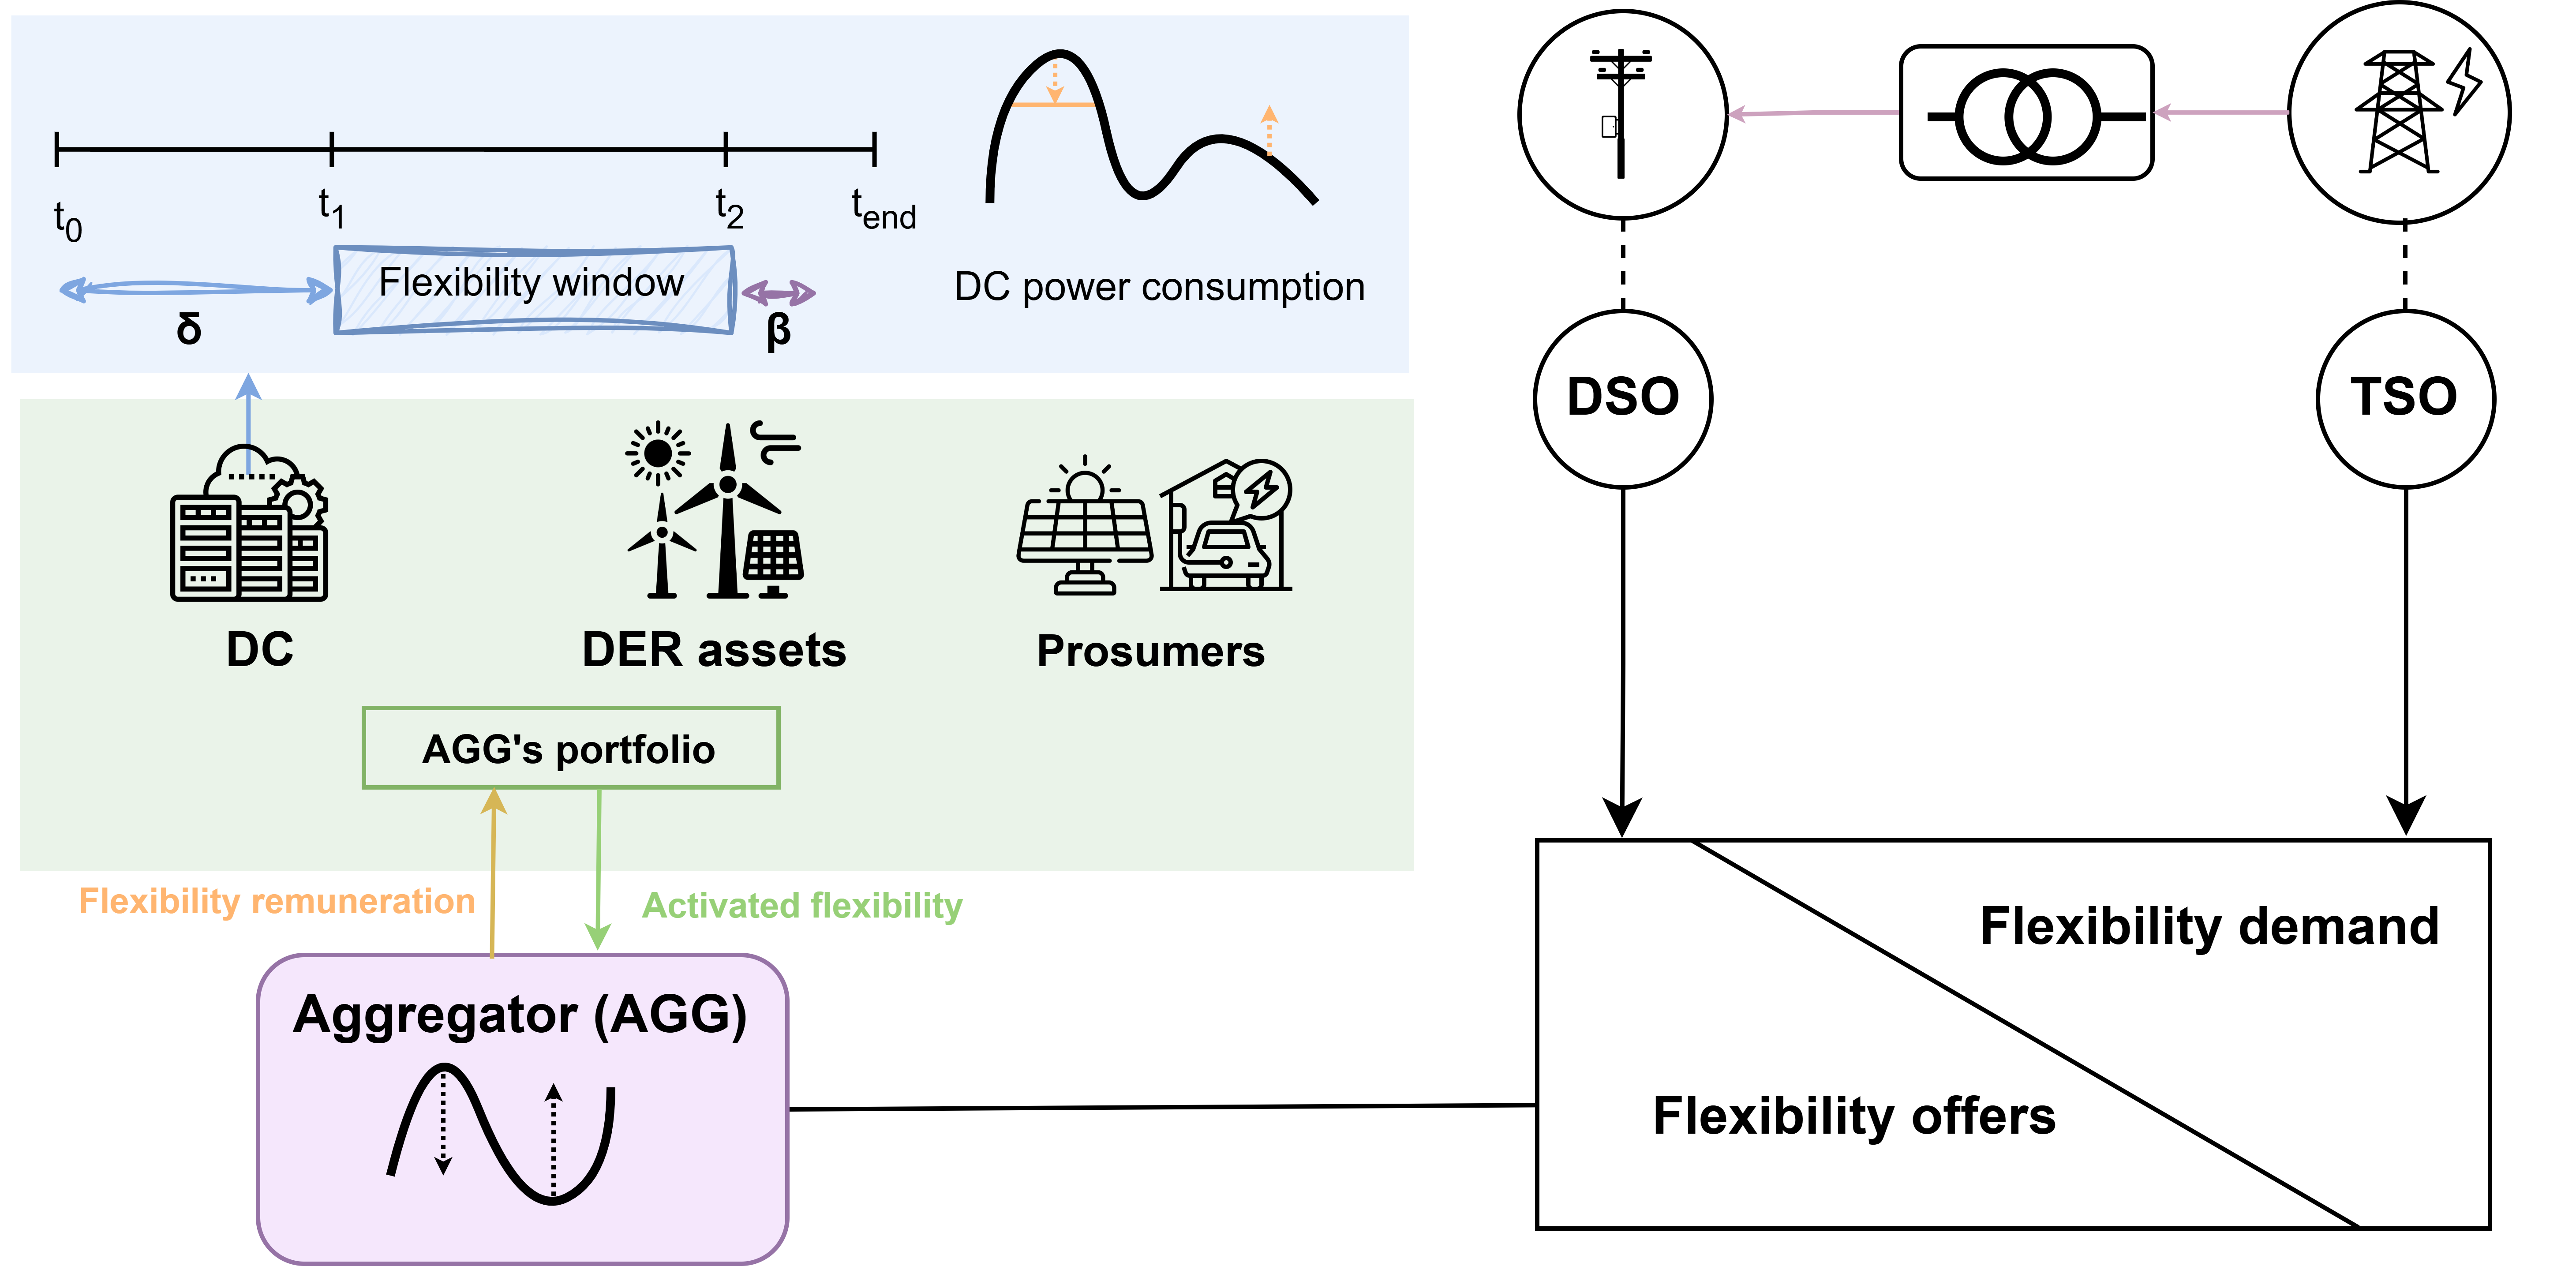
\includegraphics[width=14cm]{methodology_diagram.png  }
    \caption[Latency overview]{Illustration of the interaction between aggregator and DC derived from \cite{DEttorre2022}}
    \label{fig:AGG_ecosystem}
\end{figure}
These considerations give rise to the following three key problem statements, which will be further explored in Section \ref{results}

\begin{itemize}
    \item \textbf{A posteriori flexibility assessment}: What is the maximum theoretical flexibility that the DC could offer, assuming perfect foresight and ideal scheduling conditions? This establishes an upper bound for the flexibility potential across the workload.
    
    \item \textbf{LAD-Flex strategy}: How can the DC realistically offer flexibility to an aggregator, considering task durations, scheduling constraints, and the requirement that deferred tasks must fit within predefined flexibility offer windows?
    
    \item \textbf{Notification period optimization}: Given the constraints of the LAD-Flex strategy, what is the optimal notification time $\delta$ that maximizes the value of the flexibility provided, balancing the responsiveness of the DC with the preferences of the aggregator?
\end{itemize}
\section{Methodology}\label{methodology}
%Methodology section introduction
To ensure the reproducibility of this work, this section outlines the steps carried out to assess and optimize the flexibility potential of the studied DC. Fig. \ref{fig:methodology_diag} provides an overview of the interactions among the key entities in this study, along with their corresponding subsections within the manuscript. In Section \ref{a_posteriori}, the power model of the DC is developed, presenting the hypothesis to assess the consumed power, tied to the latency of each submitted task. This allows to determine the amount of power consumed, classified by the amount of latency. Focusing on the development of a possible strategy to be implemented, Section \ref{LAD-Flex_section} presents the LAD-Flex algorithm. Finally, the flexibility obtained by deferring tasks is complemented with the price the aggregator is willing to pay, in the form of a flexibility value function. This is outlined in Section \ref{notification_period_opt_section_methodology}, where the trade-off between the value of real-time flexibility and the amount of flexibility available is defined, to find the notification period that maximizes value for both actors.

\begin{figure}[!h]
    \centering
    \includegraphics[width=14.5cm]{methodology.drawionew.png}
    \caption[Latency overview]{Overview of the key components of the service for flexibility potential assessment using non-critical workloads}
    \label{fig:methodology_diag}
\end{figure}

\subsection{"A posteriori" flexibility assessment} \label{a_posteriori}
%Data decription
Prior to the flexibility assessment, the raw trace data undergoes pre-processing. To facilitate the reproducibility of the study, the main pre-processing steps are outlined as follows. The dataset contains detailed records of job submissions, task executions, and instance-level resource allocations. It is structured across multiple relational tables, including job-level metadata, task-level scheduling information and per-instance execution records. The resulting DataFrame included 7 columns, \texttt{task\_name}, \texttt{t\_request}, \texttt{start\_time}, \texttt{end\_time}, \texttt{plan\_GPU}, \texttt{duration}, \texttt{wait\_time} and \texttt{GPU\_type}. If \texttt{plan\_GPU} is less than 1, it indicates that the task uses a fractional portion of a GPU and supports gang scheduling; the value represents the percentage of a GPU allocated. Values greater than 1 indicate that the task requires one or more full GPUs. This information identifies the GPU model/group associated with a task, but it does not provide a reliable time-resolved mapping from each task to a specific physical GPU device and its measured utilization trace.

\begin{table}[h!]
\centering
\begin{tabular}{ll}
\toprule
\textbf{Column Name} & \textbf{Description} \\
\midrule
\texttt{task\_name}   & Identifier of the task \\
\texttt{t\_request}   & Timestamp when the task was requested \\
\texttt{start\_time}  & Timestamp when the task started execution \\
\texttt{end\_time}    & Timestamp when the task finished execution \\
\texttt{plan\_GPU}    & Number of GPUs allocated for the task \\
\texttt{duration}     & Total execution time of the task (in seconds) \\
\texttt{wait\_time}   & Latency of the task before execution (in seconds)  \\
\texttt{GPU\_type}    & Model of GPU(s) on which the instance(s) are executed \\
\bottomrule
\end{tabular}
\caption{Description of the columns in the task scheduling DataFrame.}
\label{tab:df_columns}
\end{table}

%Data cleaning and outliers removal
In a real operational setting, not all tasks can be executed successfully due to various reasons.  Tasks labeled as "failed", "running", or "waiting" are removed, as they do not represent completed workload behavior. Additionally, all entries with missing values for GPU, CPU, or memory usage are excluded from the analysis. 


\
%Formula to get power from GPU utilization (sum over different GPUs of heterogeneous cluster)
To evaluate the flexibility potential of the DC, an estimate of GPU-side IT power is required. However, the Alibaba trace does not provide measured per-device power telemetry, nor a reliable mapping from each task to a specific physical GPU utilization trajectory over time. The available information identifies the GPU type associated with a task together with the allocated GPU fraction, but not the instantaneous machine-level operating point of the underlying device. For this reason, this study adopts a first-order GPU power model in which power is approximated as proportional to the allocated utilization fraction for the corresponding GPU model/group. This model is used to construct workload-level estimates suitable for flexibility-potential assessment, rather than hardware-accurate GPU power characterization. The present framework therefore quantifies IT-side flexible power rather than precise facility demand, and it does not model the response of cooling, UPS, or auxiliary systems during flexibility activation.

Under this approximation, the utilization attributed to a task is treated as constant during its execution and equal to the GPU resources allocated by the scheduler. This enables consistent aggregation across heterogeneous GPU models/groups using the information available in the trace, while acknowledging that real GPU power curves are device-dependent and generally non-linear.

Under these assumptions, the instantaneous power consumption of the DC at time $t$ can be computed using Eq. ~\ref{eq:power_DC1}:

\begin{equation} \label{eq:power_DC1}
P^{DC}_{t} = \sum_{i=1}^{N} P^{node}_{it} = \sum_{i=1}^{N} \sum_{j=1}^{G_i} P^{GPU, nom}_{ij} \chi_{ijt}
\end{equation}

Here, $N$ denotes the number of node types, each containing different GPU models/groups, $G_i$ the number of GPUs in node type $i$, $P^{GPU, nom}_{ij}$ the nominal power assigned to GPU $j$ in node $i$, and $\chi_{ijt}$ the utilization estimate attributed to that GPU at time $t$ under the adopted approximation. 

In the case where all GPUs within a node type are considered homogeneous in terms of power characteristics and utilization, a simplified model can be used for efficiency. The total power consumption then reduces to:

\begin{equation} \label{eq:power_DC2}
P^{DC}_t = \sum_{i=1}^{N} G_i \cdot P^{GPU, nom}_i \cdot \bar{\chi}_{it}
\end{equation}

In this expression, $P^{GPU, nom}_i$ refers to the nominal power assigned to a single GPU in node type $i$, and $\bar{\chi}_{it}$ denotes the average allocated-utilization estimate of the tasks active on that GPU in node type $i$ at time $t$.

%Latency groups: non critical tasks identified if they had to wait more than X minutes
To assess the flexibility potential of the DC workload, tasks are grouped according to their observed queuing latency, defined as the time each task waited between submission and execution. Let $\mathcal{T}$ denote the set of all tasks. For each task $k \in \mathcal{T}$, the queuing latency $\lambda_k$ is computed as:

\begin{equation}
\lambda_k = \texttt{start\_time}_k - \texttt{t\_request}_k = \texttt{wait\_time}_k
\end{equation}

The task set $\mathcal{T}$ is partitioned into latency classes based on a series of non-overlapping intervals. Let $\mathcal{I} = \{ (a_1, b_1], (a_2, b_2], \dots, (a_L, b_L] \}$ denote a collection of latency intervals such that $a_{i+1} > b_i$ for all $i$, and optionally define a final group for tasks with latency exceeding the maximum bound. For each interval $(a_\ell, b_\ell] \in \mathcal{I}$, the corresponding latency class is defined as:

\begin{equation}
\mathcal{T}_{(a_\ell, b_\ell]} = \left\{ k \in \mathcal{T} \,\middle|\, a_\ell < \lambda_k \leq b_\ell \right\}
\end{equation}

An additional group for high-latency tasks can be defined as:

\begin{equation}
\mathcal{T}_{>b_L} = \left\{ k \in \mathcal{T} \,\middle|\, \lambda_k > b_L \right\}
\end{equation}

These groups enable conditional analysis of estimated GPU-side power by applying the power estimation models in Equations~\ref{eq:power_DC1} and~\ref{eq:power_DC2} to filtered task sets. Specifically, for each group $\mathcal{T}_{(a_\ell, b_\ell]}$, the aggregated estimated power consumption can be computed, assessing its deferrability, identifying segments of workload with inherent temporal flexibility.

To quantify the estimated GPU-side power consumption attributable to specific latency groups over a given time interval, a discrete-time summation is applied. Let $[t_1, t_2]$ be the time interval of interest, divided into time steps of duration $\Delta t$. For each latency group $\mathcal{T}_{(a_\ell, b_\ell]}$, the total energy consumed by its associated tasks during $[t_1, t_2]$ is computed as:

\begin{equation}
E^{(a_\ell, b_\ell]}_{[t_1, t_2]} = \sum_{t = t_1}^{t_2} P^{DC}_{t, \mathcal{T}_{(a_\ell, b_\ell]}} \cdot \Delta t
\label{eq:energy_group}
\end{equation}

Here, $P^{DC}_{t, \mathcal{T}_{(a_\ell, b_\ell]}}$ denotes the estimated GPU-side power at time $t$ obtained by considering only tasks belonging to the latency group $\mathcal{T}_{(a_\ell, b_\ell]}$ that are active at time $t$. This can be expressed as:

\begin{equation}
P^{DC}_{t, \mathcal{T}_{(a_\ell, b_\ell]}} = \sum_{k \in \mathcal{A}_{t}^{(a_\ell, b_\ell]}} P^{GPU, nom}_k \cdot \chi_k
\label{eq:power_group}
\end{equation}

where $\mathcal{A}_{t}^{(a_\ell, b_\ell]} \subseteq \mathcal{T}_{(a_\ell, b_\ell]}$ is the set of tasks from group $\mathcal{T}_{(a_\ell, b_\ell]}$ that are actively executing at time $t$, $P^{GPU, nom}_k$ is the nominal power assigned according to the GPU node type associated with task $k$, and $\chi_k$ is its corresponding allocated utilization fraction. These expressions enable estimated energy analysis within specific latency classes, allowing for the identification of time intervals and workload segments with inherent flexibility that could potentially be deferred or shifted. 

Fig. \ref{fig:latency} illustrates the hierarchical relationship between jobs, tasks, and instances, and clarifies the rationale behind focusing on task–instance latency rather than job–task latency. IT-workloads related power consumption primarily occurs during the execution of instances on GPUs, making task–instance granularity the most relevant level for energy-aware scheduling and flexibility analysis. Moreover, as detailed in Section \ref{case study}, the dataset reveals that only a small fraction of jobs contain multiple tasks. Therefore, treating each task independently introduces a negligible approximation, and this simplification is justified for the scope of this study. Furthermore, it is shown graphically how the duration of each task is determined by the difference of the time step between the end of the execution of the last instance and the start time of the first instance. 


% \begin{figure}[!h]
%     \centering
%     \includegraphics[width=14cm]{latency definition.png}
%     \caption[Latency overview]{Graphical Definition of Latency}
%     \label{fig:latency}
% \end{figure}

\begin{figure}[!h]
    \centering
    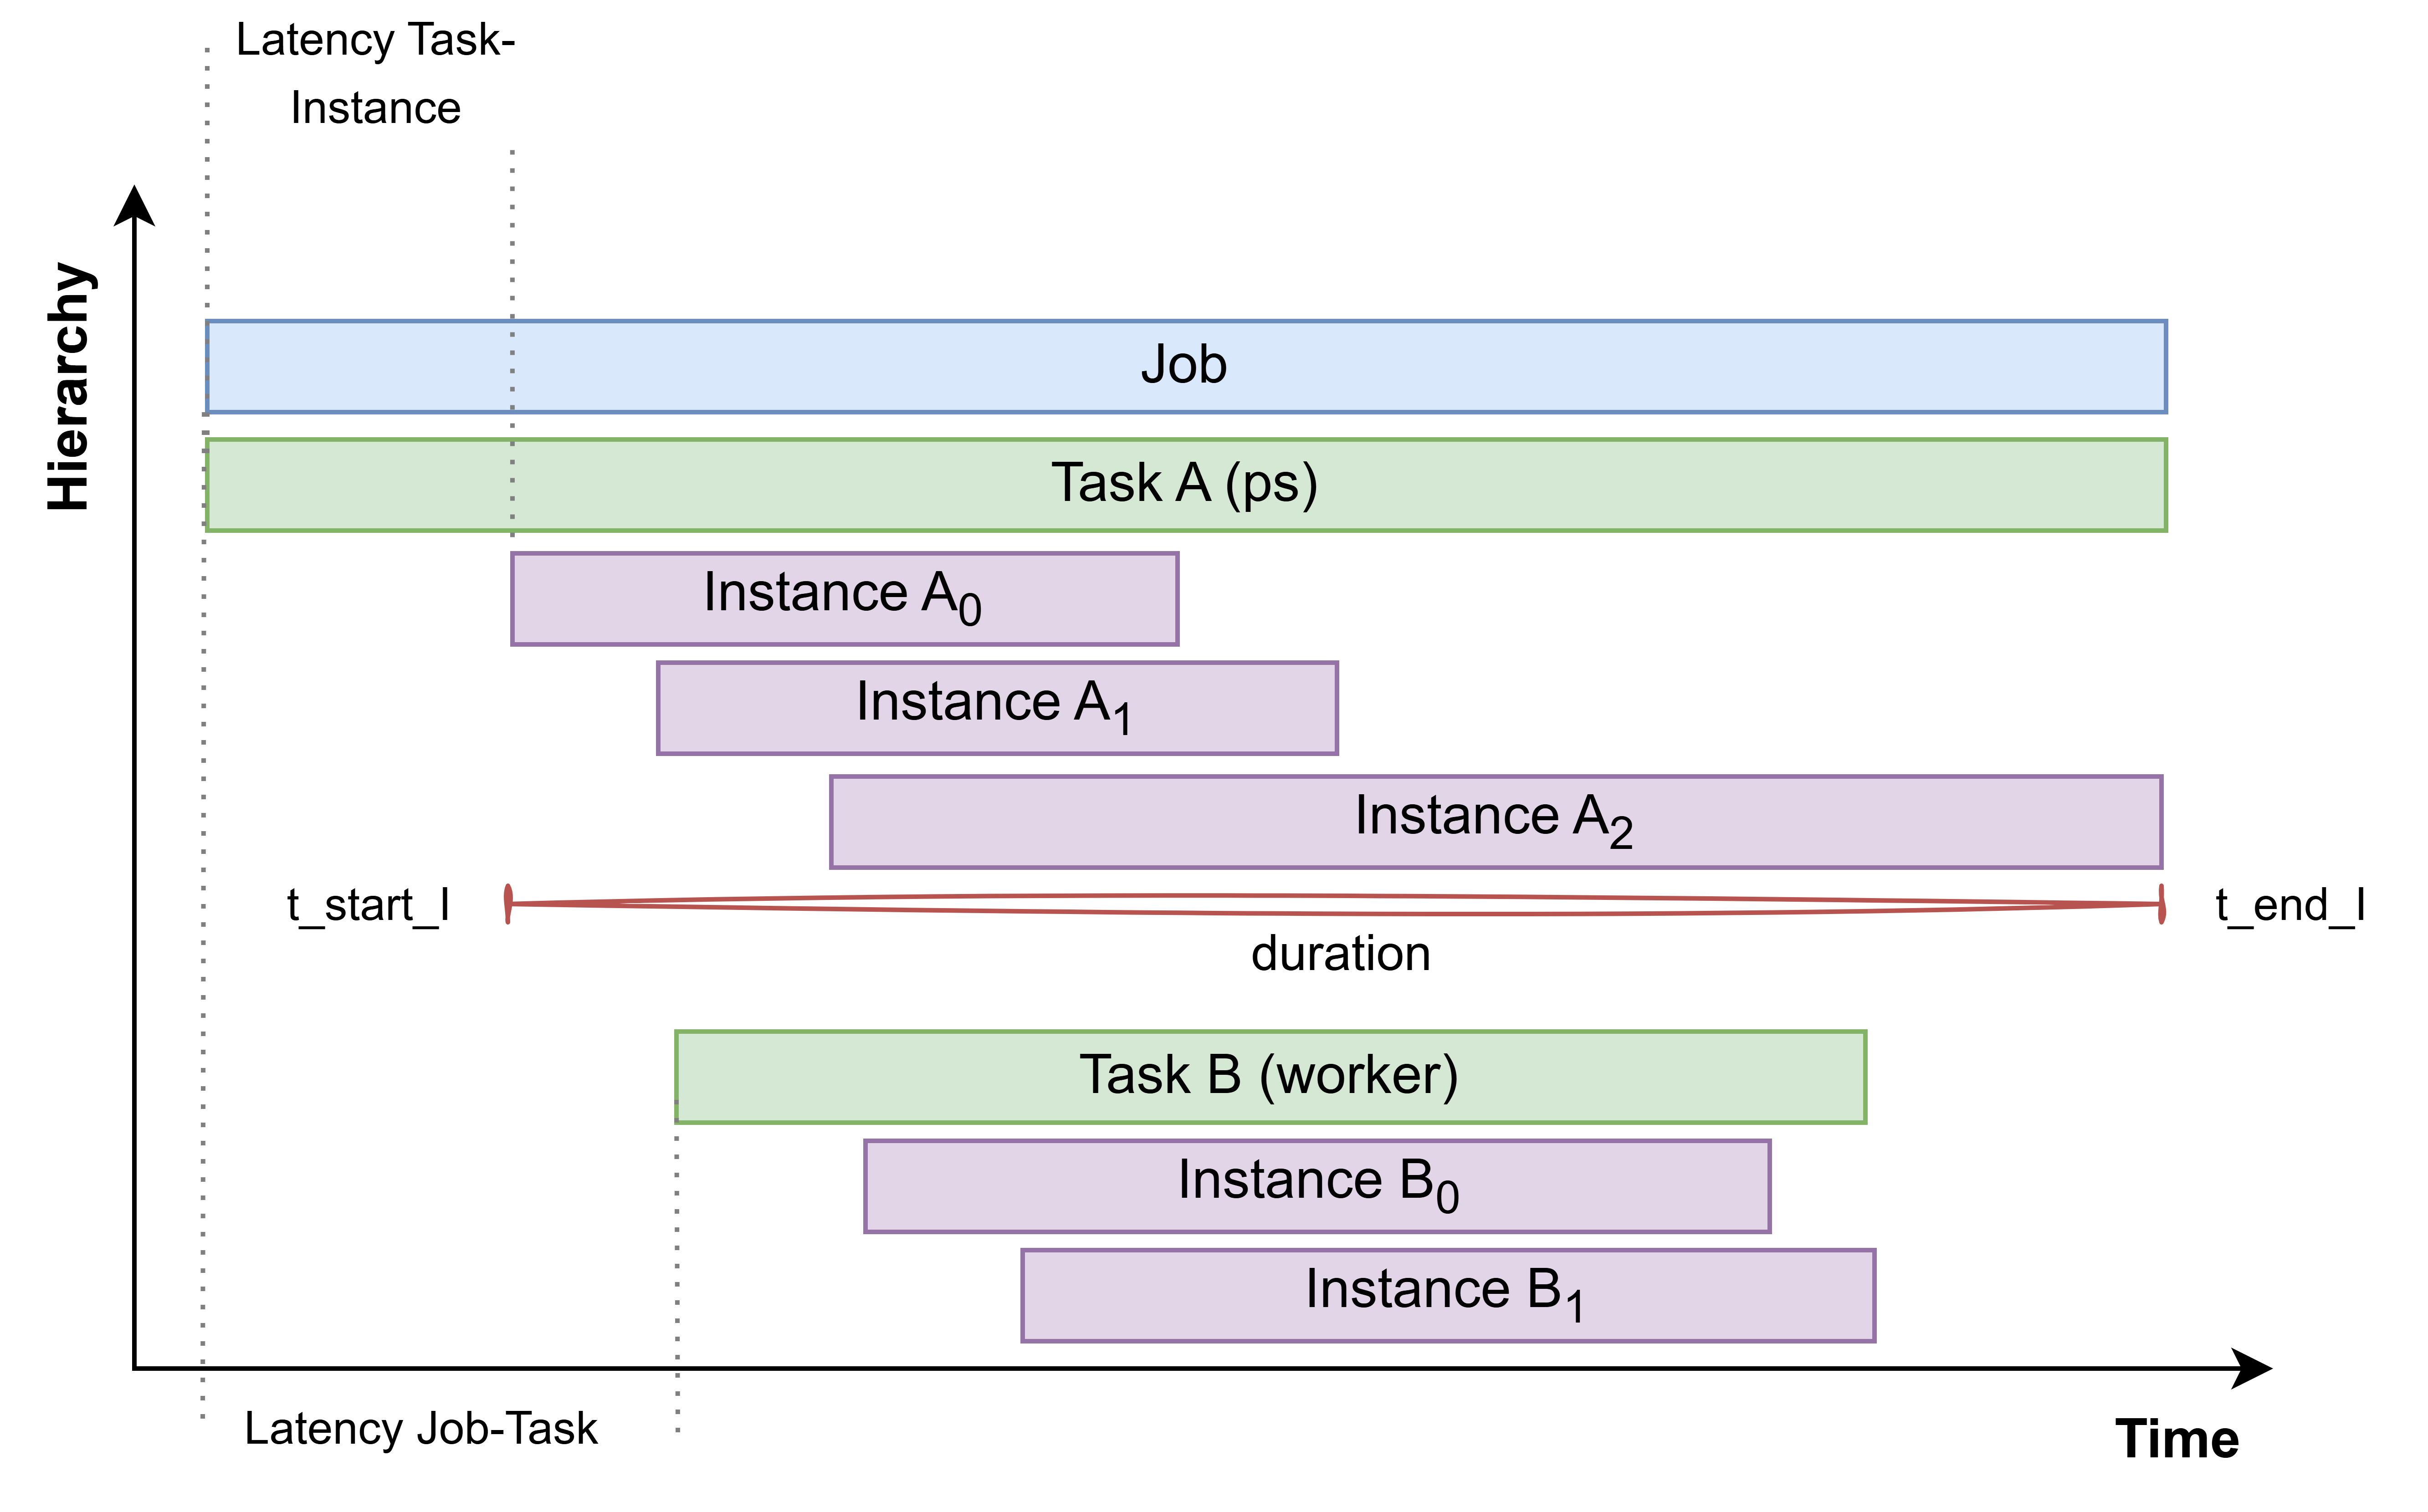
\includegraphics[width=14cm]{latencydiagram.png}
    \caption[Latency overview]{Illustration of job–task–instance hierarchy and latency definitions. The job shown consists of two tasks: a parameter server (Task A) and a worker (Task B). Although Task A is launched immediately upon job submission, its actual execution is delayed until Instance $A_0$ starts on a GPU. Then, after the initial job–task latency, Task B is launched and begins executing via its own instances. This decomposition illustrates why this study focuses on task–instance latency, where actual GPU activity, and thus power consumption, takes place.}
    \label{fig:latency}
\end{figure}

\subsection{LAD-Flex} \label{LAD-Flex_section}
Let us consider now the flexibility offered by the aggregator. This section models the bid requirements the DC must comply with, and the scheduling adjustments it needs to make to provide downward DR in the form of load shedding via deferral of non-critical tasks.

\subsubsection{Aggregator Flexibility Window}

The flexibility request is initiated by an external aggregator or determined by market requirements. This determines the notification to the DC of request of temporary reduction in power consumption. This request is defined by three key parameters: a notification time, the start of the flexibility window, and the duration of the reduction period.

Let \( t_0 \) be the time at which the DC is notified of an upcoming flexibility request. The actual flexibility window begins at time \( t_1 \), defined as:

\begin{equation}
    t_1 = t_0 + \delta
\end{equation}


where \( \delta \) is the notification lead time. The duration of the flexibility window is determined proportionally as:

\begin{equation}
    t_2 = t_1 + \eta \cdot \Delta T = t_0 + \delta + \eta \cdot \Delta T
\end{equation}

Here, \( \Delta T \) is a baseline duration unit (e.g., 1 hour), and \( \eta \) is a tunable scaling parameter used to explore the sensitivity of the strategy to longer or shorter flexibility windows. The full flexibility activation period is therefore:

\begin{equation}
    \text{Flexibility Window} = [t_1,\ t_2] = [t_0 + \delta,\ t_0 + \delta + \eta \cdot \Delta T]
\end{equation}

For this study, minimum capacity requirements are not imposed. This assumption is intentional: the objective of this study is not to demonstrate operational compliance with grid balancing requirements, but rather to quantify the latent flexibility potential under realistic scheduling and operational constraints. Indeed, the experimental scope is limited to approximately 6800 GPUs, representing a significant but scalable fraction of the DC. 

\subsubsection{Latency threshold}

A threshold latency value $\hat{\lambda}$ is defined to separate tasks into two categories: those that are time-sensitive ($\lambda_k \leq \hat{\lambda}$) and those that are potentially flexible ($\lambda_k > \hat{\lambda}$). The set of tasks identified as candidates for flexibility analysis is therefore defined as:

\begin{equation}
\mathcal{T}_{>b_L} = \left\{ k \in \mathcal{T} \,\middle|\, \lambda_k > \hat{\lambda} \right\}
\end{equation}

This classification enables focused analysis on workloads that are not immediately critical, assuming they are suitable to be studied for the assessment of flexibility potentials of the DC. It should be noted that this classification operates at the individual task level and does not account for potential inter-task dependencies within multi-task jobs. However, as shown in Section~\ref{case study}, multi-task jobs represent only 2.5\% of the cleaned dataset, and deferred tasks are not cancelled but postponed, limiting the scope of possible cascading effects on downstream tasks.

\subsubsection{Incorporating task duration prediction uncertainty} \label{prediction_uncertainty_methods}
As the aim of this work is to match deferrable tasks with a specific flexibility window, knowing the expected duration of each task is essential. Tasks are assumed to run to completion without interruption and are not split over multiple time periods. 
The previous section \ref{a_posteriori} presented a flexibility assessment based on grouping tasks by observed latency without considering their execution profile. While this approach enabled estimation of the theoretical load shifting potential, it did not account for operational constraints that influence feasibility under real-time conditions.

Although the DC under study is agnostic to task progress and other metadata required to directly determine task durations, it is reasonable to assume that duration estimates can be made available. This assumption is supported by the growing integration of predictive analytics in modern DC scheduling systems, including deep-learning workload characterization and prediction \cite{Hu2021}, interference-aware GPU utilization forecasting \cite{Yeung2022}, machine-learning-based GPU execution time prediction \cite{Amaris2016}, and uncertainty-scaled task completion time estimation \cite{Kawaguchi2024}. Additionally, the publishers of the dataset report that task durations can be predicted with a %percentage 
Mean Absolute Error (MAE) below 25\% for 78\% of tasks recurring at least five times in the trace \cite{Weng2022}. These findings indicate that, even in systems without explicit predictive modules, duration forecasting is a feasible assumption, particularly for facilities running a significant proportion of recurring jobs.

The forecasting model from \cite{Weng2022}, however, is not publicly available. To approximate this behavior and evaluate the robustness of the proposed flexibility strategy under realistic conditions, a simulated prediction uncertainty is directly introduced into our model. This approach enables to analyze how imperfect duration knowledge affects deferral decisions, without relying on a specific prediction algorithm.

\paragraph{Stochastic modeling of predicted durations}

Let $d_k$ denote the true (observed) duration of task $k$ from the historical trace. To simulate predicted durations available at scheduling time, it is defined:

\begin{equation}
    \hat{d}_k = d_k + \epsilon_k, \quad \text{where } \epsilon_k \sim \mathcal{N}(0, \sigma_k^2)
\end{equation}

where $\epsilon_k$ is a normally distributed zero-mean error term, and $\sigma_k$ represents the standard deviation of the prediction error. It is assumed the prediction error scales with task length:

\begin{equation}
    \sigma_k = \zeta \cdot d_k
\end{equation}

This formulation reflects two key characteristics observed in production DC scheduling systems \cite{Hu2021, Yeung2022}: prediction errors tend to be proportional to task duration rather than constant, and errors are approximately symmetrically distributed around the true value. The zero-mean assumption ensures that the model does not systematically overestimate or underestimate durations, which would introduce bias in the flexibility assessment. 

\paragraph{Exclusion of long tasks}
Tasks with durations that significantly exceed the flexibility window, such as those that last several hours or more, are excluded from the deferrability assessment. Although deferring such tasks may technically provide load-shedding potential, the resulting rebound effect, i.e., shifting large power consumption to non-flexible periods-makes them less desirable from a flexibility activation perspective. In practice, these tasks are typically scheduled with substantial advance planning and are less amenable to short-notice rescheduling or deferral.

By filtering these out, the strategy prioritizes short and medium-length tasks that can be more precisely aligned with the flexibility window and rescheduled without destabilizing other operational periods.


\subsubsection{Flexibility window parameters: overhang and buffer period}


In order to account for misalignments in task timing with the flexibility window, two internal parameters are introduced: a buffer period $\gamma_{\text{buffer}}$ and an overhang tolerance coefficient $\beta$.

These parameters are not dictated by the aggregator but rather reflect internal scheduling choices made by the DC to defer as many reasonable tasks as possible, while managing rebound effects within acceptable limits. %For example, a very long-running task should not be deferred, while a task that finishes just after the end of the flexibility window should be deferred.
For example, a long-running task should not be deferred, whereas a task that completes shortly after the end of the flexibility window is a suitable candidate for deferral.
To avoid excluding tasks that finish marginally after the flexibility window but are otherwise suitable for deferral, the window is extended slightly beyond $t_2$:

\begin{equation}
    t_{\text{end}}^{\text{flex}} = t_2 + \gamma_{\text{buffer}}
\end{equation}

Here, $\gamma_{\text{buffer}}$ is a configurable parameter for DC operators (e.g., 30–60 minutes), representing the allowable extension beyond $t_2 $, i.e.,  the official end of the flexibility window, for task completion. This enables greater flexibility activation, with only minor rebounds external to the window.

Furthermore, to avoid strictly requiring all task execution to fit within $[t_1, t_2]$, an overhang threshold is defined $\beta \in [0, 1]$, which determines how much of the task's duration may lie outside the flexibility window without disqualifying it from deferral. Let $\hat{d}_i$ denote the predicted duration of task $i$, and $t_i^{\text{start}}$ and $t_i^{\text{end}}$ its planned start and end times. The task is accepted if the overhang before and after the flexibility window does not exceed a fraction $\beta$ of the task's duration:

\begin{equation}
    t_1 - t_i^{\text{start}} \leq \beta \cdot \hat{d}_i \quad \text{and} \quad t_i^{\text{end}} - t_2 \leq \beta \cdot \hat{d}_i
\end{equation}

Putting these considerations together, a task $i$ is considered deferrable under the LAD-Flex strategy if:

%OBS: removed subequations as it reset the equations counter
% \begin{subequations}
\label{eq:deferrable_conditions}
\begin{numcases}{\text{Deferrable}_i \iff}
    t_i^{\text{start}} \geq t_0 \quad & \text{(Start after notification)} \label{case:start} \\
    t_i^{\text{end}} \leq t_2 + \gamma_{\text{buffer}} \quad & \text{(End before buffer)} \label{case:end} \\
    t_1 - t_i^{\text{start}} \leq \beta \hat{d}_i \quad & \text{(Start overhang)} \label{case:start_overhang} \\
    t_i^{\text{end}} - t_2 \leq \beta \hat{d}_i \quad & \text{(End overhang)} \label{case:end_overhang}
\end{numcases}
% \end{subequations} 


These conditions are visually represented in Fig. \ref{fig:flex_conditions}.

\begin{figure}[!h]
    \centering
    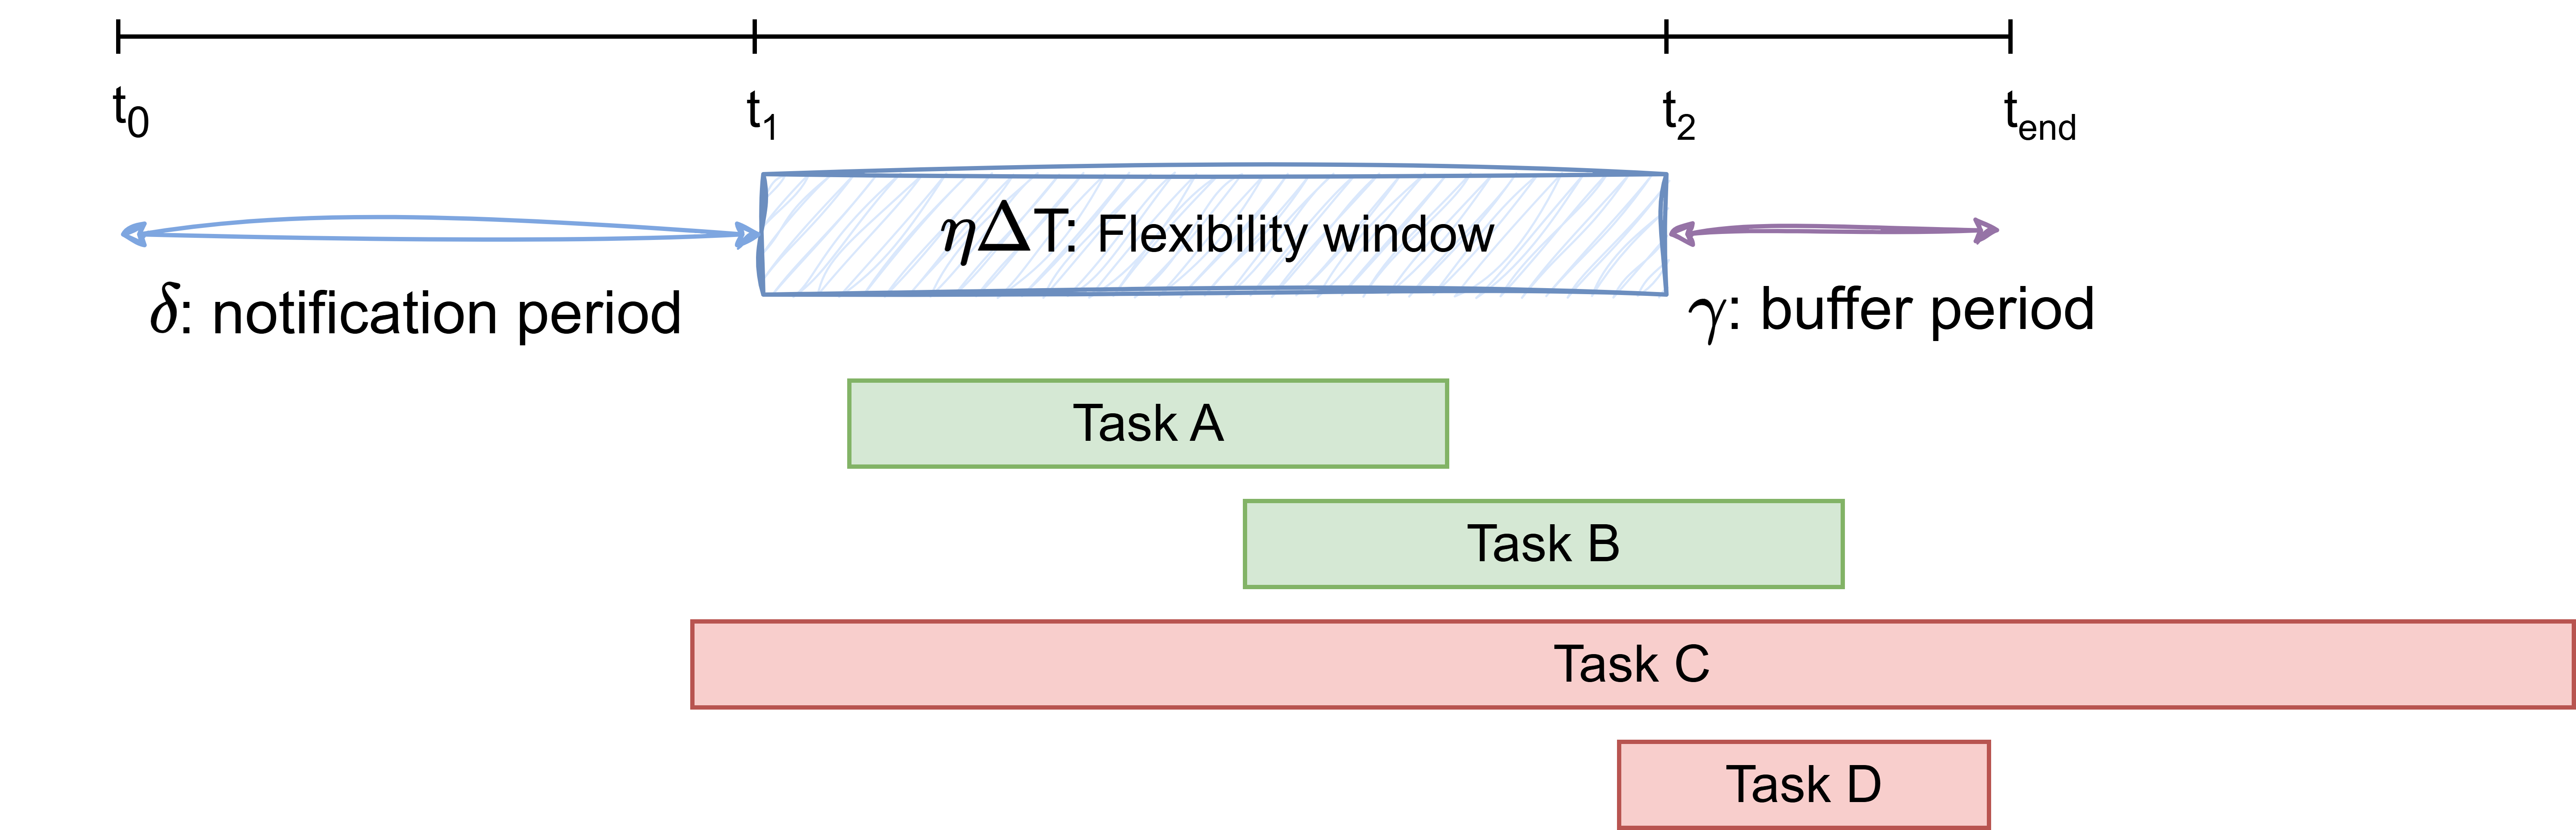
\includegraphics[width=14cm]{task_flex_conditions.png}
    \caption[Latency overview]{Examples of deferred (green) and non-deferred (red) tasks with respect to the flexibility window and overhang constraints. Task A and Task B satisfy all the conditions, where as Task C does not comply with condition~\ref{case:end}, as it finishes after the admitted overhang period. Assuming in this case $\beta_{overhang}=0.5$, task D does not comply with condition~\ref{case:end_overhang} and is thus not accepted for deferral}
    \label{fig:flex_conditions}
\end{figure}


\subsection{Notification period optimization}\label{notification_period_opt_section_methodology}
Once the set of deferrable tasks has been identified through the LAD-Flex strategy, the interaction between the aggregator and DC can be further improved. In particular, an optimization framework is introduced to determine the optimal notification period length that a DC should adopt to maximize the returns from flexibility activation.

The aggregator is assumed to be an independent entity participating in wholesale electricity markets. It can issue flexibility requests to the DC with varying levels of advance notice, to meet market needs more effectively.

From a system design perspective, a key trade-off arises:
\begin{itemize}
    \item A longer notification period (\( \delta \)) allows the DC to schedule a greater number of tasks flexibly, increasing the total deferrable energy.
    \item A shorter notification period enhances the real-time value of the flexibility, since near-instantaneous response commands higher compensation in flexibility markets \cite{Villar2018} and real-time demand response programs \cite{Conejo2010, MohsenianRad2010}.
\end{itemize}

To capture this trade-off, the unit value of flexibility \( V(\delta) \) is modeled as a decreasing function of \( \delta \): as the notification period increases, the flexibility becomes less valuable to the aggregator because it can no longer serve time-critical market products. Specifically, a smoothed decay function is adopted:

\begin{equation}
V(\delta) = V_{\min} + \frac{V_{\max} - V_{\min}}{1 + \left( \frac{\delta}{\tau} \right)^{\alpha}}
\label{smooth_decay}
\end{equation}

where \( V_{\min} \) and \( V_{\max} \) represent the lower and upper bounds of the value (€/kWh), \( \tau \) determines the characteristic time scale of value decay, and \( \alpha \) controls the steepness of the decline. In this formulation, \( V_{\min} \) and \( V_{\max} \) define empirically informed bounds on flexibility remuneration, while \( \tau \) and \( \alpha \) are shape parameters. They are not directly estimated from historical electricity market data but are instead varied as scenario parameters to represent alternative plausible aggregator valuation profiles, allowing the framework to assess the robustness of the optimal notification period under different assumptions on the time-sensitivity of flexibility remuneration.

This trade-off is formalized as a univariate optimization problem. Let \( V(\delta) \) denote the unit value of flexibility and \( F(\delta) \) the quantity of deferrable energy available under LAD-Flex at a given notification period \( \delta \). The total financial return \( R(\delta) \) is expressed as:
\begin{equation} \label{eq:max_returns}
    R(\delta) = V(\delta) \cdot F(\delta)
\end{equation}

The objective is to identify the optimal notification period \( \delta^* \) that maximizes the return function:
\begin{equation}
    \delta^* = \underset{\delta}{\arg\max} \; R(\delta)
\end{equation}

The resulting value of \( \delta^* \) represents a point that optimizes the aggregator’s valuation of the flexibility and the DC’s ability to deliver it. By solving this problem, both entities converge on a notification strategy that aligns economic incentives with technical feasibility.


\section{Case Study}\label{case study}
\subsection{Case study assumptions}
To assess the flexibility potential of the DC, this section outlines the key assumptions adopted in the case study. First, it is assumed that once a task begins execution, it runs to completion without interruption; task fragmentation across multiple time periods is not considered in this analysis. Given that GPUs are significantly more energy-intensive than CPUs and that a larger share of IT workload-related power is allocated to GPUs, particularly for AI tasks \cite{LLM}, this study focuses on estimated GPU-side power. As the raw dataset does not include measured time-series power traces or machine-level monitoring that would permit calibration of device-specific nonlinear power curves, GPU power is estimated using the class-based model introduced in Section \ref{a_posteriori}.
The considered machine specifications are summarized in Table \ref{tab:specs}. The nominal power values are taken from commercial datasheets for the identified GPU models/groups; for the anonymized "Misc." category, a representative nominal value is assumed, and the "N/A" GPU entries are excluded from the estimated GPU-power analysis. CPUs and memory are not included in the present power calculation, as their contribution is assumed to be secondary relative to GPUs for the workloads under study. Accordingly, facility-level response and short-term PUE effects remain outside the modeled scope of the present analysis.

\begin{table}[h!]
\centering
\caption{System configurations in the PAI production cluster \cite{Weng2022}}
\label{tab:specs}
\begin{tabular}{lccccc}
\toprule
\textbf{\#CPUs} & \textbf{Mem (GiB)} & \textbf{\#GPUs} & \textbf{GPU type} & \textbf{\#Nodes} & \textbf{$P^{nom} (W)$} \\
\midrule
 64  & 512       & 2 & P100        & 798 &  250 \\
 96  & 512       & 2 & T4          & 497 & 70\\
 96  & 512       & 8 & Misc.       & 280 & 300\\
 96  & 384       & 8 & V100M32 & 135  & 300\\
 96  & 512/384   & 8 & V100    & 104 & 200\\
 96  & 512       & 0 & N/A         & 83 & N/A \\
\bottomrule
\end{tabular}
\end{table}


 
As part of the dataset anonymization process, all original date and time information was reset, even though the data was originally recorded between 2019 and 2020. As a result, the timestamps in the dataset default to the Unix epoch year of 1970. For consistency and reproducibility, this study refers to the sample week using the trace-provided dates, specifically from "01/02/1970" to "08/02/1970", even though these dates do not reflect the actual period of data collection.

Analysis of the cleaned dataset reveals that 97.5\% of jobs consist of a single task, with only 2.5\% containing multiple tasks. This confirms that workflow-level dependencies across tasks within the same job are structurally rare in the studied workload, and supports the assumption introduced in Section~\ref{a_posteriori} that treating tasks independently introduces a negligible approximation.

Further describing the data, Fig. \ref{fig:A_1a} shows the Cumulative Distribution Function (CDF) of task duration across the recorded trace. The distribution is heavily skewed, with a long tail indicating the presence of a small number of very long-running tasks, while the vast majority of tasks are relatively short. A more exhaustive characterization of this workload trace is presented in \cite{Weng2022}.

Fig. \ref{fig:B_1b}, on the other hand, presents a scatter plot of energy consumption as a function of task duration, where different GPU types are distinguished by color. The plot reveals distinct linear trends associated with different machine types, reflecting the varying power characteristics and computational efficiencies of each GPU class.

Anticipating that the flexibility windows considered for the Baseline scenario are at most 3~hours in length, the dataset is split into two categories:
\begin{itemize}
    \item \textit{Short-running tasks}: duration $<$ 3 hours
    \item \textit{Long-running tasks}: duration $\geq$ 3 hours
\end{itemize}

This threshold is visually highlighted in Fig. \ref{fig:B_1b}. This categorization supports the analysis of energy deferral strategies under realistic time-bound flexibility scenarios.

Table~\ref{tab:task_summary_duration} complements the visual analysis by quantifying the energy and wait time characteristics of the two task categories. While short tasks greatly outnumber long tasks, the total energy consumption is significantly higher for long tasks. This is expected, as longer tasks often correspond to more resource-intensive computations. Interestingly, average wait times are comparable between the two groups, though long tasks exhibit slightly higher standard deviation.

Given the limited time window (up to 4 hours for the Intraday scenario) assumed for real-time or near-term energy flexibility bidding, the deferrability strategies proposed in this work are limited to short-running tasks. These tasks are more compatible with the required response times and durations of flexibility signals. Long-running tasks may require different approaches such as day-ahead scheduling, reservation systems, or integration with longer-term flexibility programs, which will not be covered in this study.

\begin{figure}[!h]
    \centering

    \begin{subfigure}[b]{0.9\textwidth}
        \centering
        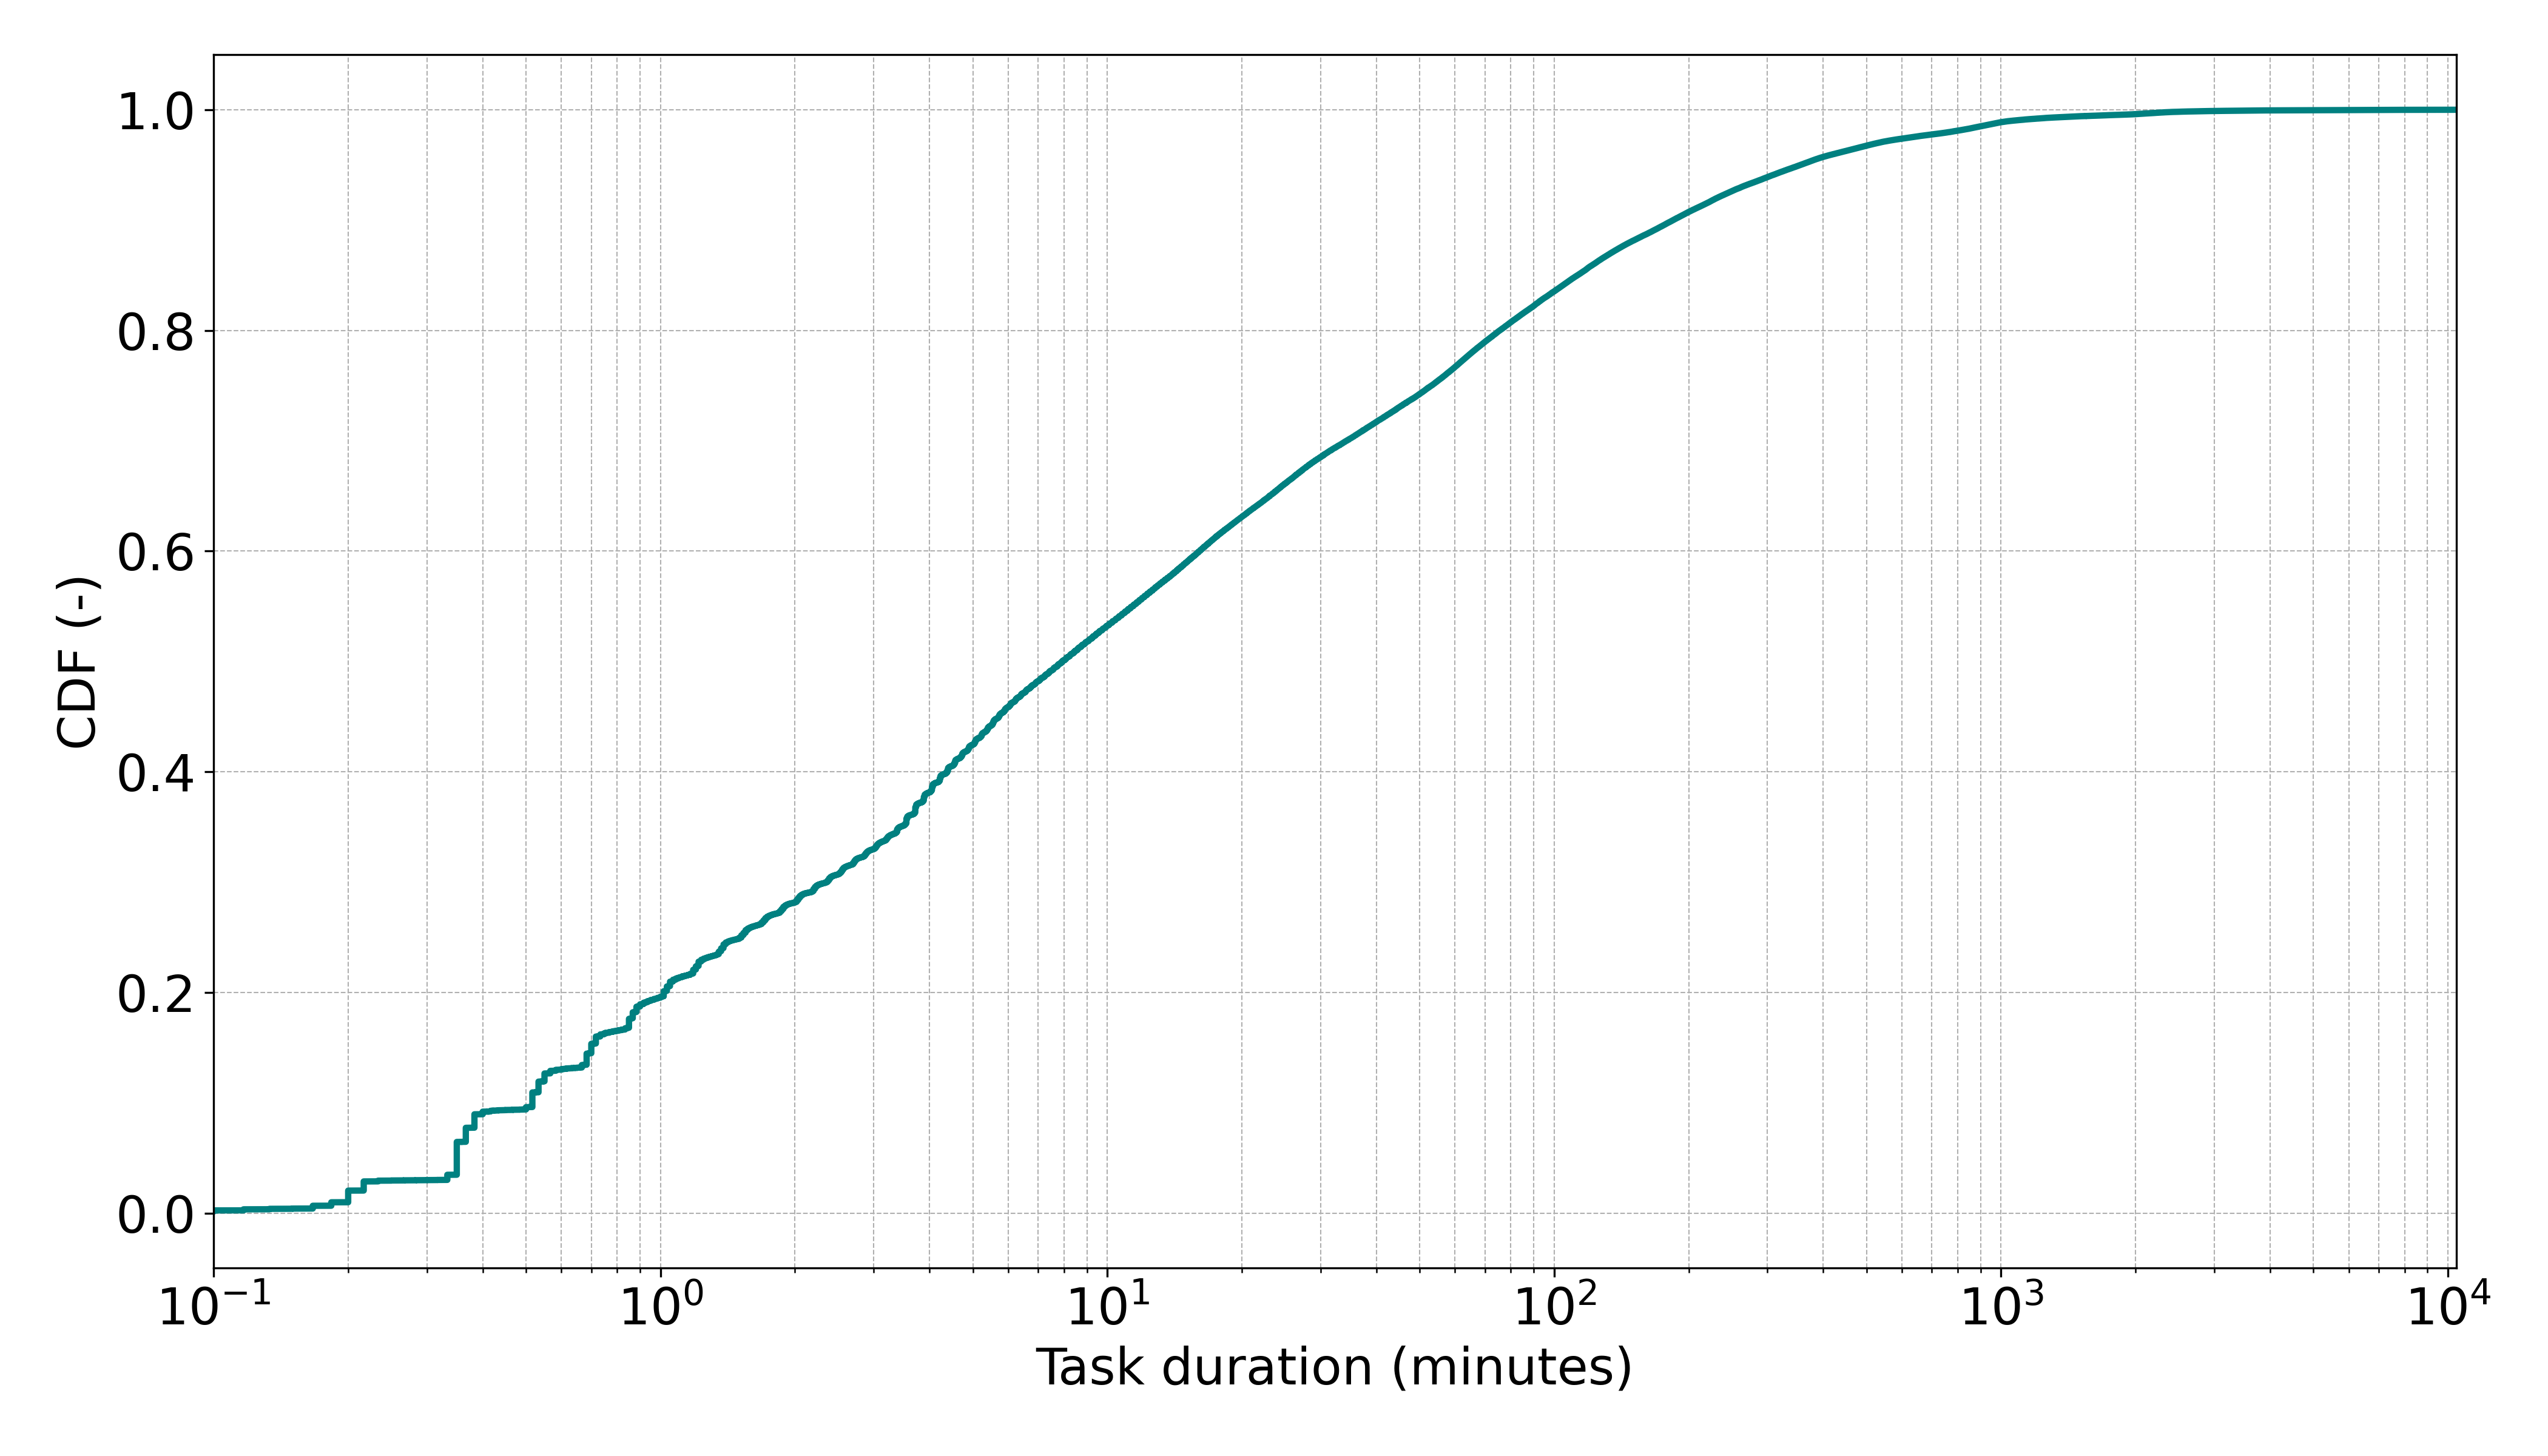
\includegraphics[width=\linewidth]{A.png}
        \caption{}
        \label{fig:A_1a}
    \end{subfigure}

    \vspace{0.5cm} % optional spacing between images

    \begin{subfigure}[b]{0.9\textwidth}
        \centering
        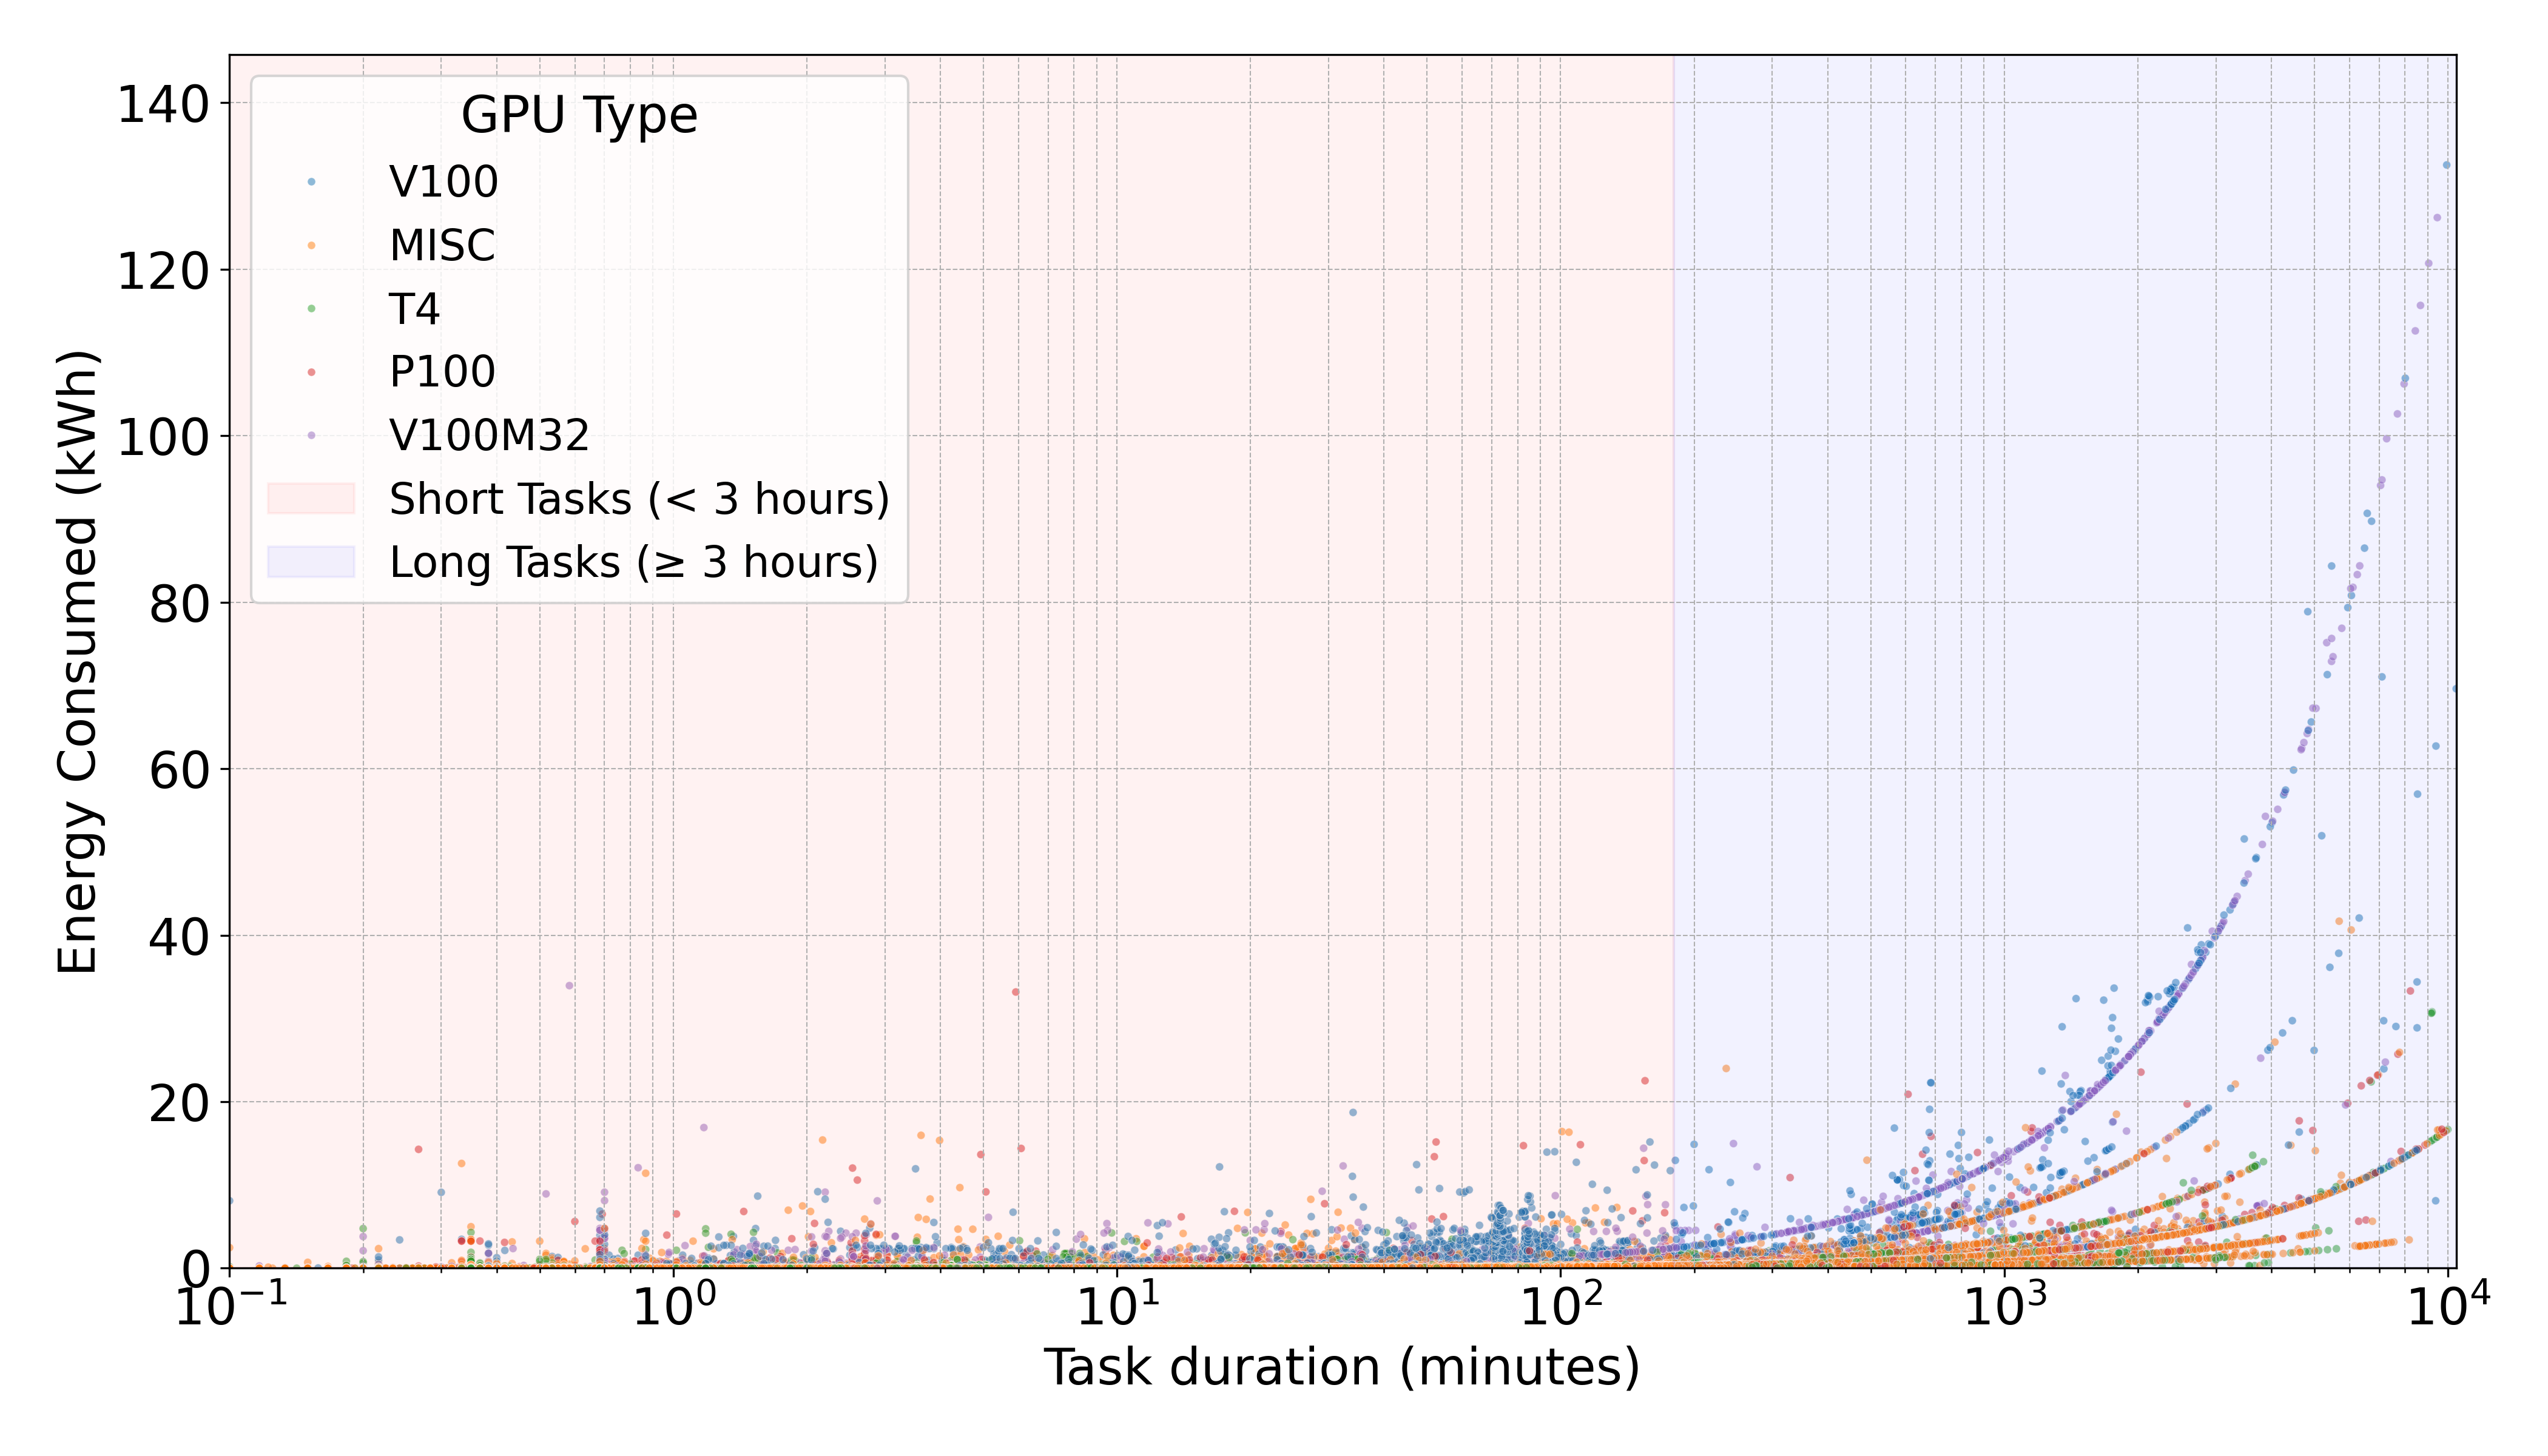
\includegraphics[width=\linewidth]{B.png}
        \caption{}
        \label{fig:B_1b}
    \end{subfigure}

    \caption[Latency overview]{Overview of task duration and energy consumption in the trace: 
(a) CDF of task durations, (b) Scatter plot of energy consumed versus task duration, colored by GPU type. A 3-hour threshold is used to distinguish short from long-running tasks.}
    \label{fig:cdf_duration}
\end{figure}

\begin{table}[h!]
\centering
\caption{Summary of task energy consumption and wait times divided by task duration}
\label{tab:task_summary_duration}
\begin{tabular}{lcc}
\toprule
\textbf{Metric} & \textbf{Long Tasks} & \textbf{Short Tasks} \\
\midrule
Total Energy Consumed (kWh)       & 68,327.60   & 24,721.92 \\
Number of Tasks                   & 74,991      & 657,699   \\
Average Wait Latency (seconds)       & 491.15      & 364.58    \\
Std Dev of Latency (seconds)    & 4,665.61    & 4,190.39  \\
\bottomrule
\end{tabular}
\end{table}

\subsection{Flexibility Scenarios and Market Context}\label{Case_study_scenarios}

To evaluate the LAD-Flex under realistic grid service requirements, three distinct flexibility scenarios are analyzed, each reflecting different market mechanisms prevalent in European electricity systems. The scenarios represent a spectrum of response timeframes and delivery requirements, enabling assessment of DC flexibility potential across different conditions. Table~\ref{tab:scenario_parameters} summarizes the parameter configurations for all three scenarios.

\begin{table}[htbp]
\centering
\caption{LAD-Flex parameter configurations across market scenarios}
\label{tab:scenario_parameters}
\begin{tabular}{lccc}
\toprule
\textbf{Parameter} & \textbf{Baseline} & \textbf{mFRR} & \textbf{Intraday} \\
\midrule
Latency threshold ($\hat{\lambda}$) & 10 min & 3 min & 30 min \\
Notification period ($\delta$) & 60 min & 15 min & 3 h \\
Flexibility window ($\eta\Delta T$) & 3 h & 1 h & 4 h \\
Overhang tolerance ($\beta$) & 0.7 & 0.9 & 0.8 \\
Buffer period ($\gamma_{\text{buffer}}$) & 60 min & 20 min & 120 min \\
\bottomrule
\end{tabular}
\end{table}

\subsubsection{Baseline Scenario}
The Baseline scenario models participation in general aggregator-coordinated flexibility programs, where load reductions commitments are made with moderate advance notice. This represents the foundational case analyzed throughout the paper and serves as the reference for evaluating alternative market configurations.

The latency threshold of $\hat{\lambda} = 10$ min balances responsiveness with a sufficiently large pool of flexible workloads. Tasks with queuing latency exceeding 10 minutes are candidates for deferral, ensuring that rescheduling does not impact time-sensitive operations. The notification period of $\delta = 60$ min provides adequate time for workload replanning without requiring day-ahead commitment, typical of aggregator-operated flexibility products that coordinate portfolios of distributed resources.

The flexibility window of $\eta\Delta T = 3$ h aligns with standard aggregator flexibility products that balance sustained load reduction with operational feasibility. An overhang tolerance of $\beta = 0.7$ permits up to 70\% of a task's duration to extend beyond the flexibility window boundaries, reducing over-conservative filtering while maintaining alignment with aggregator requirements. The buffer period of $\gamma_{\text{buffer}} = 60$ min accommodates minor scheduling imperfections, allowing tasks to complete up to 60 minutes after the official window end and reducing rebound concentration. This scenario serves as the reference case for establishing baseline flexibility potential before exploring alternative market participation pathways.

\subsubsection{Manual Frequency Restoration Reserves Scenario}

This scenario models participation in mFRR markets, which require rapid activation to address frequency deviations and power imbalances. European TSOs operating under ENTSO-E guidelines typically require mFRR resources to activate within 15 minutes and sustain delivery for 1-2 hours~\cite{ENTSOE_MARI_IG_v1_7}. The LAD-Flex parameters are adapted accordingly to meet these stringent operational requirements.

The latency threshold is reduced to $\hat{\lambda} = 3$ min, meaning more tasks will be marked as deferrable, increasing the flexibility volume with short notice time. The notification period of $\delta = 15$ min aligns with mFRR activation times specified in ENTSO-E balancing guidelines, representing near-real-time response capability.

The flexibility window is shortened to $\eta\Delta T = 1$ h to reflect typical mFRR activation durations. Although this limits the total energy that can be deferred, it matches grid operator expectations for balancing service delivery windows. To compensate for the shorter window and tighter latency constraint, the overhang tolerance is increased to $\beta = 0.9$, allowing tasks that nearly fit within the 1 h period to still qualify. The buffer period is reduced to $\gamma_{\text{buffer}} = 20$ min. This scenario targets DCs seeking to participate in high-value balancing markets where responsiveness commands premium compensation, despite potentially lower flexibility volumes compared to longer-notice products.

\subsubsection{Intraday Flexibility Market Scenario}

The intraday flexibility scenario reflects participation in continuously coupled intraday electricity markets across Europe. Under the Single Intraday Coupling (SIDC) framework, these markets facilitate continuous cross-zonal trading from day-ahead market closure until shortly before delivery. The intraday timeframe provides market participants with the opportunity to rebalance positions as updated information becomes available, including revised renewable generation forecasts, outages, and other operational developments \cite{ENTSOE_Market_Report_2024}.

The latency threshold is increased to $\hat{\lambda} = 30$ min, reflecting the longer planning horizon, ensuring that only less time sensitive tasks are chosen for deferral. This reduces the deferrable workload pool compared to the baseline and mFRR scenarios, but is compensated by longer notification periods and flexibility activation windows. Indeed, the notification period of $\delta = 3$ h positions the DC within the typical intraday trading window, where aggregators issue flexibility requests several hours before delivery to balance portfolios and optimize market positions.

The flexibility window is extended to $\eta\Delta T = 4$ h to align with standard intraday product durations. The extended window enables greater total energy deferral compared to mFRR's 1-hour activation while remaining within practical operational limits for workload management.

An overhang tolerance of $\beta = 0.8$ is chosen, and the buffer period is extended to $\gamma_{\text{buffer}} = 120$ min.

\subsection{Flexibility bid requirements}
As discussed in Section~\ref{notification_period_opt_section_methodology}, it is assumed that shorter notification periods are valued more highly by the aggregator than longer ones. 


\begin{figure}[!h]
    \centering
    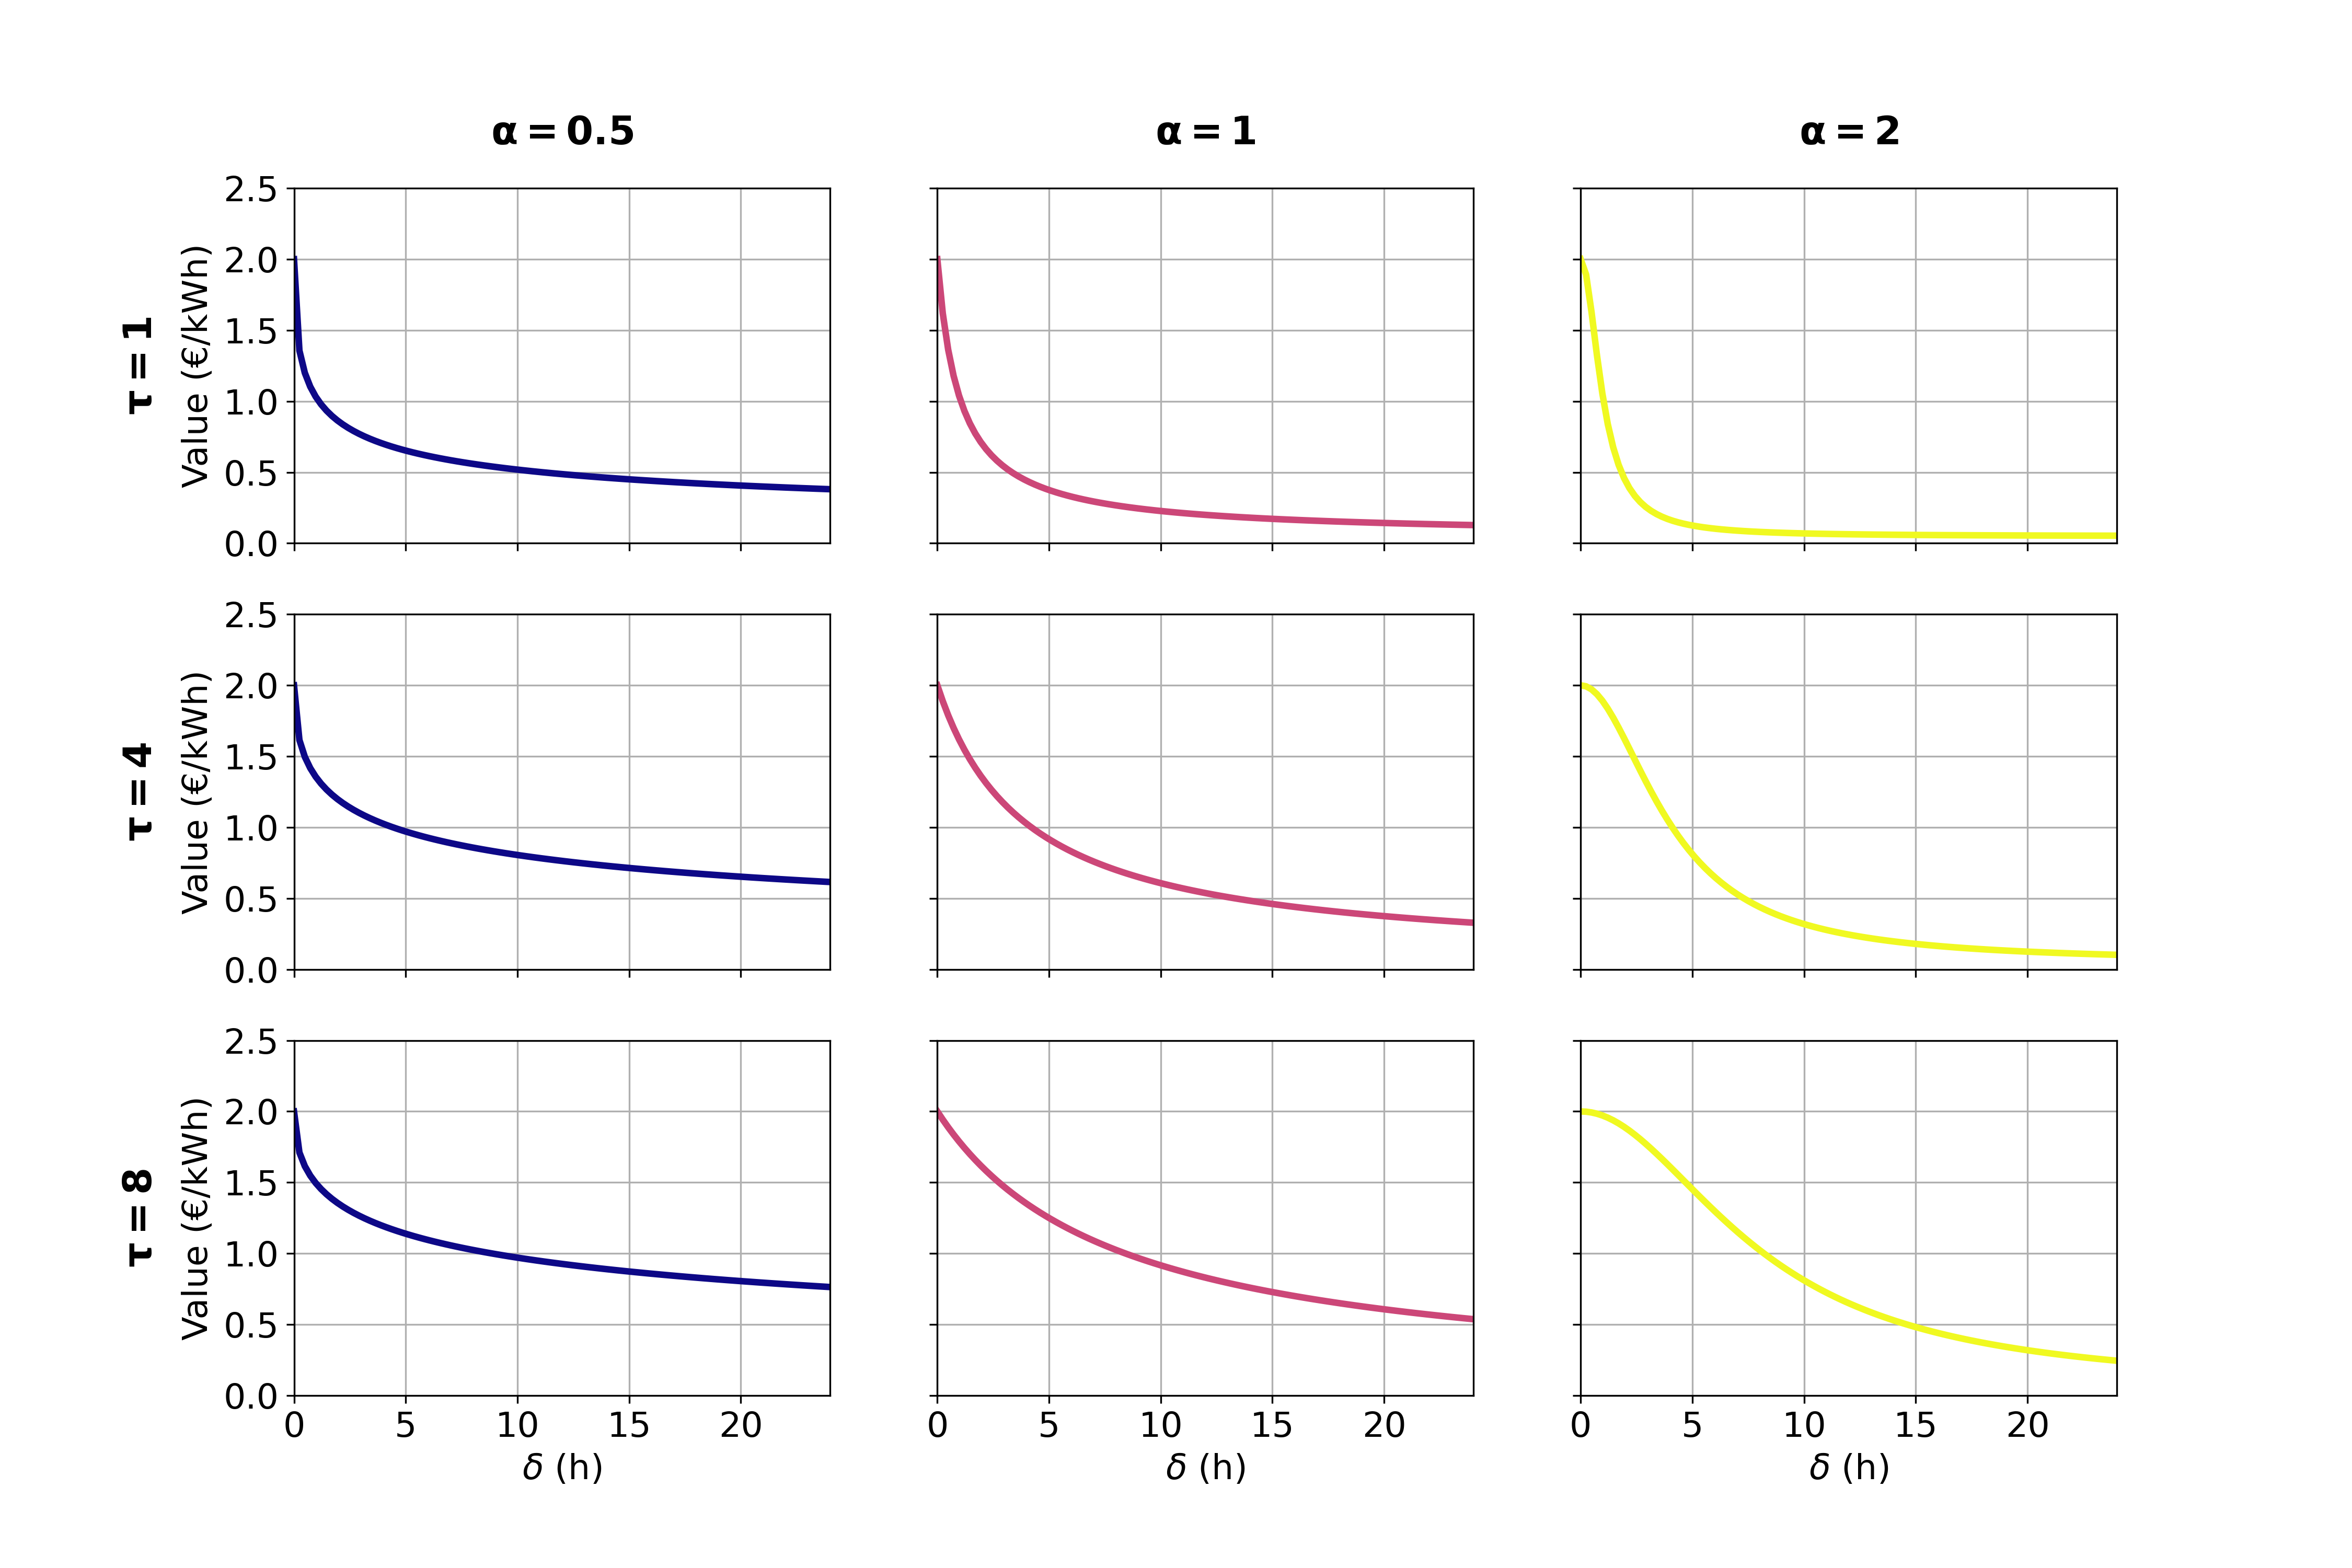
\includegraphics[width=14cm]{flexibility_value_function_color.png}
    \caption{Illustration of the flexibility value as a function of notification period \( \delta \) for different combinations of the parameters $\tau$ and $\alpha$.}
    \label{fig:flex_value_vs_time}
\end{figure}

The shape of the curve defined by equation \ref{smooth_decay} captures the relationship between the notification period \( \delta \) and the economic value of flexibility. Physically, the left endpoint of the curve at \( \delta = 0 \) corresponds to real-time or near-immediate activation. The value at this point is set to \( V_{\max} \), representing the upper bound of compensation, typically aligned with the remuneration for short-term balancing services such as Frequency Containment Reserve (FCR), automatic Frequency Restoration Reserve (aFRR), or mFRR ~\cite{entsoe_balancing}. Conversely, for longer notice periods, the flexibility value decreases and converges toward \( V_{\min} \), reflecting prices found in markets where scheduling less time-sensitive.

This is shown in Fig.~\ref{fig:flex_value_vs_time}, where the effects of different values of \( \tau \) and \( \alpha \) are illustrated. By exploring a range of these parameters, the robustness of the proposed bidding strategy can be assessed under different assumptions about aggregator behavior and market price dynamics.

The values of \( V_{\max} \) and \( V_{\min} \) are therefore selected based on representative market data. For example, \( V_{\max} \) can be calibrated to reflect historical average activation prices in FCR or mFRR markets (e.g., 200–300 \texteuro/MWh), while \( V_{\min} \) may correspond to average day-ahead prices or avoided energy costs (e.g., 50–70 \texteuro/MWh). These ranges ensure that the flexibility valuation remains grounded in practical operational conditions while allowing sensitivity analysis through the tunable parameters \( \tau \) and \( \alpha \). For the purposes of this study, the analysis is carried out setting $V_{\max} = 2$~\texteuro/kWh and $V_{\min} = 0.05$~\texteuro/kWh. These values are selected to span the range of compensation observed across electricity market products. $V_{\min}$ represents lower-value flexibility opportunities, such as day-ahead energy price levels or avoided energy costs, consistent with average clearing prices observed in Iberian and Central European day-ahead markets. $V_{\max}$ represents an upper-bound remuneration level associated with near-immediate activation under scarcity-driven balancing conditions. It should not be interpreted as an average balancing price, but rather as a ceiling value capturing high-value system-stress scenarios; analysis of European balancing activation prices confirms that scarcity-driven mFRR activations can reach price levels of this order of magnitude~\cite{entsoe_balancing}. This parametrization allows $V(\delta)$ to span the full range from routine energy arbitrage to premium short-notice response. While the bounds $V_{\max}$ and $V_{\min}$ are empirically informed, the intermediate decay profile of $V(\delta)$ is not uniquely determined from available market data. The parameters $\tau$ and $\alpha$ are therefore varied parametrically to represent different rates at which flexibility value may decrease with notification time, enabling a structured sensitivity analysis under alternative assumptions regarding aggregator preferences and market time-sensitivity.



\section{Results}\label{results}
%Describe what will be presented in the results section in a small PAR


\subsection{"A posteriori" flexibility assessment} \label{a_posteriori_results}

To assess the inherent flexibility within the DC workload, estimated GPU-side power is disaggregated by task latency classes as defined in Section~\ref{a_posteriori}. Two sets of latency classes are chosen to characterize the latency distribution of the DC power trace and to explore the potential for demand-side flexibility.

\begin{figure}[!h]
    \centering

    \begin{subfigure}[b]{0.9\textwidth}
        \centering
        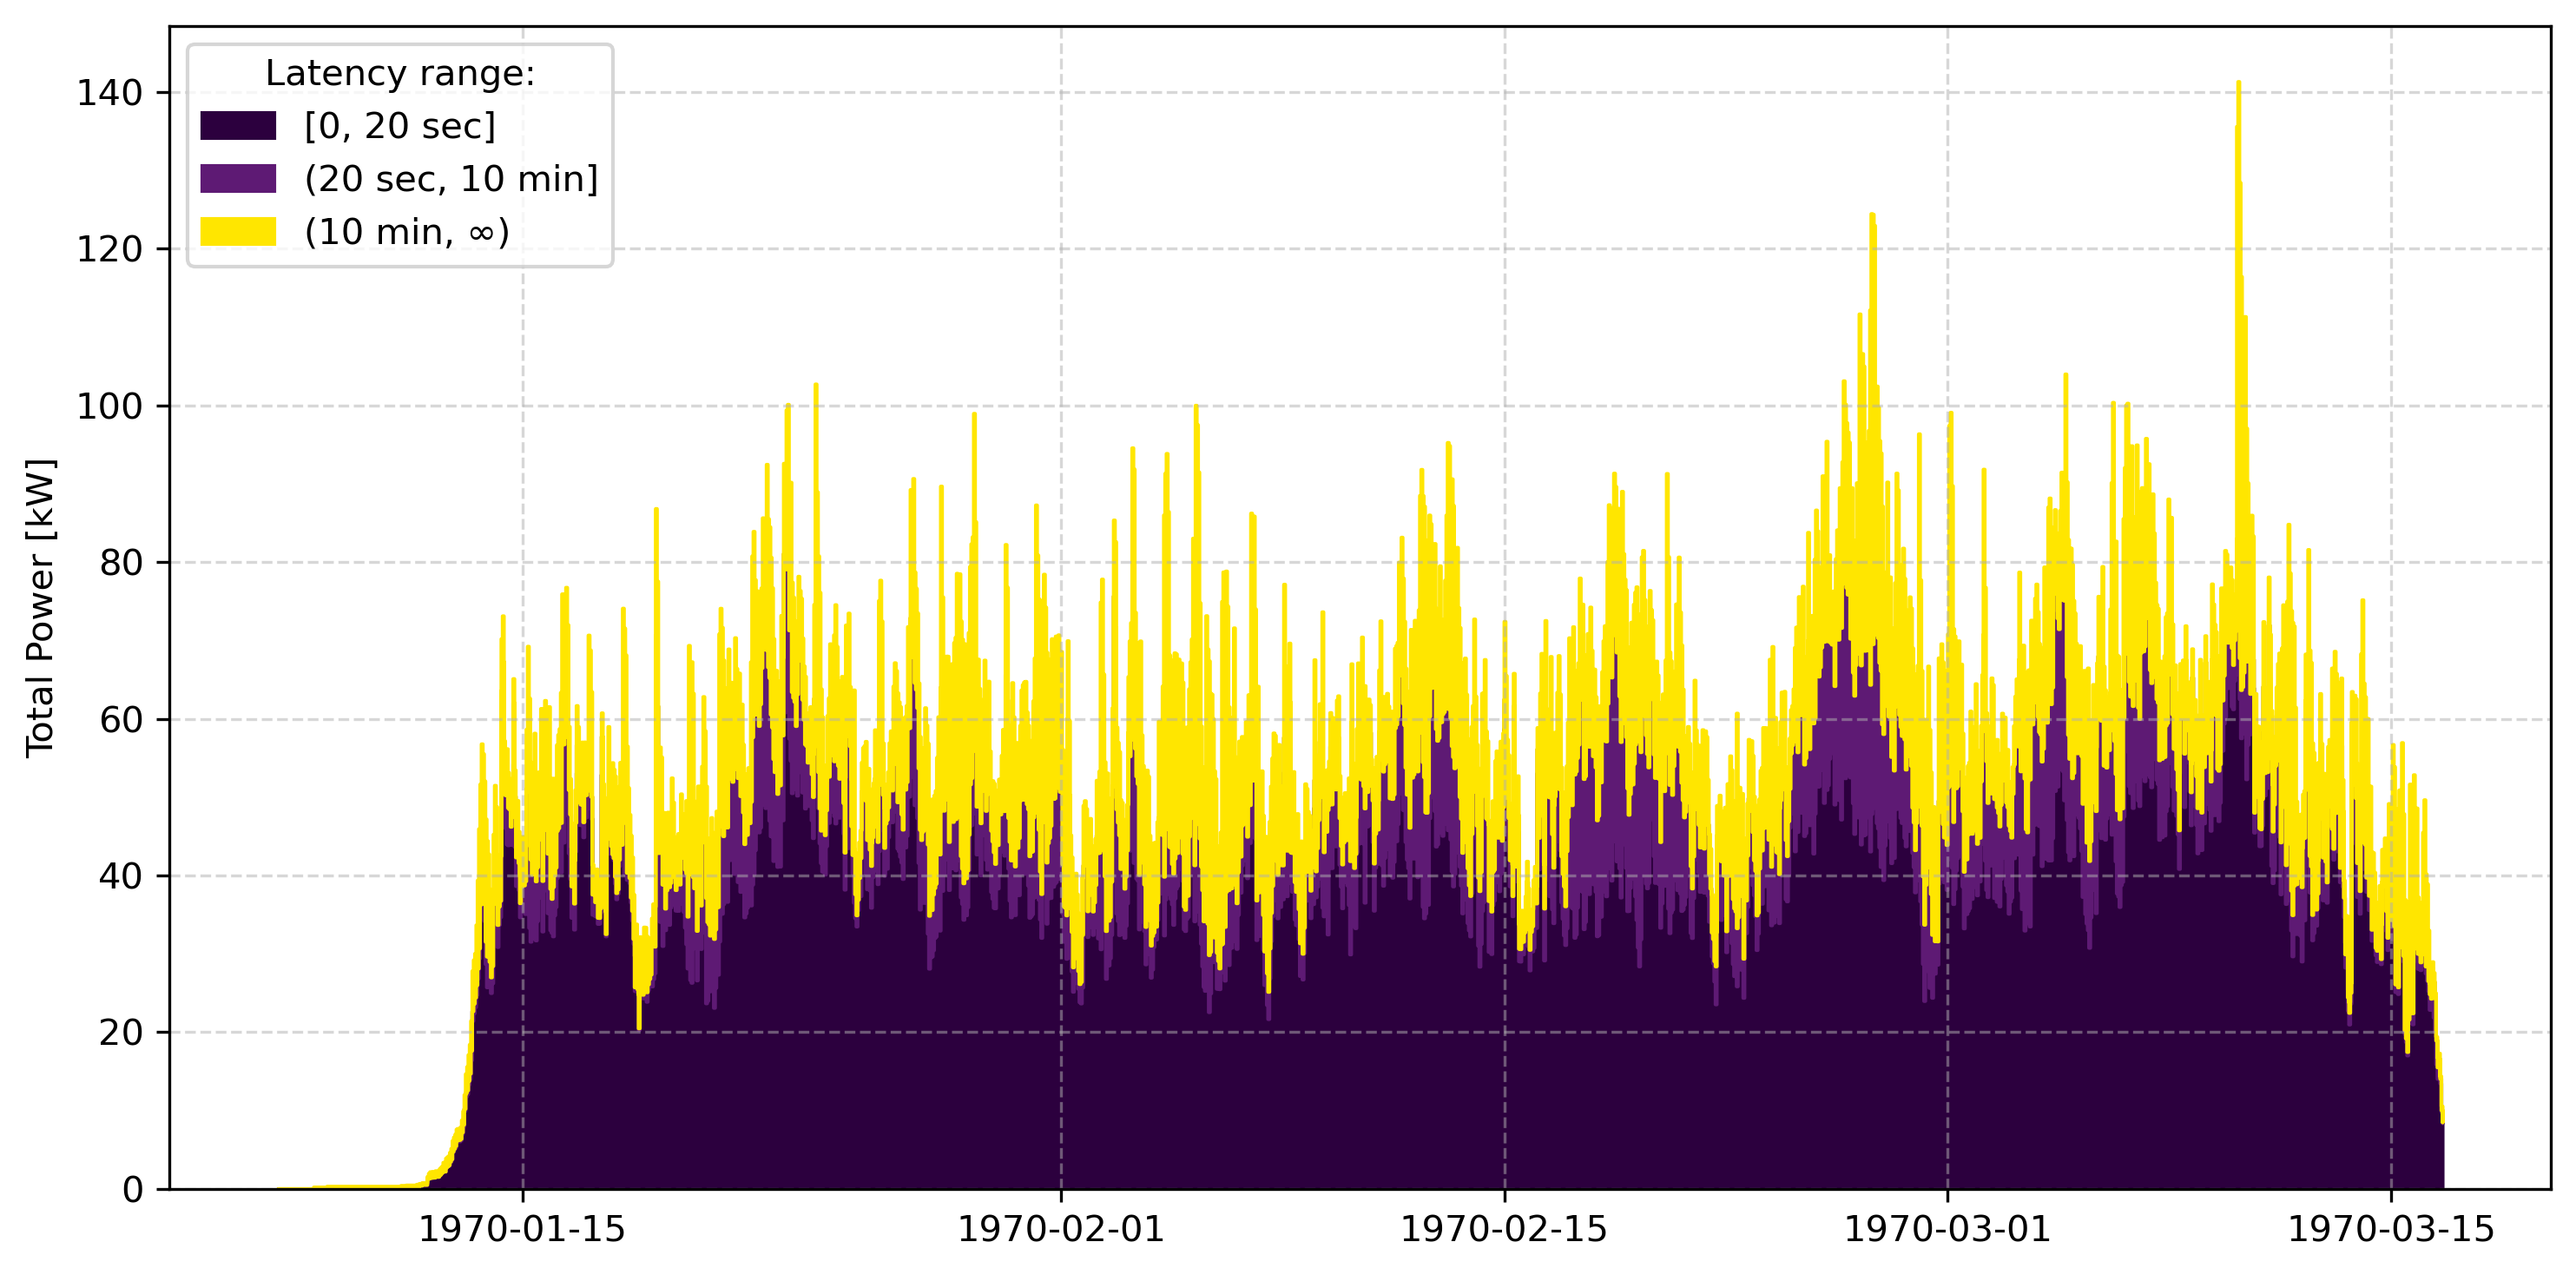
\includegraphics[width=\linewidth]{a_posteriori_interval1.png}
        \caption{}
        \label{fig:interval_1a}
    \end{subfigure}

    \vspace{0.5cm} % optional spacing between images

    \begin{subfigure}[b]{0.9\textwidth}
            \centering
        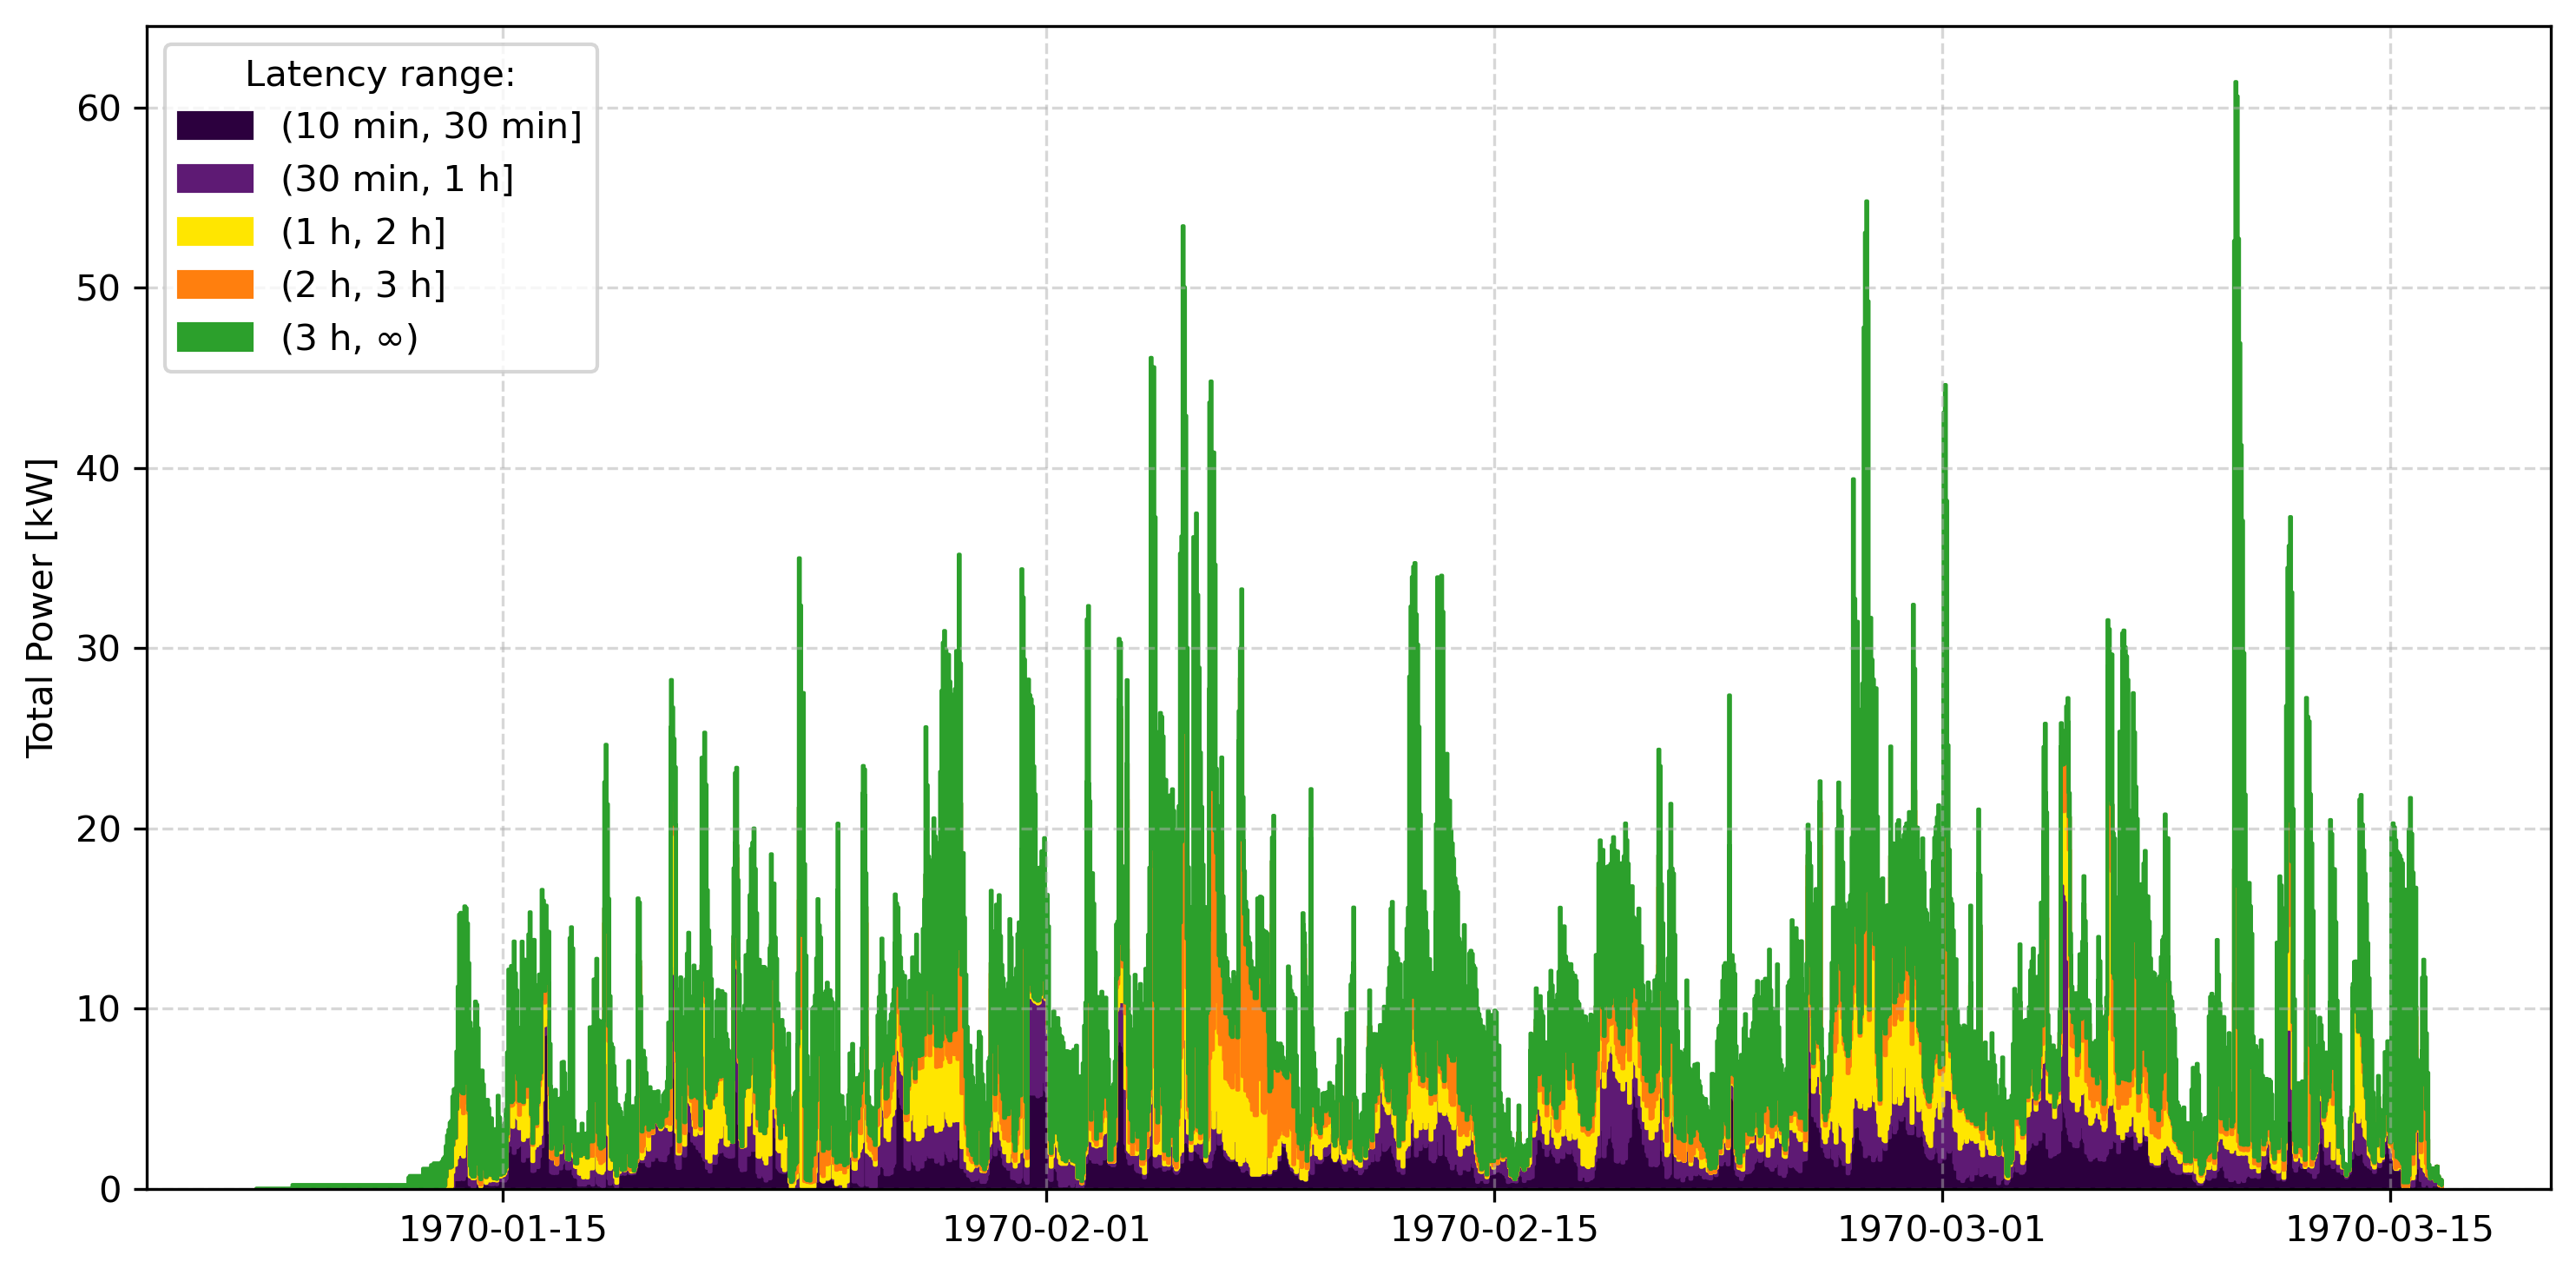
\includegraphics[width=\linewidth]{a_posteriori_interval2.png}
        \caption{}
        \label{fig:interval_1b}
    \end{subfigure}

    \caption[Latency overview]{Stacked time series of estimated GPU-side power categorized by latency ranges: (a) full latency range, (b) focus on flexible latency range only.}
    \label{fig:interval_comparison}
\end{figure}

\begin{table}[h!]
\centering
\renewcommand{\arraystretch}{1.3}
\begin{tabular}{@{} >{\centering\arraybackslash}m{4cm} c cc c cc @{}}
\toprule
\textbf{Latency Range} 
& & \multicolumn{2}{c}{\textbf{Tasks}} 
& \multicolumn{1}{c}{} 
& \multicolumn{2}{c}{\textbf{Average Power}} \\
\cmidrule(lr){3-4} \cmidrule(lr){6-7}
 & & \textbf{(\%)} & \textbf{(-)} 
 & & \textbf{(\%)} & \textbf{(kW)} \\
\midrule
\textit{$[0,\ 20\,\mathrm{sec}]$}  & & 79.8 & 584381 & & 65.0 & 36.96 \\
\textit{$(20\,\mathrm{sec},\ 10\,\mathrm{min}]$}  & & 14.7 & 107720 & & 14.4 & 8.19 \\
\textit{$(10\,\mathrm{min},\ 30\,\mathrm{min}]$} & & 2.3 & 16645 & & 3.2 & 1.84 \\
\textit{$(30\,\mathrm{min},\ 1\,\mathrm{h}]$} & & 1.6 & 11479 & & 2.6 & 1.48 \\
\textit{$(1\,\mathrm{h},\ 2\,\mathrm{h}]$} & & 0.7 & 5216 & & 2.9 & 1.62 \\
\textit{$(2\,\mathrm{h},\ 3\,\mathrm{h}]$} & & 0.3 & 2075 & & 1.7 & 0.99 \\
\textit{$(3\,\mathrm{h},\ \infty)$} & & 0.7 & 5174 & & 10.1 & 5.75 \\
\bottomrule
\end{tabular}
\caption{Distribution of tasks and estimated GPU-side power across latency groups.}
\label{tab:latency_distribution}
\end{table}


Fig. \ref{fig:interval_comparison} presents the time series of total GPU power consumption, categorized by latency range. Panel (a) shows the full latency spectrum, revealing that a majority of the power consumption originates from low-latency tasks (particularly in the [0, 20 sec] and [20 sec, 10 min] categories). These tasks represent over 94\% of all jobs and account for approximately 79.4\% of total power usage, as shown in Table~\ref{tab:latency_distribution}. This suggests that a large portion of the DC workload presents low latency and offers limited flexibility for rescheduling. 

However, panel (b) isolates the higher-latency categories ($\geq$10 min), which represent a smaller share of tasks (5.5\%) but a disproportionately higher share of the estimated GPU power (over 20\%). Notably, the [3h, $\infty$) category alone contributes 10.1\% of the estimated total while comprising just 0.7\% of the workload. Although the absolute magnitudes depend on the adopted GPU power model, this result still indicates that high-latency workloads account for a meaningful share of the workload segments most relevant for flexibility assessment.

Accordingly, the power values reported in this section should be interpreted primarily as workload-level estimates for comparing flexibility potential across latency classes and time periods, rather than as hardware-calibrated measurements of physical GPU power.

This analysis highlights significant flexibility potential in the long-latency workload segment. Specifically:
\begin{itemize}
    \item Temporal shifting of tasks in the $\geq$10 min categories can help reduce peak load periods.
    \item Load shaping strategies targeting these workloads could support energy arbitrage or renewable integration.
    \item Even a modest deferral or coordination of the [3h, $\infty$) tasks can yield meaningful reductions in peak power draw due to their high individual energy intensity.
\end{itemize}

In summary, while most of the workload is constrained by tight latency requirements, a non negligible portion exhibits scheduling flexibility. Identifying this flexible power capacity could form the basis for DR mechanisms and long-term energy aware scheduling strategies in DC operations.





\subsection{LAD-Flex strategy results} \label{LAD_flex_results}

The strategy is tested for a sample week, as mentioned in Section \ref{case study}. Its execution begins when a flexibility request is issued to the DC. From that point until the end of the flexibility window, the DC continuously monitors all incoming tasks. Tasks that meet the deferrability criteria defined by LAD-Flex are deferred for execution outside the flexibility period, thereby reducing power demand during the requested interval.

The following subsections present results for three market scenarios defined in Section \ref{Case_study_scenarios}: a baseline aggregator-coordinated scenario, an intraday market scenario, and an mFRR balancing reserve scenario. For all scenarios, the ideal case of perfect task duration prediction ($\zeta = 0$) is initially considered; robustness under prediction uncertainty is analyzed separately in Section~\ref{sec:robustness}.

To gain insights into how the LAD-Flex strategy performs under different conditions, nine representative points were selected from each scenario's weekly simulation:
\begin{itemize}
    \item the three instances with the highest deferrable energy (labeled $P_1$, $P_2$, and $P_3$),
    \item three points with deferrable energy values closest to the 75th percentile ($Q_1$, $Q_2$, $Q_3$),
    \item three closest to the 50th percentile ($R_1$, $R_2$, $R_3$).
\end{itemize}

%%%%%%%%%%%%%%%%%%%%%%%%%%%%%%%%%%%%%%%%%%%%%%%%%%%%%%%%%%%%%%%%%%%%%%%%%%%%%%%
\subsubsection{Baseline Scenario} \label{baseline_scenario}
%%%%%%%%%%%%%%%%%%%%%%%%%%%%%%%%%%%%%%%%%%%%%%%%%%%%%%%%%%%%%%%%%%%%%%%%%%%%%%%

The Baseline scenario models participation in general aggregator-coordinated flexibility programs. As outlined in Section \ref{Case_study_scenarios}, this scenario serves as the reference case to present the strategy and to evaluate alternative market configurations. Table~\ref{tab:parameters_baseline} presents the LAD-Flex parameters configured for this scenario.

\begin{table}[h!]
\centering
\begin{tabular}{@{}cccccc@{}}
\toprule
\textbf{Scenario} & $\hat{\lambda}$ & $\beta_\text{overhang}$ & $\gamma_{\text{buffer}}$ & $\delta_{\text{notification}}$ & $\eta{\Delta t}$ \\ \midrule
Baseline & 10 min & 0.7 & 60 min & 60 min & 3 h \\ \bottomrule
\end{tabular}
\caption{LAD-Flex parameters for the Baseline scenario.}
\label{tab:parameters_baseline}
\end{table}

The critical latency threshold of $\hat{\lambda} = 10$~min ensures that only tasks with sufficient queuing tolerance are considered for deferral, preserving QoS for time-sensitive workloads. The notification period of $\delta_{\text{notification}} = 60$~min provides adequate time for workload replanning, while the 3 h flexibility window aligns with aggregator flexibility products. The overhang tolerance permits up to 70\% of a task's duration to extend beyond the flexibility window boundaries, and the buffer period ($\gamma_{\text{buffer}} = 60$~min) accommodates minor scheduling imperfections.

A key metric to assess the effectiveness of the strategy is the amount of energy that the DC was able to provide in the form of DR flexibility to the aggregator by deferring tasks identified by LAD-Flex. Simulating the strategy with hourly granularity for the sample week, Fig.~\ref{fig:LAD_flex_points_baseline} shows the deferrable energy for each hourly activation throughout the week.

\begin{figure}[!h]
    \centering
    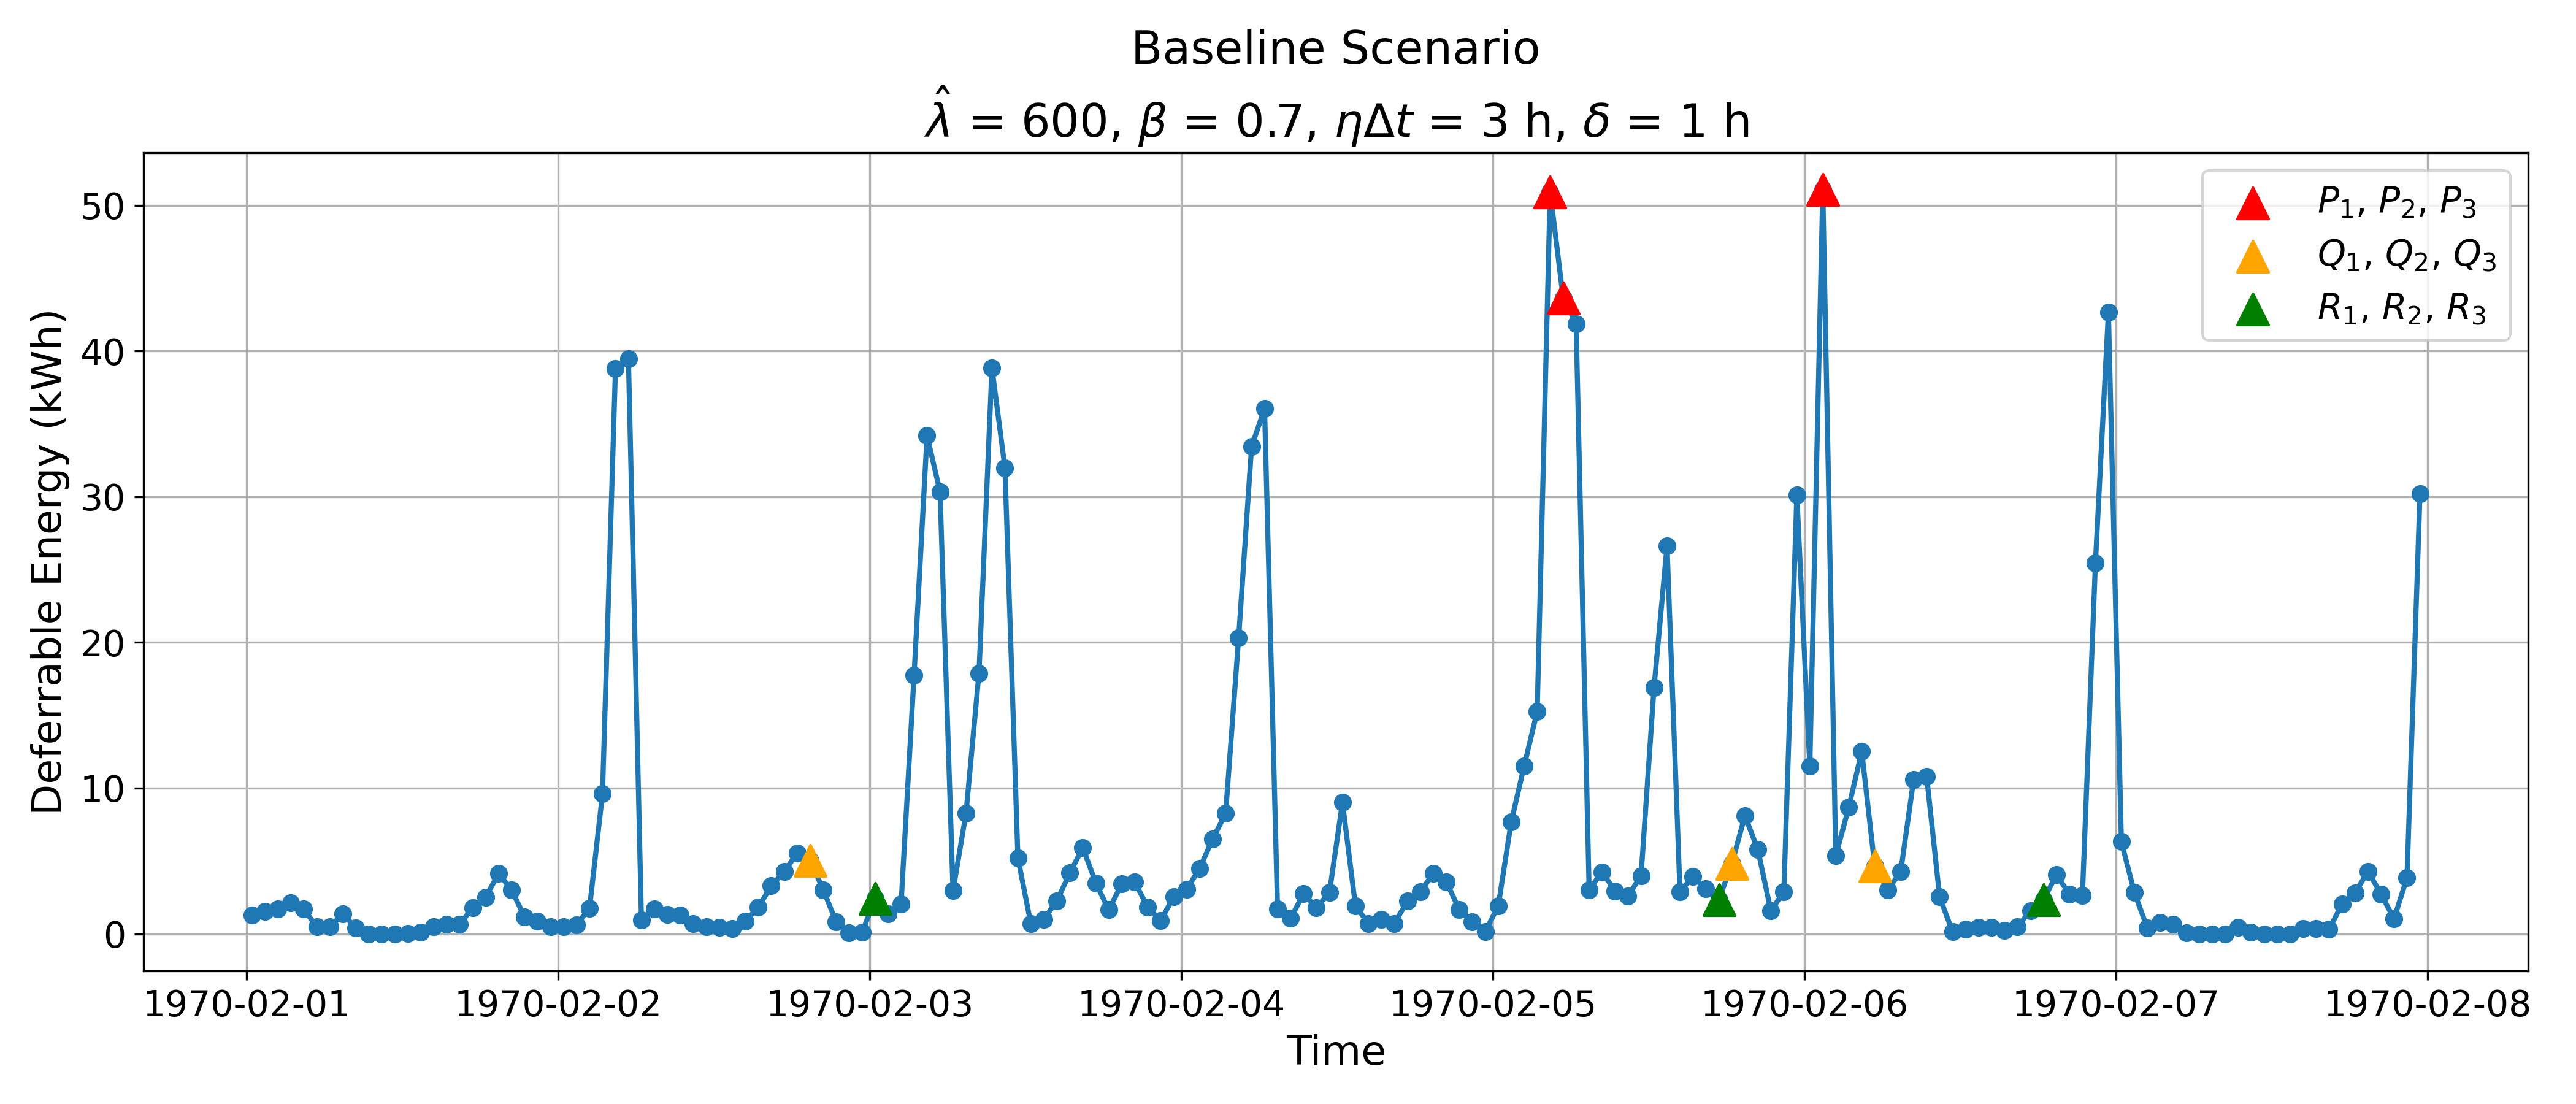
\includegraphics[width=14cm]{LARGE_DEFAULT_BASELINE_ZETA_0.png}
    \caption{Deferred energy from LAD-Flex executed hourly over the sample week for the Baseline scenario. Each point shows the deferrable energy (kWh) if a flexibility window began at that hour.}
    \label{fig:LAD_flex_points_baseline}
\end{figure}

The results reveal significant variability in flexibility potential throughout the week. Periods with concentrated non-critical workloads allow for substantial energy deferral, while other hours offer less deferrable capacity. This variability underscores the importance of aligning flexibility requests with workload characteristics to maximize impact. Fig.~\ref{fig:LAD_flex_points_grid_baseline} illustrates the LAD-Flex strategy in action for the nine selected points. At high-flexibility instances (P1–P3), the DC receives a large number of tasks meeting LAD-Flex deferrability requirements, resulting in substantial power deferral during the flexibility window. 

In contrast, during lower flexibility points (R1–R3), fewer suitable tasks are available. Nevertheless, the strategy still succeeds in deferring some energy, demonstrating that the DC can provide flexibility even under less favorable workload conditions, and viable potential for implementations at higher scales. Importantly, the overhang and buffer parameters ensure that task execution beyond the flexibility window remains minimal, preserving alignment with the aggregator's request. In most cases, the ramping of deferred power coincides with the beginning of the flexibility window, indicating that the strategy is effectively responsive to real-time activation signals, within the constraints of task arrival times.

\begin{figure}[!h]
    \centering
    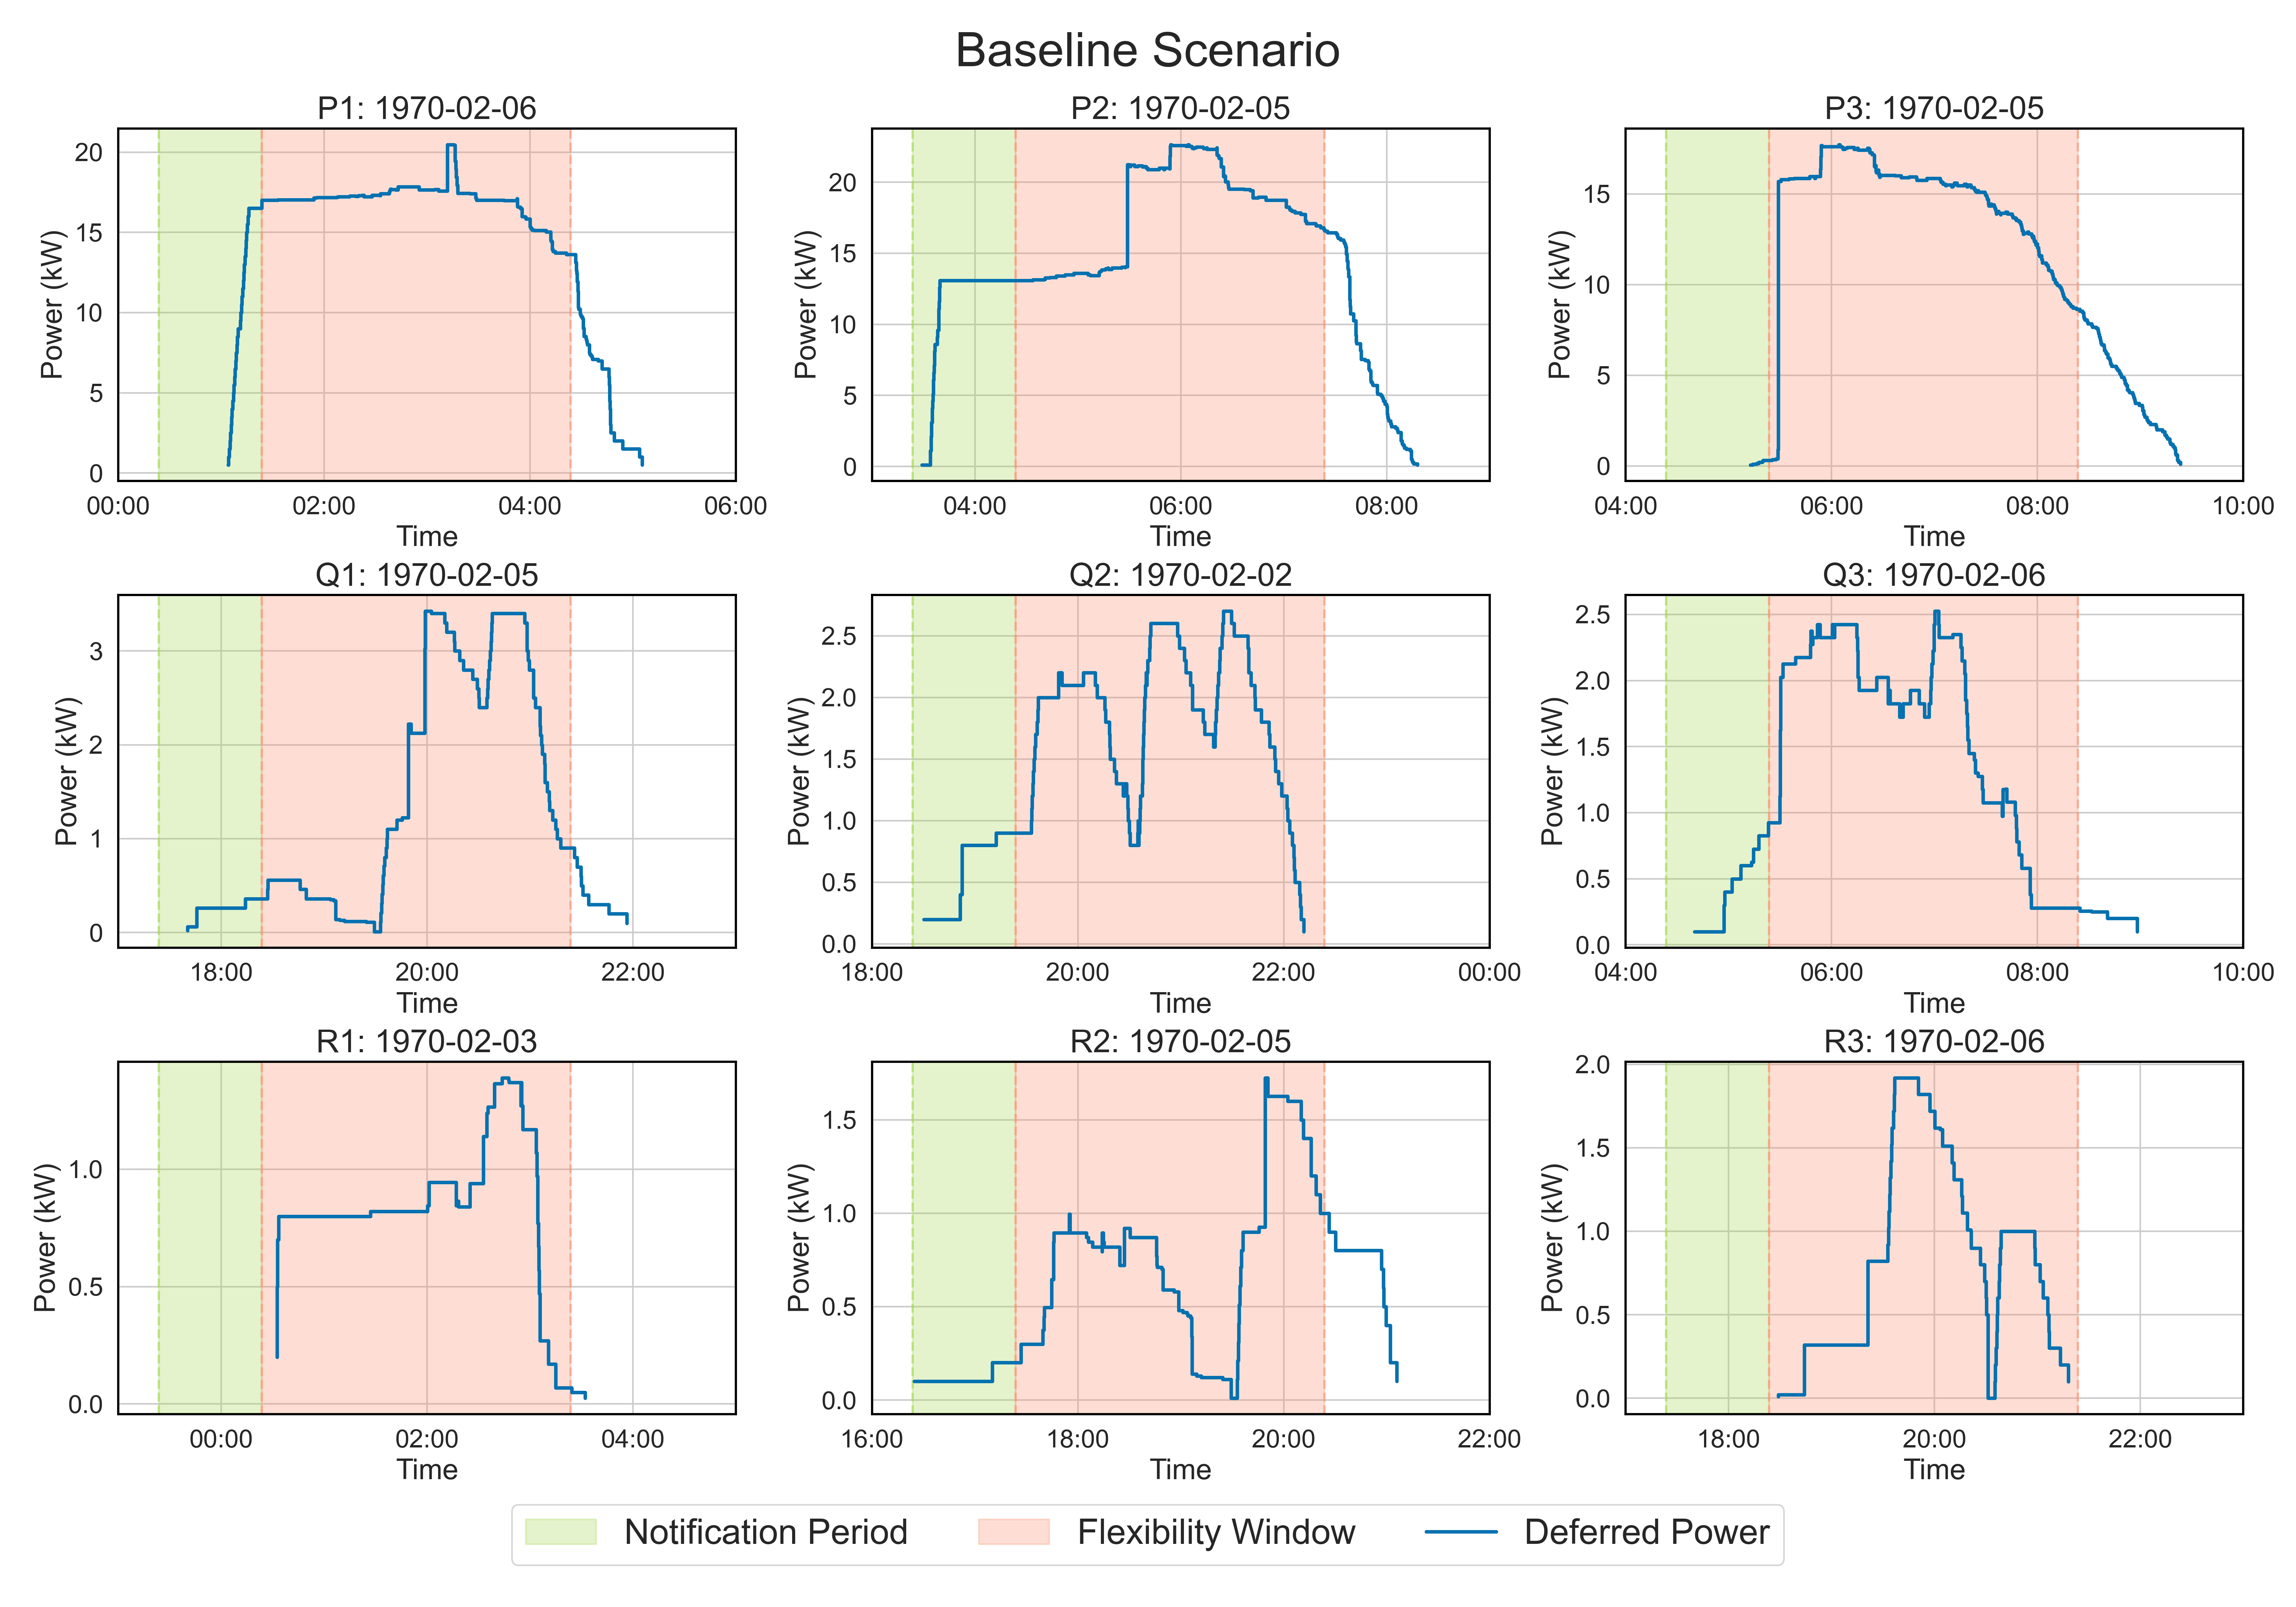
\includegraphics[width=14cm]{power_consumption_3x3_LARGE_DEFAULT_BASELINE.png}
    \caption{Deferred power profiles for LAD-Flex activations under the Baseline scenario for the 9 selected instants.}
    \label{fig:LAD_flex_points_grid_baseline}
\end{figure}

Fig.~\ref{fig:LAD_flex_summary_baseline} illustrates the estimated GPU-side power profile of the modeled IT workload before and after applying the LAD-Flex strategy at point P1. The original IT-side power demand is shown in blue, while the adjusted consumption after task deferral is depicted in purple. The green shaded area highlights the flexible energy successfully deferred during the flexibility window $[t_1, t_2]$, which was made available to the aggregator. The regions shaded in blue represent the rebound energy (i.e., corresponding to those portions of deferred tasks lying outside of the flexibility window). While this rebound does not contribute to real-time grid balancing, it is an inevitable consequence of flexibility activation. These profiles represent the direct IT-side response of LAD-Flex; any whole-facility reduction and associated PUE behavior would additionally depend on how cooling and auxiliary loads respond during the activation window, which is not observed in the trace.

\begin{figure}[!h]
    \centering
    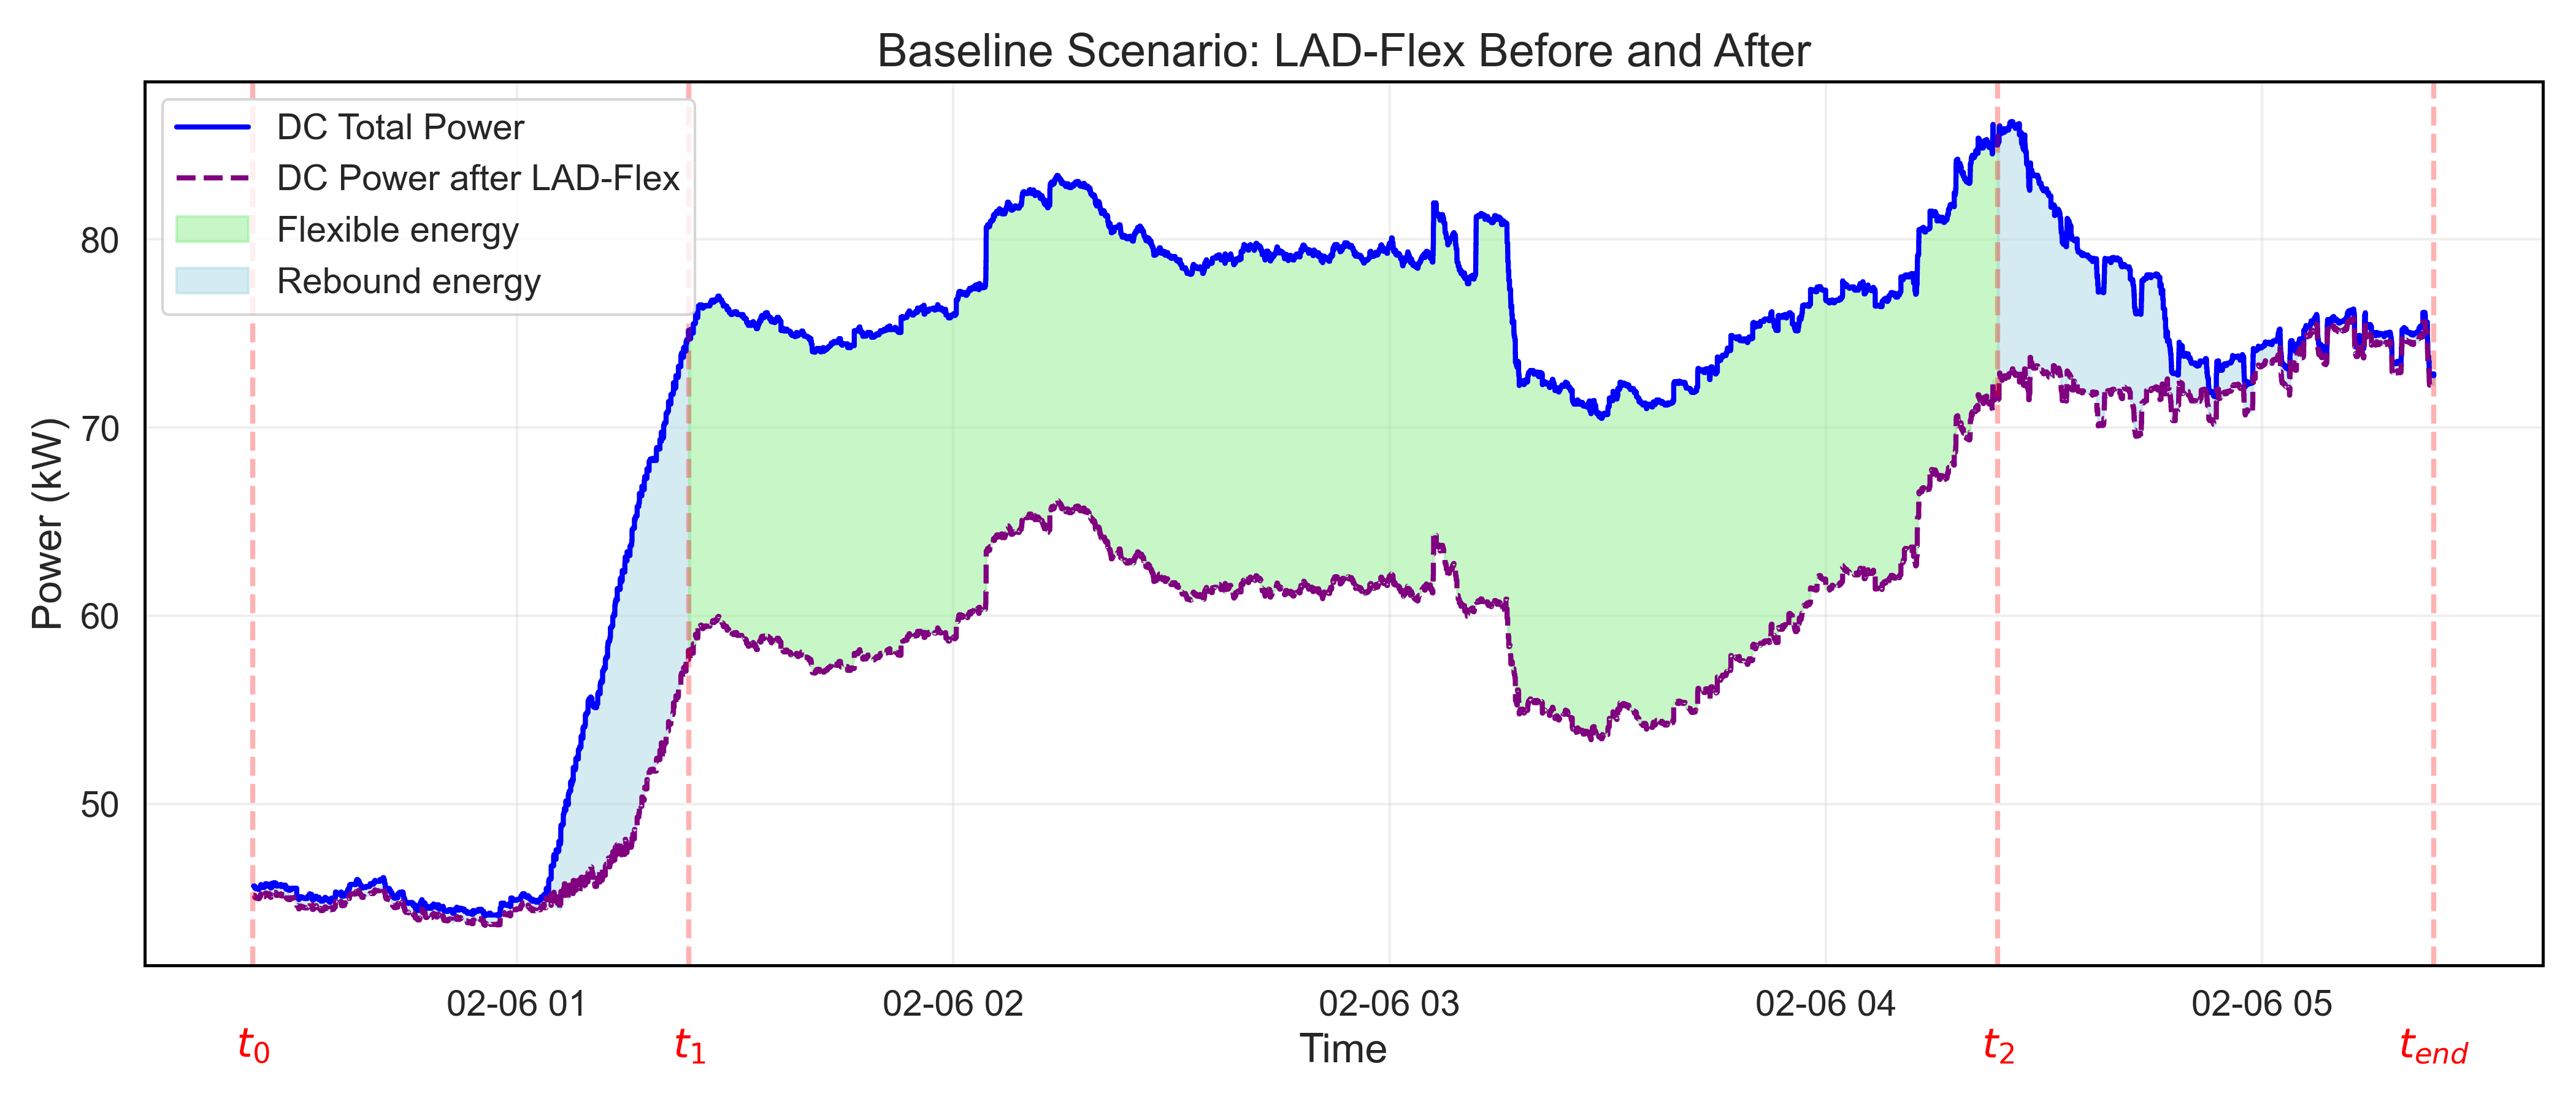
\includegraphics[width=14cm]{LAD_flex_P1_explanation_DEFAULT_BASELINE.png}
    \caption{Estimated GPU-side power of the modeled IT workload before and after LAD-Flex activation for point P1 under the Baseline scenario.}
    \label{fig:LAD_flex_summary_baseline}
\end{figure}

Table~\ref{tab:energy_flexibility_baseline} summarizes key metrics for the selected points. Points P1–P3 show both the largest number of tasks and the greatest share of deferrable energy, with over 15\% of energy shifted. Points Q1–Q3 display lower but still notable flexibility (2–3.5\%), demonstrating that LAD-Flex can consistently identify deferrable loads even under moderate activity levels. Finally, points R1–R3, closest to the median of the deferred energy distribution, yield lower deferral percentages (1.3–1.5\%).

The results show that flexibility potential is strongly influenced by workload-related characteristics. This suggests that integrating insights from LAD-Flex into the DC's scheduling decisions could enhance its ability to participate in DR programs more effectively.

\begin{table}[h!]
\centering
\renewcommand{\arraystretch}{1.2}
\begin{tabular}{@{}lrr rrr@{}}
\toprule
\textbf{Point} & \multicolumn{1}{c}{\textbf{Tasks}} & \multicolumn{3}{c}{\textbf{Energy}} \\
              & \textbf{Count} & \textbf{Deferrable (kWh)} & \textbf{Total (kWh)} & \textbf{Percentage Def. (\%)} \\
\midrule
P1 & 83  & 51.08 & 232.14 & 22.08 \\
P2 & 151 & 50.93 & 273.19 & 18.64 \\
P3 & 229 & 43.66 & 279.92 & 15.60 \\
Q1 & 56  & 4.83  & 159.14 & 3.03  \\
Q2 & 54  & 5.02  & 144.50 & 3.47  \\
Q3 & 43  & 4.66  & 189.17 & 2.46  \\
R1 & 21  & 2.41  & 159.28 & 1.51  \\
R2 & 46  & 2.34  & 174.47 & 1.34  \\
R3 & 27  & 2.32  & 171.71 & 1.35  \\
\bottomrule
\end{tabular}
\caption{Breakdown of task and energy flexibility by point for the Baseline scenario.}
\label{tab:energy_flexibility_baseline}
\end{table}


%%%%%%%%%%%%%%%%%%%%%%%%%%%%%%%%%%%%%%%%%%%%%%%%%%%%%%%%%%%%%%%%%%%%%%%%%%%%%%%
\subsubsection{Intraday Market Scenario} \label{intraday_scenario}
%%%%%%%%%%%%%%%%%%%%%%%%%%%%%%%%%%%%%%%%%%%%%%%%%%%%%%%%%%%%%%%%%%%%%%%%%%%%%%%

The intraday market scenario reflects participation in continuously coupled intraday electricity markets, where flexibility requests are issued several hours before delivery to balance portfolios and optimize market positions. This scenario features longer flexibility windows and notification periods compared to the baseline. Table~\ref{tab:parameters_intraday} presents the LAD-Flex parameters configured for this scenario.

\begin{table}[h!]
\centering
\begin{tabular}{@{}cccccc@{}}
\toprule
\textbf{Scenario} & $\hat{\lambda}$ & $\beta_\text{overhang}$ & $\gamma_{\text{buffer}}$ & $\delta_{\text{notification}}$ & $\eta{\Delta t}$ \\ \midrule
Intraday & 30 min & 0.9 & 120 min & 3 h & 4 h \\ \bottomrule
\end{tabular}
\caption{LAD-Flex parameters for the intraday market scenario.}
\label{tab:parameters_intraday}
\end{table}

The extended flexibility window ($\eta{\Delta t} = 4$~h) and longer notification period ($\delta_{\text{notification}} = 3$~h) allow the DC to accumulate more deferrable tasks over a wider time horizon. The increased latency threshold ($\hat{\lambda} = 30$~min) ensures that only less time-sensitive tasks are selected for deferral. Additionally, the higher overhang parameter ($\beta_{\text{overhang}} = 0.9$) permits tasks with longer expected durations to be deferred and the extended buffer period ($\gamma_{\text{buffer}} = 120$~min) provides additional margin for task completion.

Fig.~\ref{fig:LAD_flex_points_intraday} shows the deferrable energy for each hourly activation throughout the sample week. Compared to the Baseline scenario, the Intraday configuration yields higher peak flexibility volumes per activation, with maximum deferrable energy exceeding 100~kWh. This increase is attributed to the longer flexibility window, which captures more tasks eligible for deferral, and the extended notification period, which allows the strategy to begin monitoring incoming tasks earlier, despite the higher value of critical latency.

\begin{figure}[!h]
    \centering
    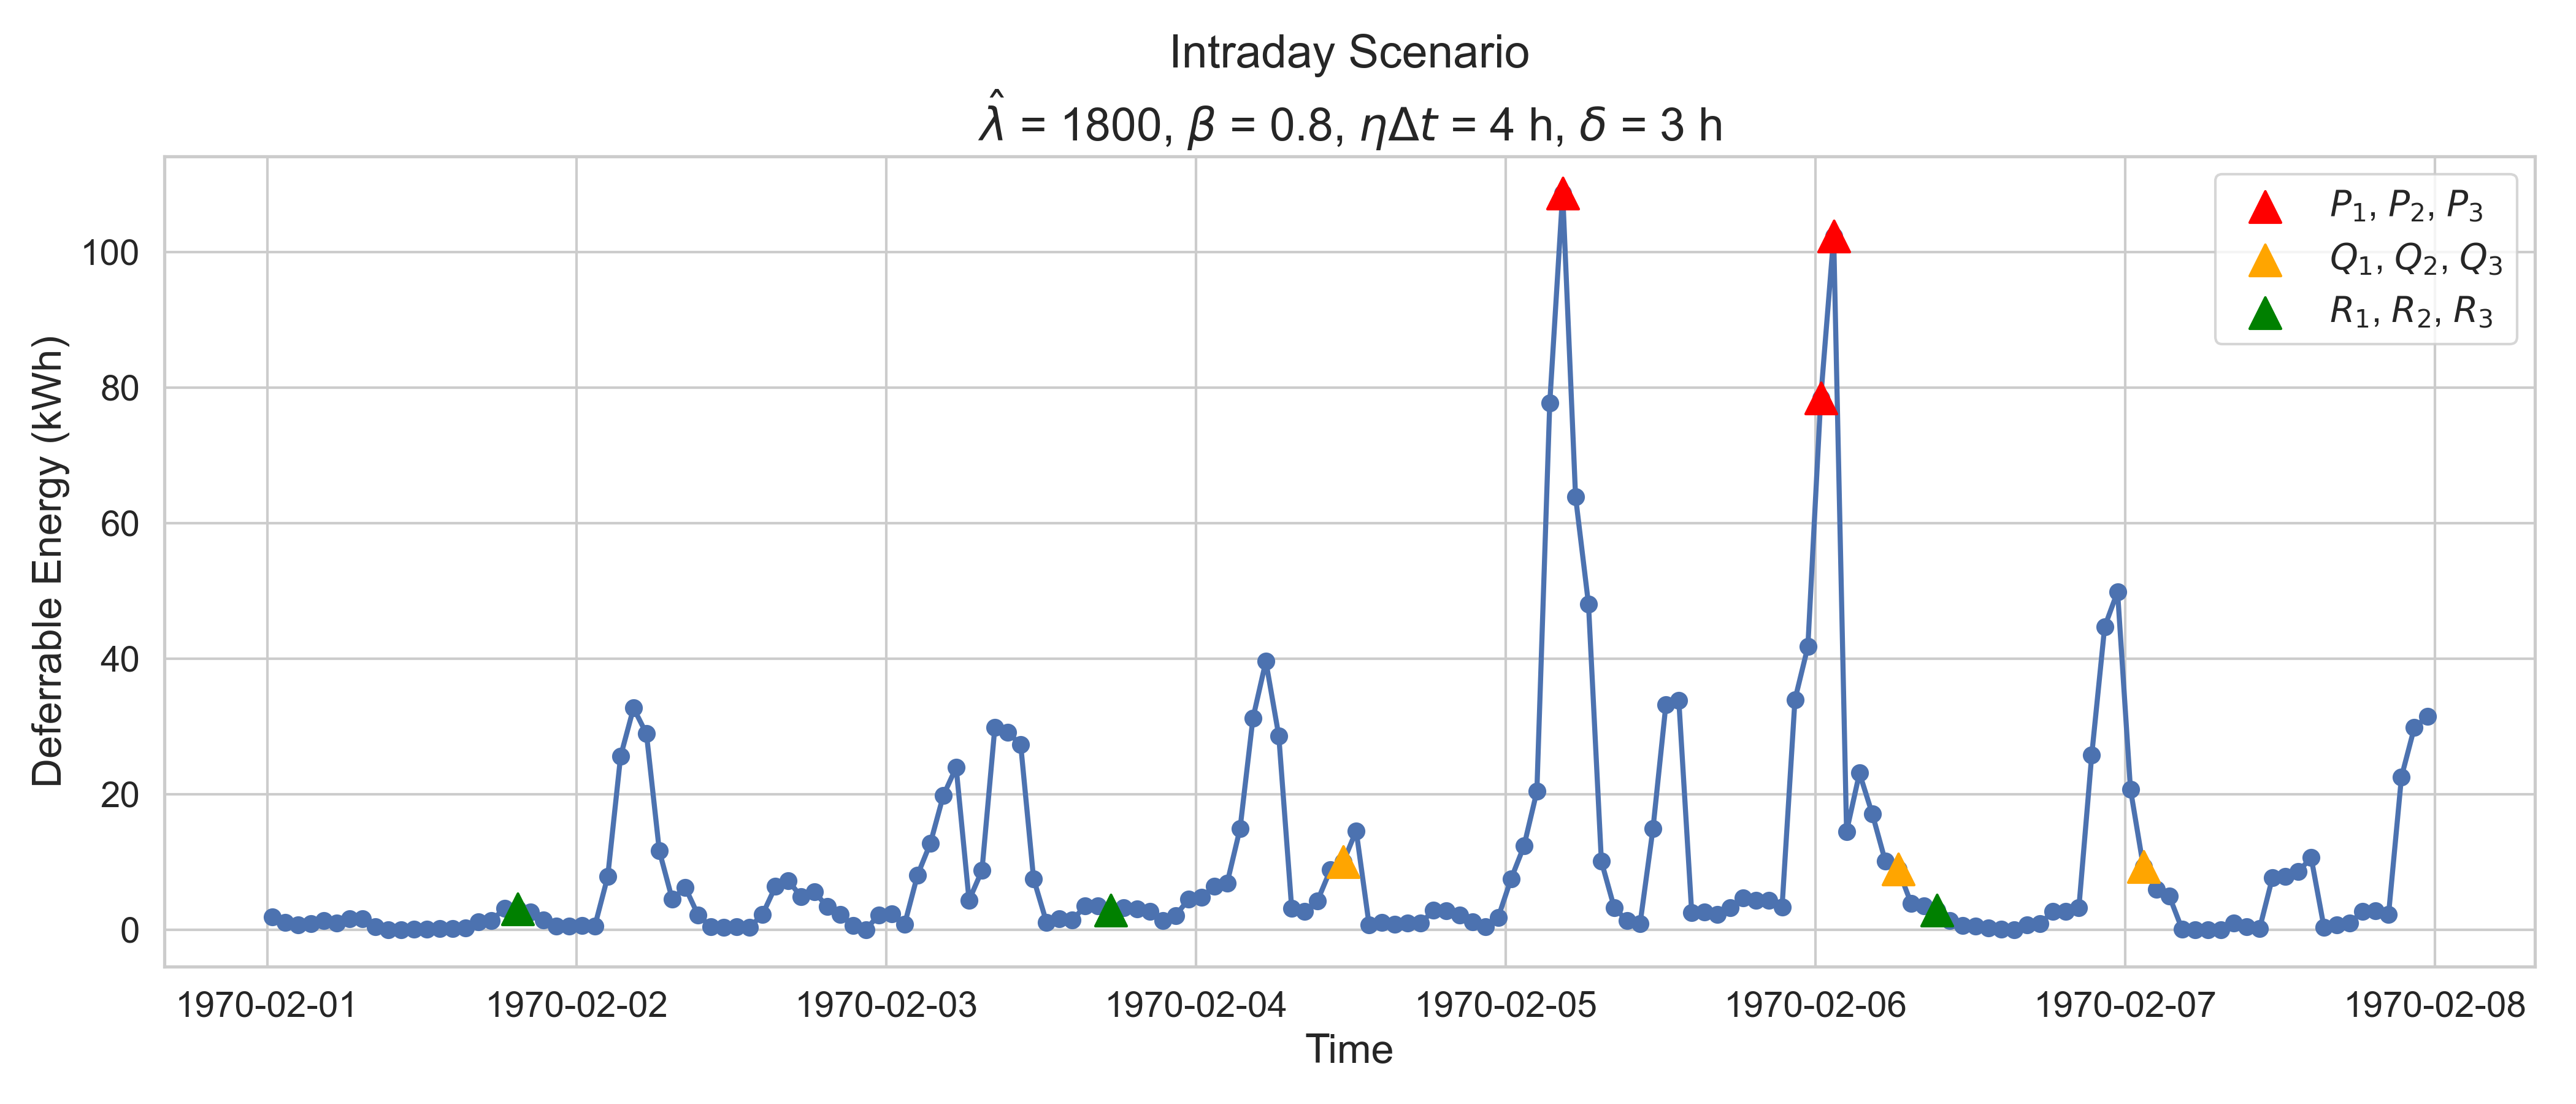
\includegraphics[width=14cm]{LARGE_DEFAULT_DAM_ZETA_0.png}
    \caption{Deferred energy from LAD-Flex executed hourly over the sample week for the Intraday scenario.}
    \label{fig:LAD_flex_points_intraday}
\end{figure}

Fig.~\ref{fig:LAD_flex_points_grid_intraday} illustrates the deferred power profiles for the nine selected points. The extended flexibility window is clearly visible in all subplots, with the deferred power maintained over a 4-hour period. At high-flexibility instances (P1–P3), deferred power reaches values above 25–35~kW, with P1 showing a sustained deferral profile that peaks around 35~kW. The longer notification period allows the strategy to begin accumulating deferrable tasks earlier, resulting in smoother power profiles compared to the Baseline scenario. For the mid-range points (Q1–Q3), deferred power stabilizes around 2–3~kW, while the median points (R1–R3) show lower but consistent deferral in the range of 1–2~kW. Notably, even at these lower flexibility instances, the strategy successfully maintains load reduction throughout the entire flexibility window, demonstrating the reliability of LAD-Flex under varying workload conditions.

\begin{figure}[!h]
    \centering
    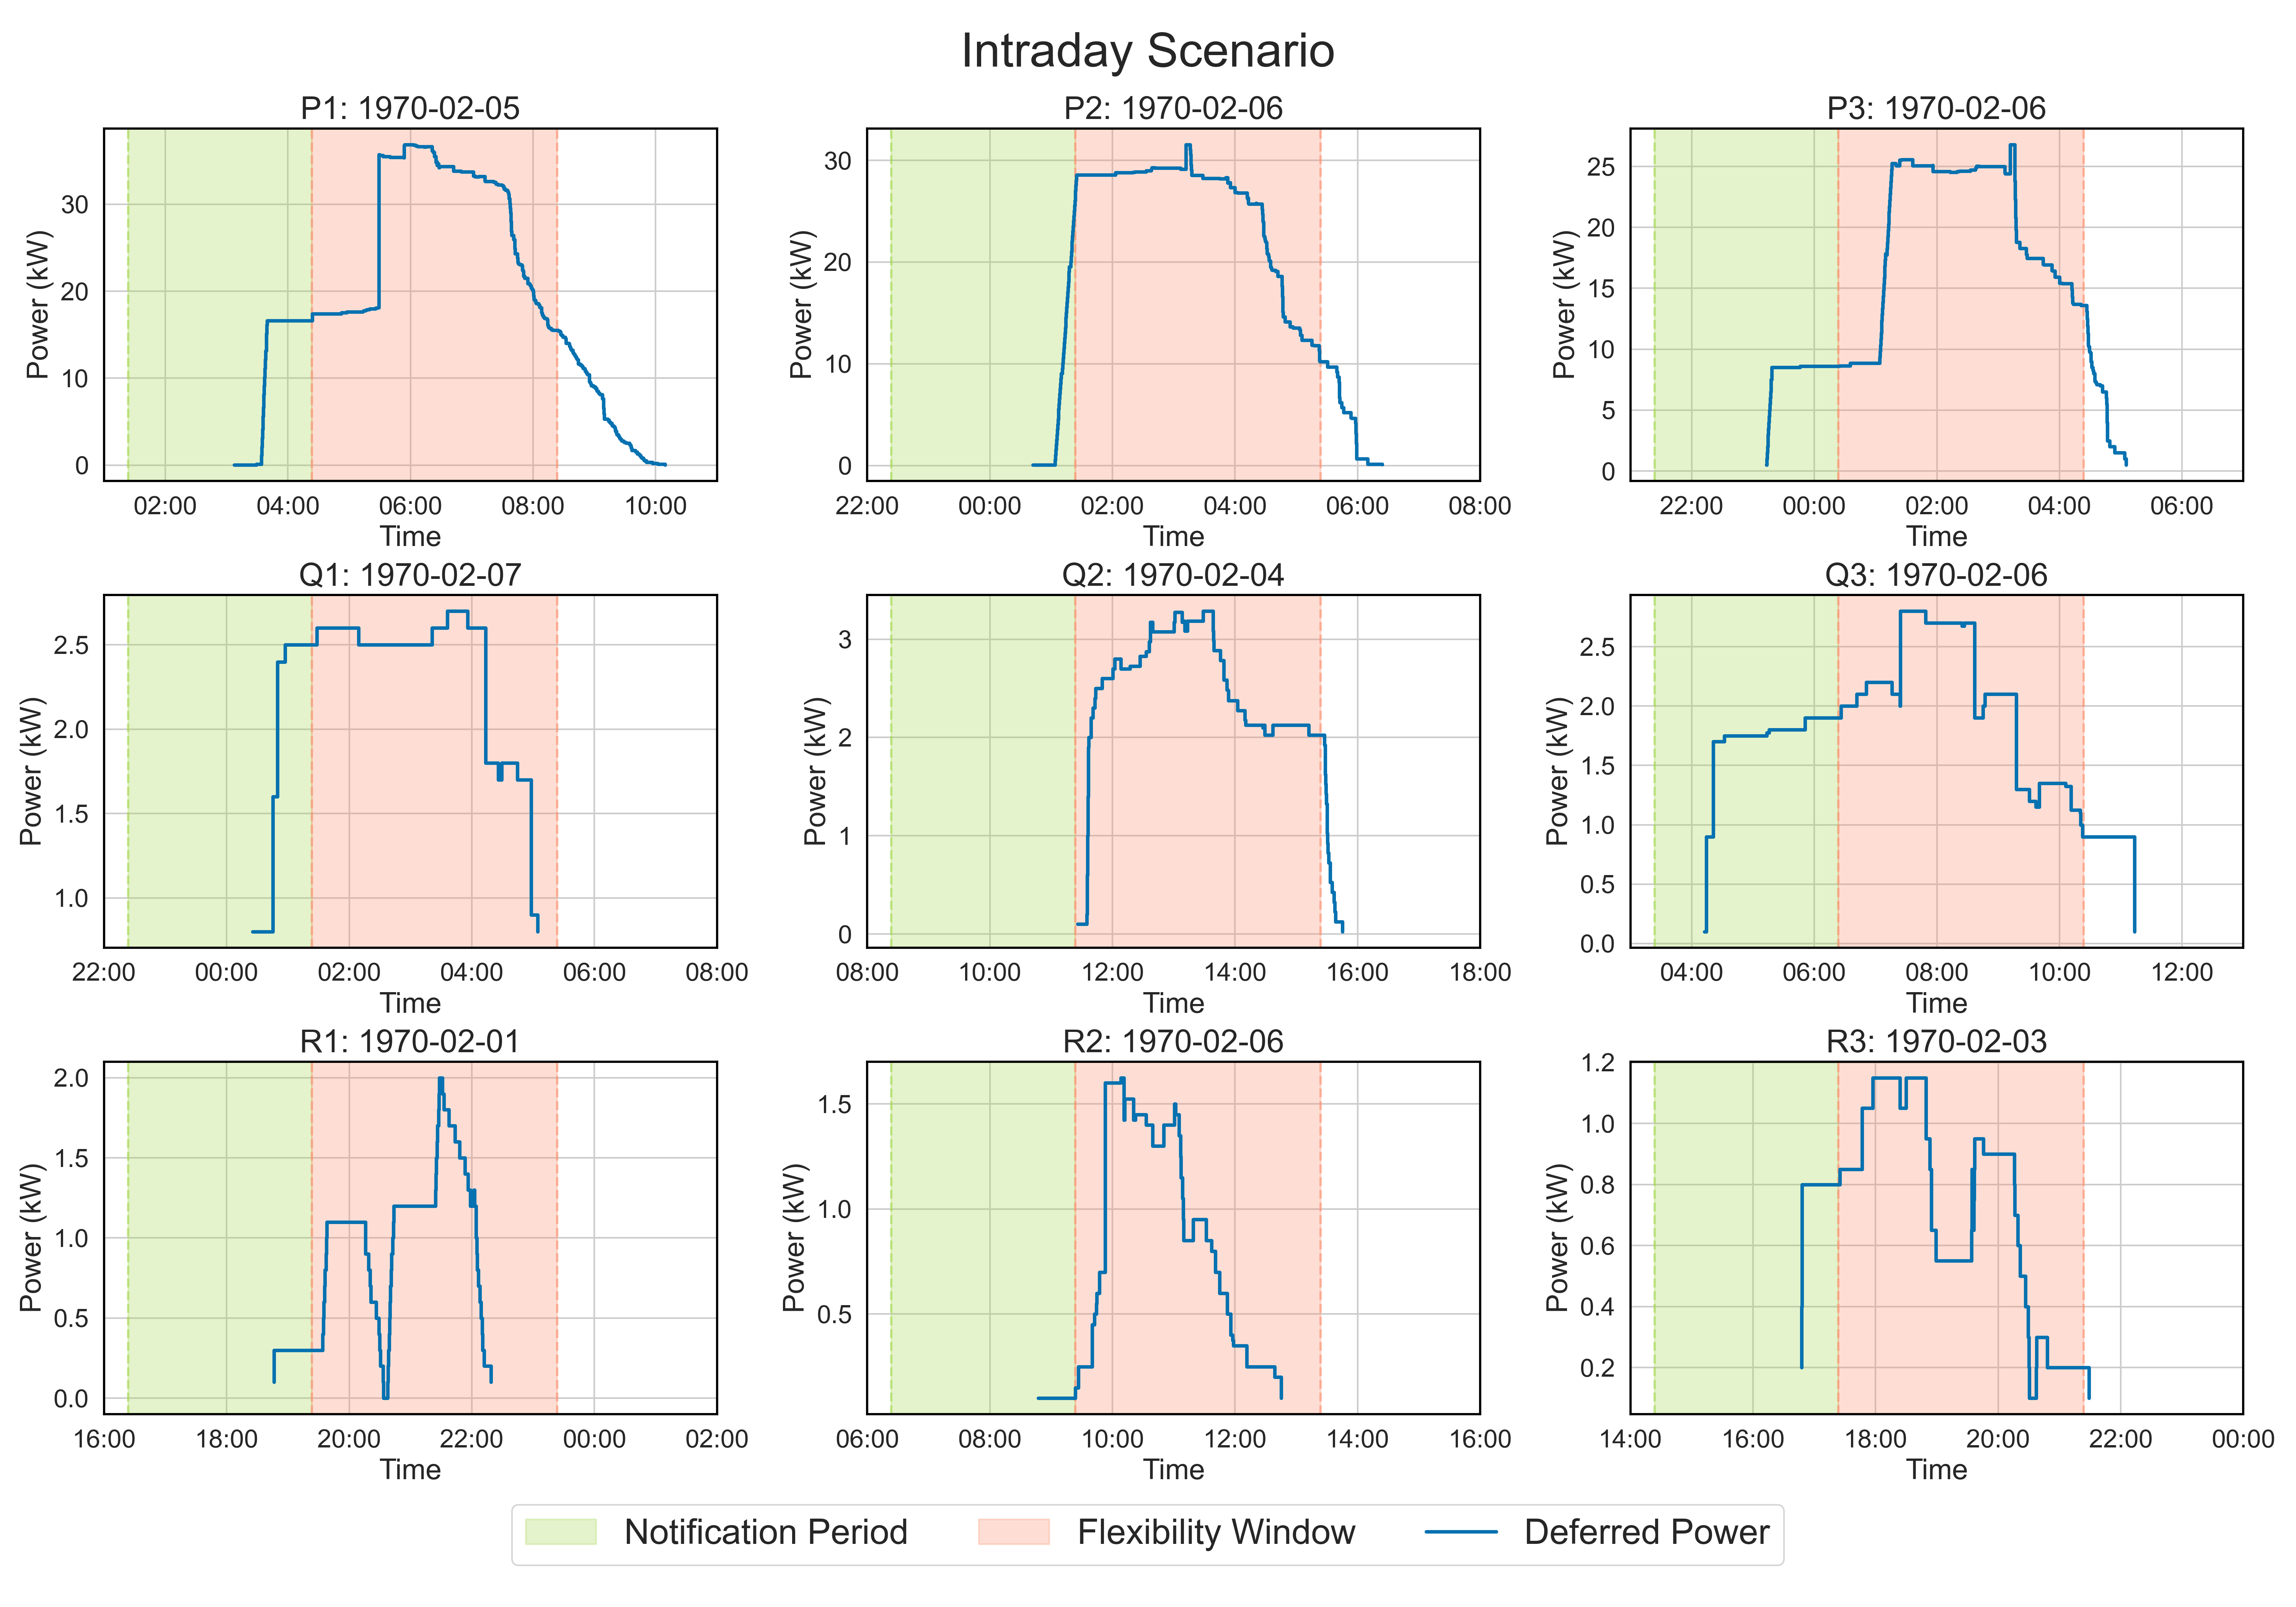
\includegraphics[width=14cm]{power_consumption_3x3_LARGE_DEFAULT_DAM.png}
    \caption{Deferred power profiles for LAD-Flex activations under the Intraday scenario for the 9 selected instants.}
    \label{fig:LAD_flex_points_grid_intraday}
\end{figure}

Fig.~\ref{fig:LAD_flex_summary_intraday} presents the estimated GPU-side power of the modeled IT workload before and after LAD-Flex activation at point P1. The original IT-side power demand (blue) shows significant variability, reaching peaks above 100~kW during the flexibility window. After applying LAD-Flex, the adjusted consumption is reduced, dropping to approximately 60~kW. The rebound is more pronounced than in the Baseline scenario due to the larger volume of deferred tasks, but still contained to the periods adjacent to the beginning and end of the flexibility window.

\begin{figure}[!h]
    \centering
    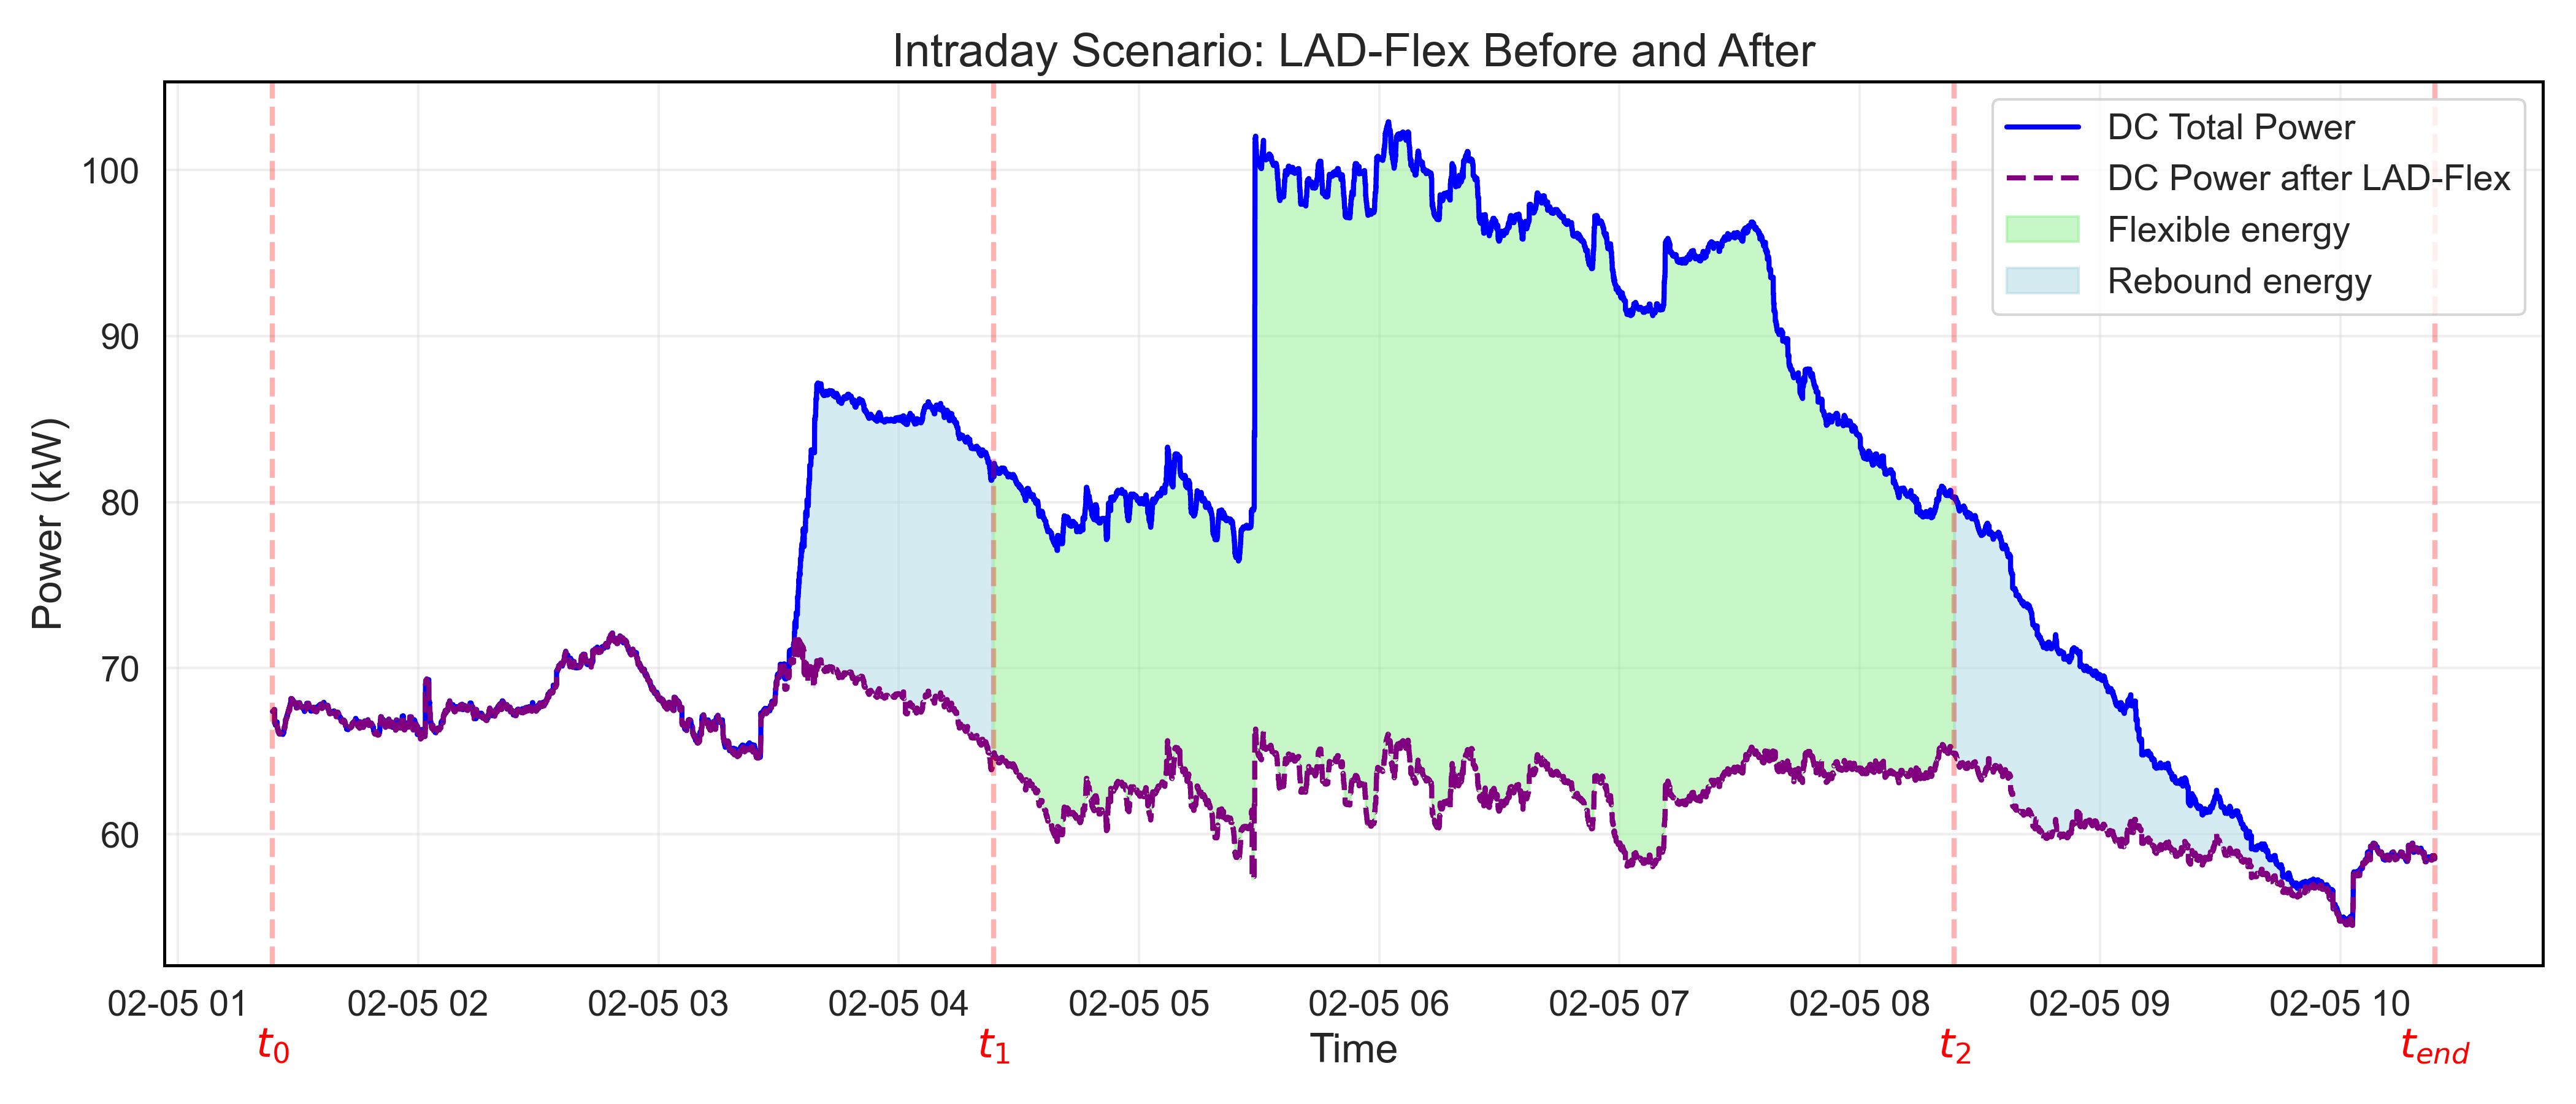
\includegraphics[width=14cm]{LAD_flex_P1_explanation_DEFAULT_DAM.png}
    \caption{Estimated GPU-side power of the modeled IT workload before and after LAD-Flex activation for point P1 under the Intraday scenario.}
    \label{fig:LAD_flex_summary_intraday}
\end{figure}

Table~\ref{tab:energy_flexibility_intraday} summarizes the key metrics for the selected points. The Intraday scenario achieves notably higher flexibility percentages compared to the baseline. Points P1–P3 demonstrate deferral percentages between 28\% and 33\%, with P2 achieving the highest percentage (33.11\%) despite having fewer tasks than P1. This suggests that the characteristics of individual tasks—particularly their duration and power consumption—play a significant role in determining flexibility potential beyond task count alone.

The total deferrable energy at peak points exceeds 100~kWh. Points Q1–Q3 show flexibility percentages around 3.3–3.7\%, while the median points R1–R3 achieve 1.2–1.8\% deferral. These lower-percentile values are comparable to the Baseline scenario, indicating that the extended parameters primarily benefit periods with high concentrations of deferrable workloads rather than uniformly increasing flexibility across all operating conditions.

\begin{table}[h!]
\centering
\renewcommand{\arraystretch}{1.2}
\begin{tabular}{@{}lrr rrr@{}}
\toprule
\textbf{Point} & \multicolumn{1}{c}{\textbf{Tasks}} & \multicolumn{3}{c}{\textbf{Energy}} \\
              & \textbf{Count} & \textbf{Deferrable (kWh)} & \textbf{Total (kWh)} & \textbf{Percentage Def. (\%)} \\
\midrule
P1 & 252 & 108.70 & 359.90 & 30.20 \\
P2 & 100 & 102.30 & 308.92 & 33.11 \\
P3 & 88  & 78.47  & 282.26 & 27.80 \\
Q1 & 8   & 9.26   & 276.44 & 3.35  \\
Q2 & 40  & 9.98   & 272.32 & 3.67  \\
Q3 & 15  & 8.89   & 251.39 & 3.54  \\
R1 & 32  & 3.01   & 166.49 & 1.81  \\
R2 & 23  & 2.90   & 243.12 & 1.19  \\
R3 & 19  & 2.88   & 179.20 & 1.61  \\
\bottomrule
\end{tabular}
\caption{Breakdown of task and energy flexibility by point for the Intraday scenario.}
\label{tab:energy_flexibility_intraday}
\end{table}


%%%%%%%%%%%%%%%%%%%%%%%%%%%%%%%%%%%%%%%%%%%%%%%%%%%%%%%%%%%%%%%%%%%%%%%%%%%%%%%
\subsubsection{mFRR Balancing Reserve Scenario} \label{mfrr_scenario}
%%%%%%%%%%%%%%%%%%%%%%%%%%%%%%%%%%%%%%%%%%%%%%%%%%%%%%%%%%%%%%%%%%%%%%%%%%%%%%%

The mFRR scenario represents the most demanding market configuration modelled in terms of response time requirements. mFRR markets require rapid activation with minimal advance notice to address frequency deviations and power imbalances, testing the limits of LAD-Flex's real-time responsiveness. Table~\ref{tab:parameters_mfrr} presents the LAD-Flex parameters configured for this scenario.

\begin{table}[h!]
\centering
\begin{tabular}{@{}cccccc@{}}
\toprule
\textbf{Scenario} & $\hat{\lambda}$ & $\beta_\text{overhang}$ & $\gamma_{\text{buffer}}$ & $\delta_{\text{notification}}$ & $\eta{\Delta t}$ \\ \midrule
mFRR & 3 min & 0.8 & 20 min & 15 min & 1 h \\ \bottomrule
\end{tabular}
\caption{LAD-Flex parameters for the mFRR balancing reserve scenario.}
\label{tab:parameters_mfrr}
\end{table}

The mFRR scenario is characterized by a short flexibility window ($\eta{\Delta t} = 1$~h), a brief notification period ($\delta_{\text{notification}} = 15$~min), and a reduced latency threshold ($\hat{\lambda} = 3$~min). The lower latency threshold increases the pool of tasks eligible for deferral, compensating for the limited time available to accumulate flexible workload. The overhang parameter ($\beta_{\text{overhang}} = 0.8$) allows tasks that nearly fit within the 1-hour window to still qualify, while the reduced buffer period ($\gamma_{\text{buffer}} = 20$~min) reflects the tighter timing constraints of balancing markets.

Fig.~\ref{fig:LAD_flex_points_mfrr} shows the deferrable energy for each hourly activation throughout the sample week. The mFRR scenario yields considerably lower volumes of flexible energy per activation compared to the baseline and Intraday scenarios, with peak deferrable energy reaching approximately 7~kWh. This reduction is expected given the shorter flexibility window and the limited time for task accumulation during the brief notification period. Nevertheless, the strategy identifies consistent flexibility potential across the week, with several periods offering meaningful deferral capacity for grid balancing purposes.

\begin{figure}[!h]
    \centering
    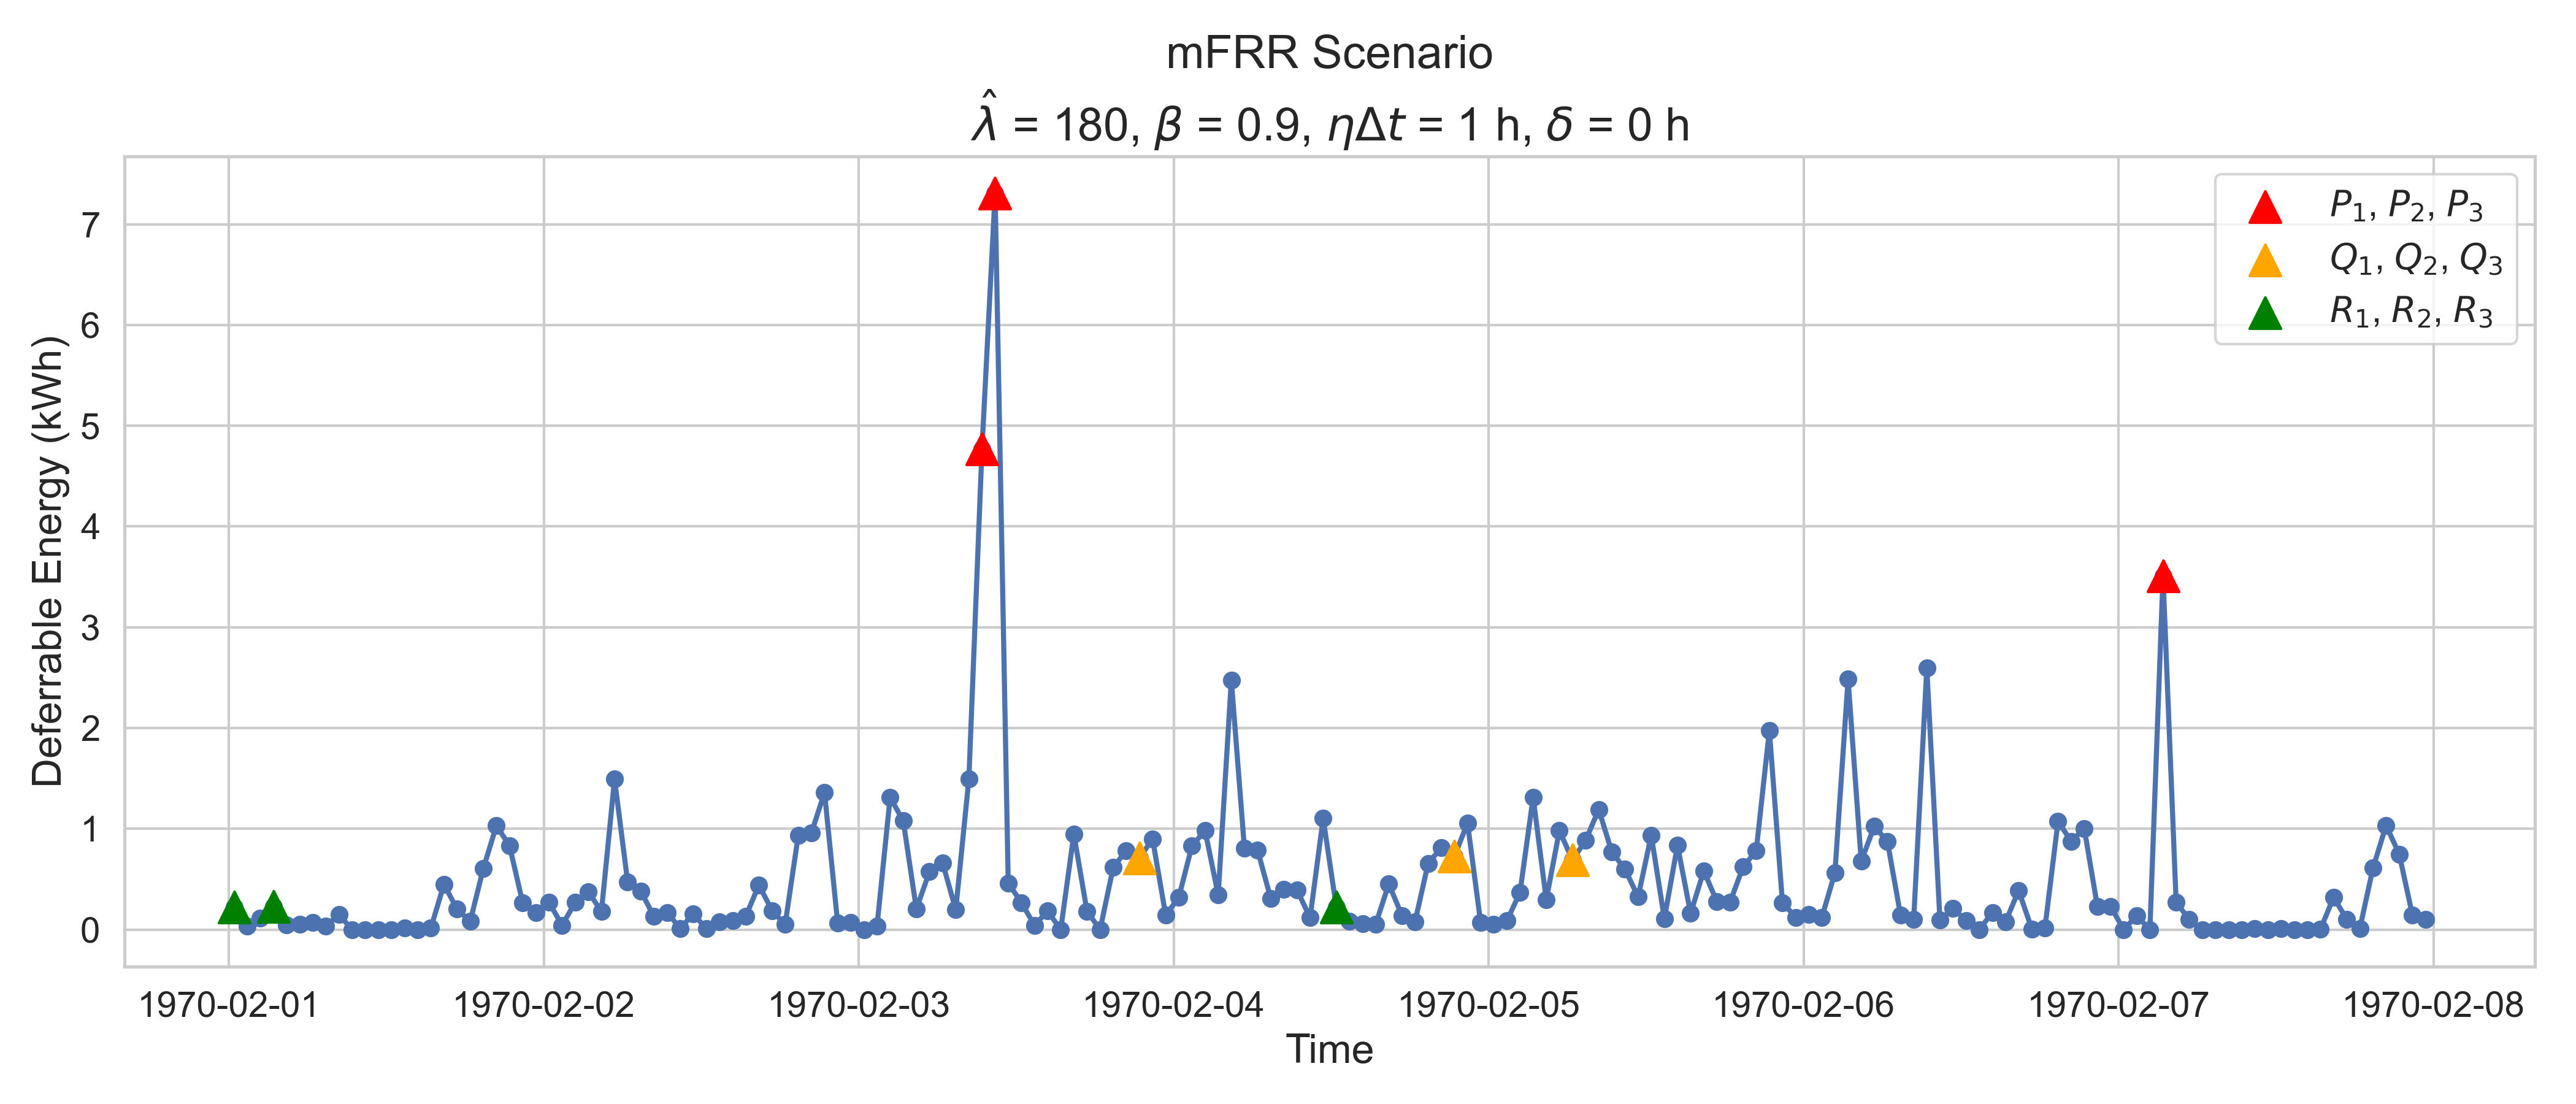
\includegraphics[width=14cm]{LARGE_DEFAULT_mFRR_ZETA_0.png}
    \caption{Deferred energy from LAD-Flex executed hourly over the sample week for the mFRR scenario.}
    \label{fig:LAD_flex_points_mfrr}
\end{figure}

Fig.~\ref{fig:LAD_flex_points_grid_mfrr} illustrates the deferred power profiles for the nine selected points. At high-flexibility instances (P1–P3), deferred power exhibits rapid ramp-up behavior, with P1 reaching nearly 20~kW and P2 exceeding 15~kW. These steep profiles align well with mFRR activations, where substantial power must be shifted within a narrow time window.

The short notification period (15~min, shown in green) provides limited time for task accumulation before the flexibility window begins. For the mid-range points (Q1–Q3), deferred power peaks around 0.8–1.2~kW, while the median points (R1–R3) show values in the range of 0.2–1.0~kW. Despite these lower magnitudes, the strategy demonstrates its ability to respond to short-notice flexibility requests consistently.

\begin{figure}[!h]
    \centering
    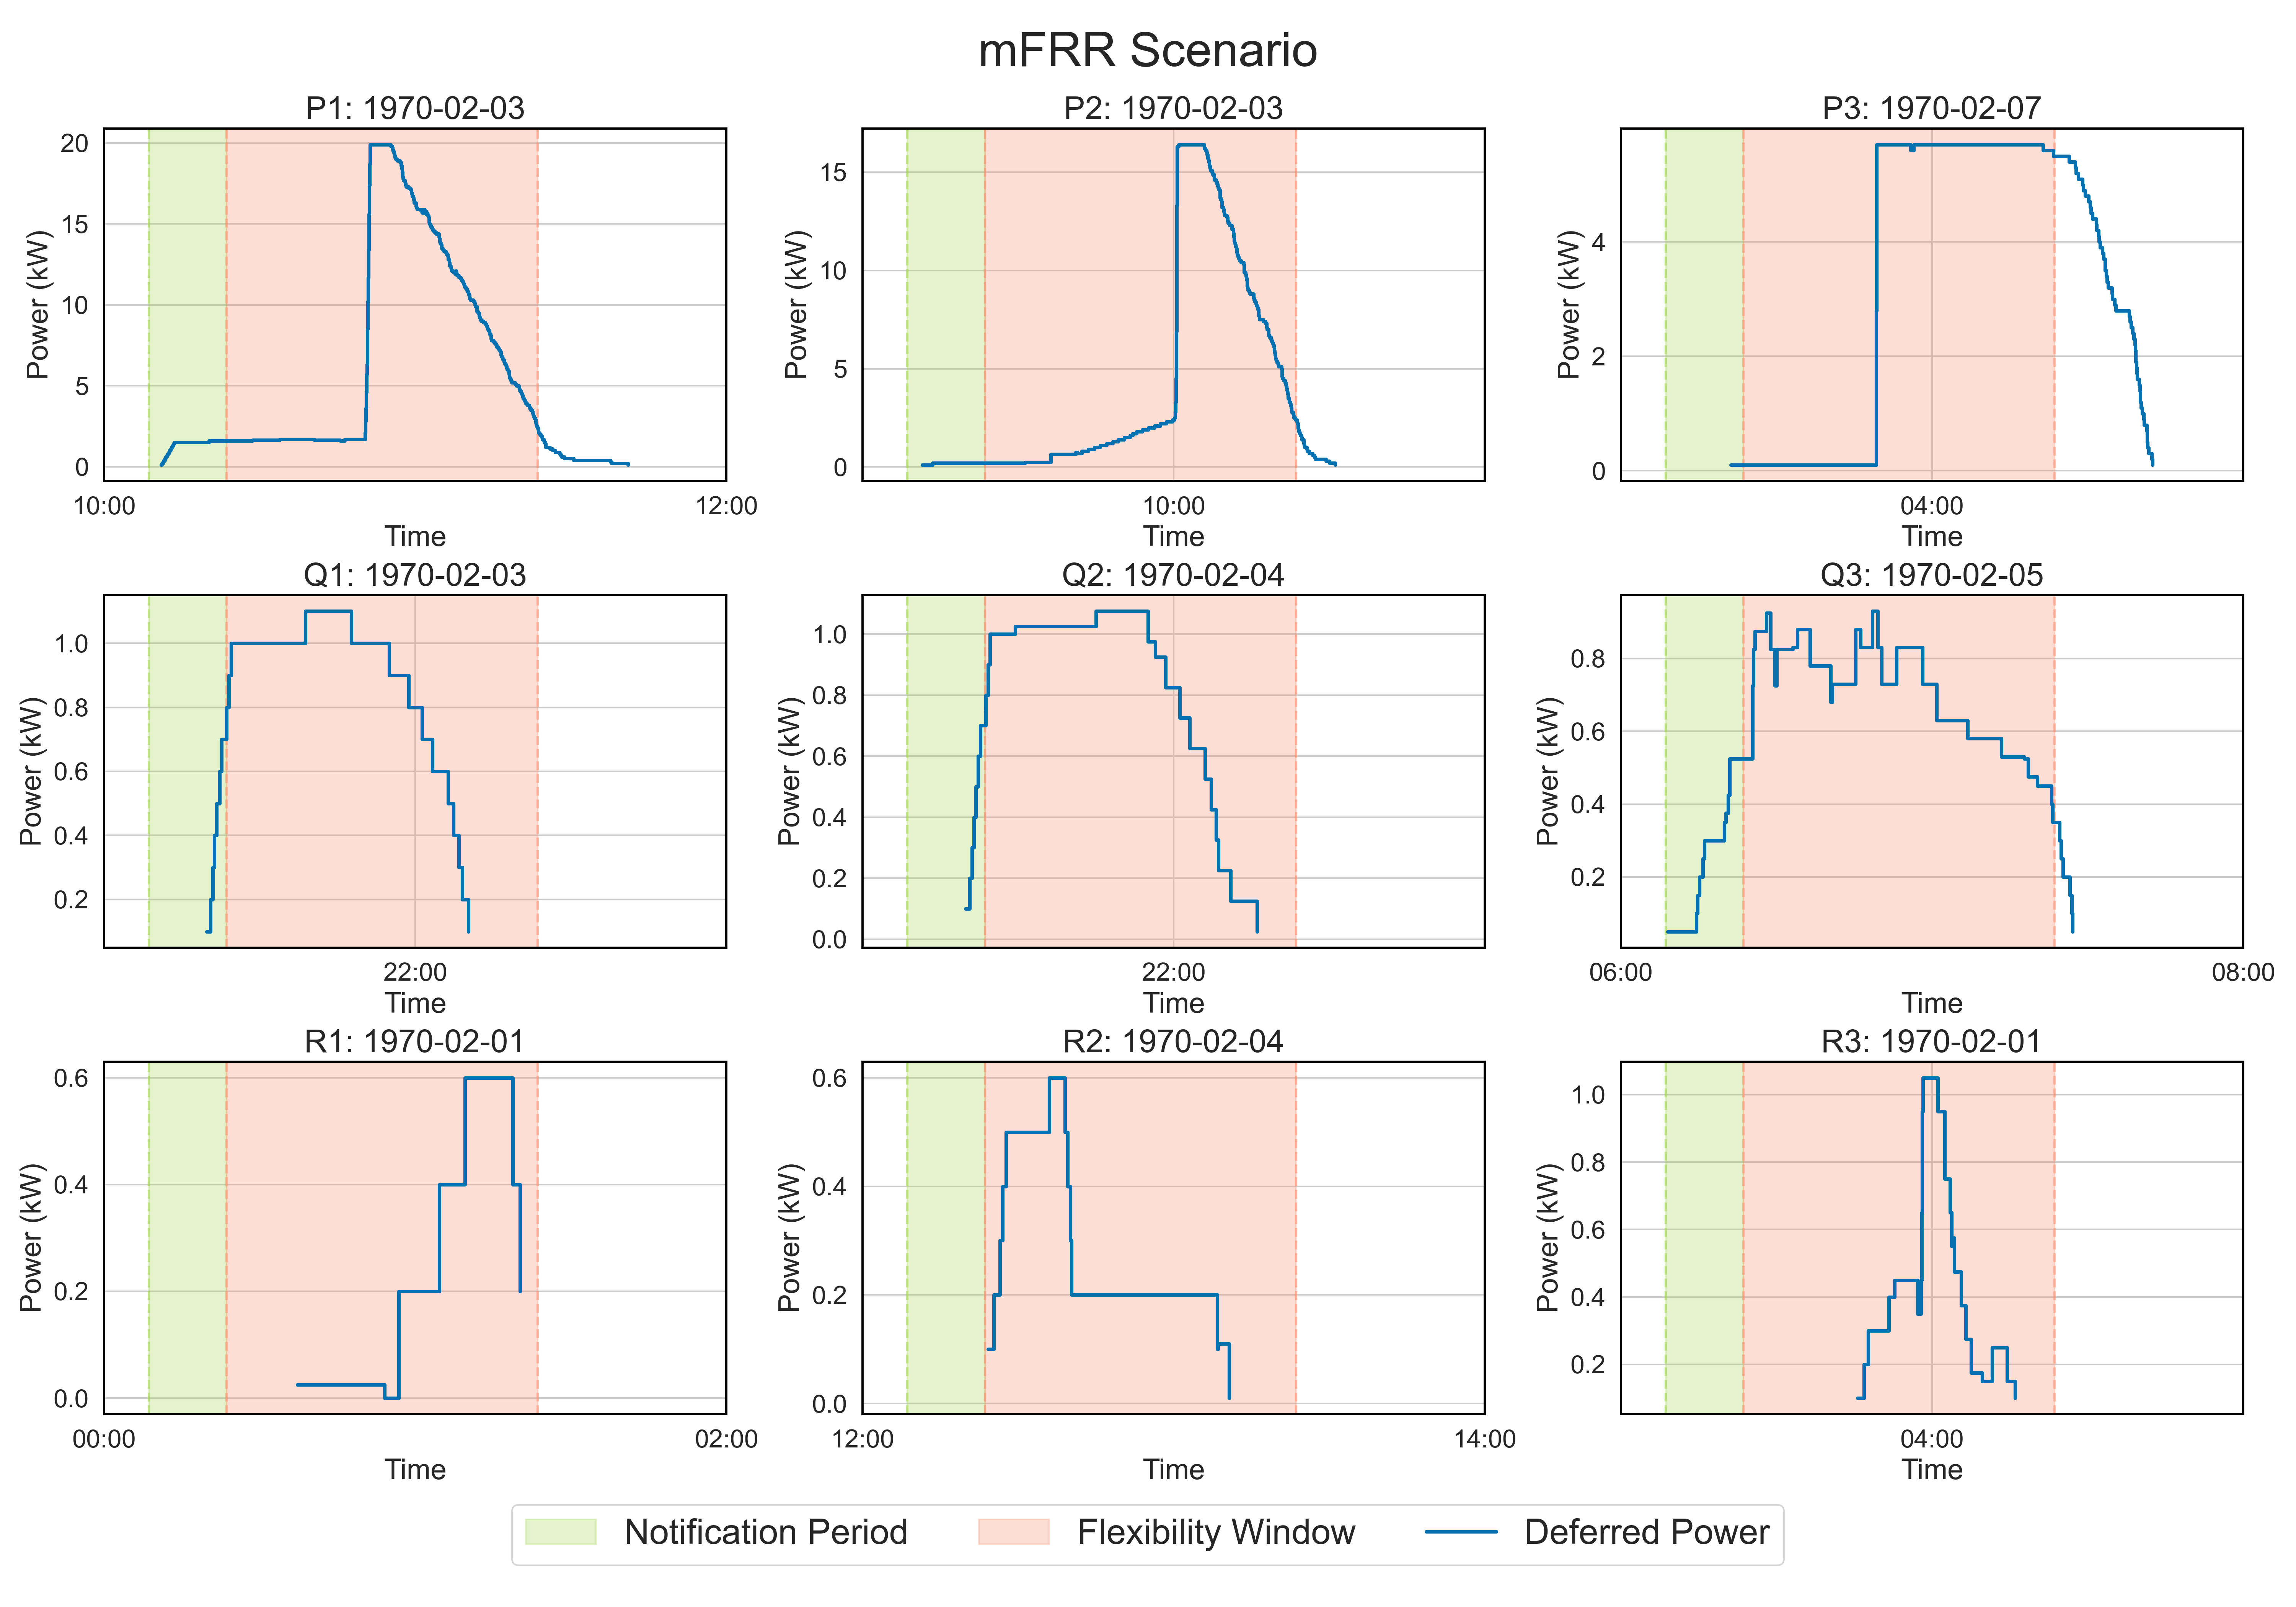
\includegraphics[width=14cm]{power_consumption_3x3_LARGE_DEFAULT_mFRR.png}
    \caption{Deferred power profiles for LAD-Flex activations under the mFRR scenario for the 9 selected instants.}
    \label{fig:LAD_flex_points_grid_mfrr}
\end{figure}

Fig.~\ref{fig:LAD_flex_summary_mfrr} presents the estimated GPU-side power of the modeled IT workload before and after LAD-Flex activation at point P1. The original IT-side power demand (blue) shows a significant spike reaching approximately 90~kW during the flexibility window. After applying LAD-Flex, the adjusted consumption (purple dashed line) remains stable around 50–55~kW, effectively shaving the peak demand. Notably, the rebound energy in this scenario is minimal due to the short notification period and compact flexibility window.

\begin{figure}[!h]
    \centering
    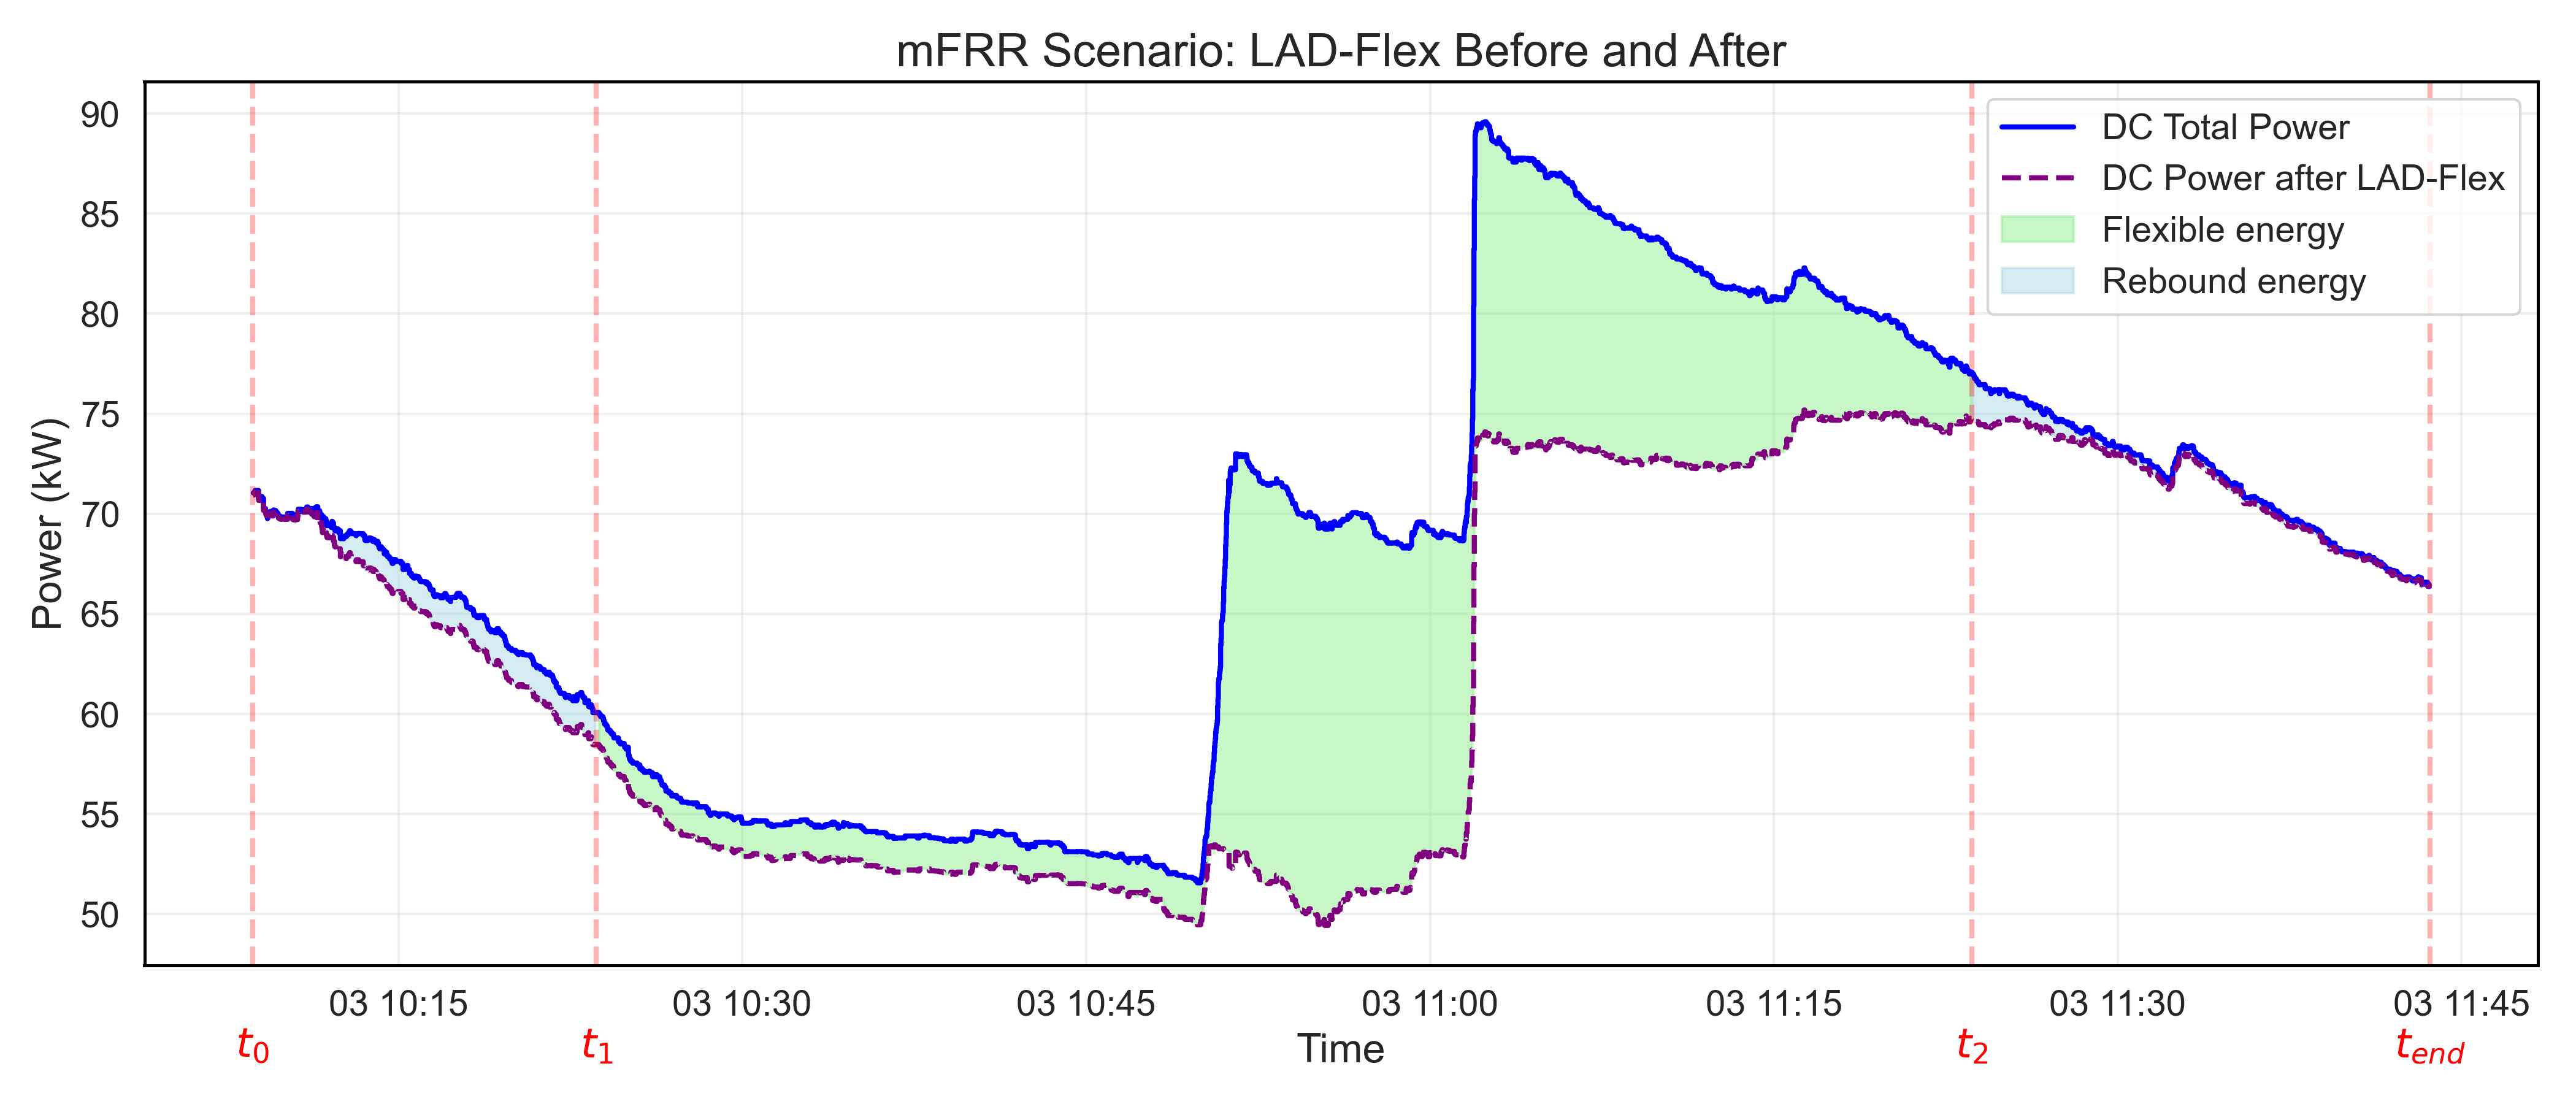
\includegraphics[width=14cm]{LAD_flex_P1_explanation_DEFAULT_mFRR.png}
    \caption{Estimated GPU-side power of the modeled IT workload before and after LAD-Flex activation for point P1 under the mFRR scenario.}
    \label{fig:LAD_flex_summary_mfrr}
\end{figure}

Table~\ref{tab:energy_flexibility_mfrr} summarizes the key metrics for the selected points. While the absolute deferrable energy values are lower than in other scenarios, the flexibility percentages at peak points remain notable: P1 achieves 10.84\% deferral, with P2 and P3 reaching 7.01\% and 5.11\% respectively. These percentages demonstrate that even under stringent mFRR requirements, LAD-Flex can identify and defer a meaningful fraction of the DC's workload.

The task counts at peak points (P1: 208 tasks, P2: 162 tasks) indicate that the strategy successfully filters a large number of short-duration tasks that meet the strict latency and overhang criteria. The lower latency threshold ($\hat{\lambda} = 3$~min) enables a broader pool of tasks to be considered, partially compensating for the shorter activation window. Points Q1–Q3 show flexibility percentages between 0.7\% and 1.6\%, while median points R1–R3 achieve 0.3–0.5\% deferral. These lower-percentile values reflect the challenge of finding suitable tasks under mFRR's demanding constraints, yet still represent actionable flexibility for grid balancing purposes.

\begin{table}[h!]
\centering
\renewcommand{\arraystretch}{1.2}
\begin{tabular}{@{}lrr rrr@{}}
\toprule
\textbf{Point} & \multicolumn{1}{c}{\textbf{Tasks}} & \multicolumn{3}{c}{\textbf{Energy}} \\
              & \textbf{Count} & \textbf{Deferrable (kWh)} & \textbf{Total (kWh)} & \textbf{Percentage Def. (\%)} \\
\midrule
P1 & 208 & 7.31  & 67.43  & 10.84 \\
P2 & 162 & 4.77  & 68.02  & 7.01  \\
P3 & 58  & 3.51  & 68.75  & 5.11  \\
Q1 & 11  & 0.71  & 44.41  & 1.60  \\
Q2 & 12  & 0.73  & 57.73  & 1.26  \\
Q3 & 23  & 0.69  & 95.37  & 0.72  \\
R1 & 4   & 0.23  & 48.97  & 0.46  \\
R2 & 7   & 0.22  & 67.25  & 0.33  \\
R3 & 14  & 0.23  & 57.53  & 0.40  \\
\bottomrule
\end{tabular}
\caption{Breakdown of task and energy flexibility by point for the mFRR scenario.}
\label{tab:energy_flexibility_mfrr}
\end{table}

The mFRR results demonstrate that DCs can participate in high-value balancing markets where responsiveness commands premium compensation, despite potentially lower flexibility volumes compared to longer-notice products. The trade-off between response time and flexibility volume is further explored in Section~\ref{sec:scenario_comparison}.







%%%%%%%%%%%%%%%%%%%%%%%%%%%%%%%%%%%%%%%%%%%%%%%%%%%%%%%%%%%%%%%%%%%%%%%%%%%%%%%
\subsubsection{Scenario Comparison} \label{sec:scenario_comparison}
%%%%%%%%%%%%%%%%%%%%%%%%%%%%%%%%%%%%%%%%%%%%%%%%%%%%%%%%%%%%%%%%%%%%%%%%%%%%%%%

A comparative analysis of LAD-Flex performance across the three market scenarios is necessary, to highlight the trade-offs between flexibility volume, response time requirements, and operational efficiency.

Firstly, Fig.~\ref{fig:time_series_comparison} presents a time series overlay of deferrable energy, flexibility percentage, and task count across all three scenarios throughout the sample week. As mentioned before, these plots reveal that flexibility potential is highly variable and strongly correlated with workload characteristics. All three scenarios exhibit pronounced spikes during certain periods, indicating that the availability of deferrable tasks is not uniformly distributed but rather concentrated in specific time intervals. The Intraday scenario consistently achieves the highest peaks in deferrable energy. The Baseline scenario follows a similar temporal pattern but with lower peak magnitudes. Of the three, the mFRR scenario shows substantially lower values throughout the week, reflecting the constraints imposed by its shorter flexibility window and notification period.

Notably, the timing of peak flexibility events is mostly consistent across scenarios, suggesting that the underlying workload composition—rather than the scenario-specific parameters—drives the temporal distribution of flexibility potential. This observation has practical implications for aggregators: coordinating flexibility requests with periods of high non-critical workload concentration can significantly enhance the value extracted from DC participation in DR programs.

\begin{figure}[!h]
    \centering
    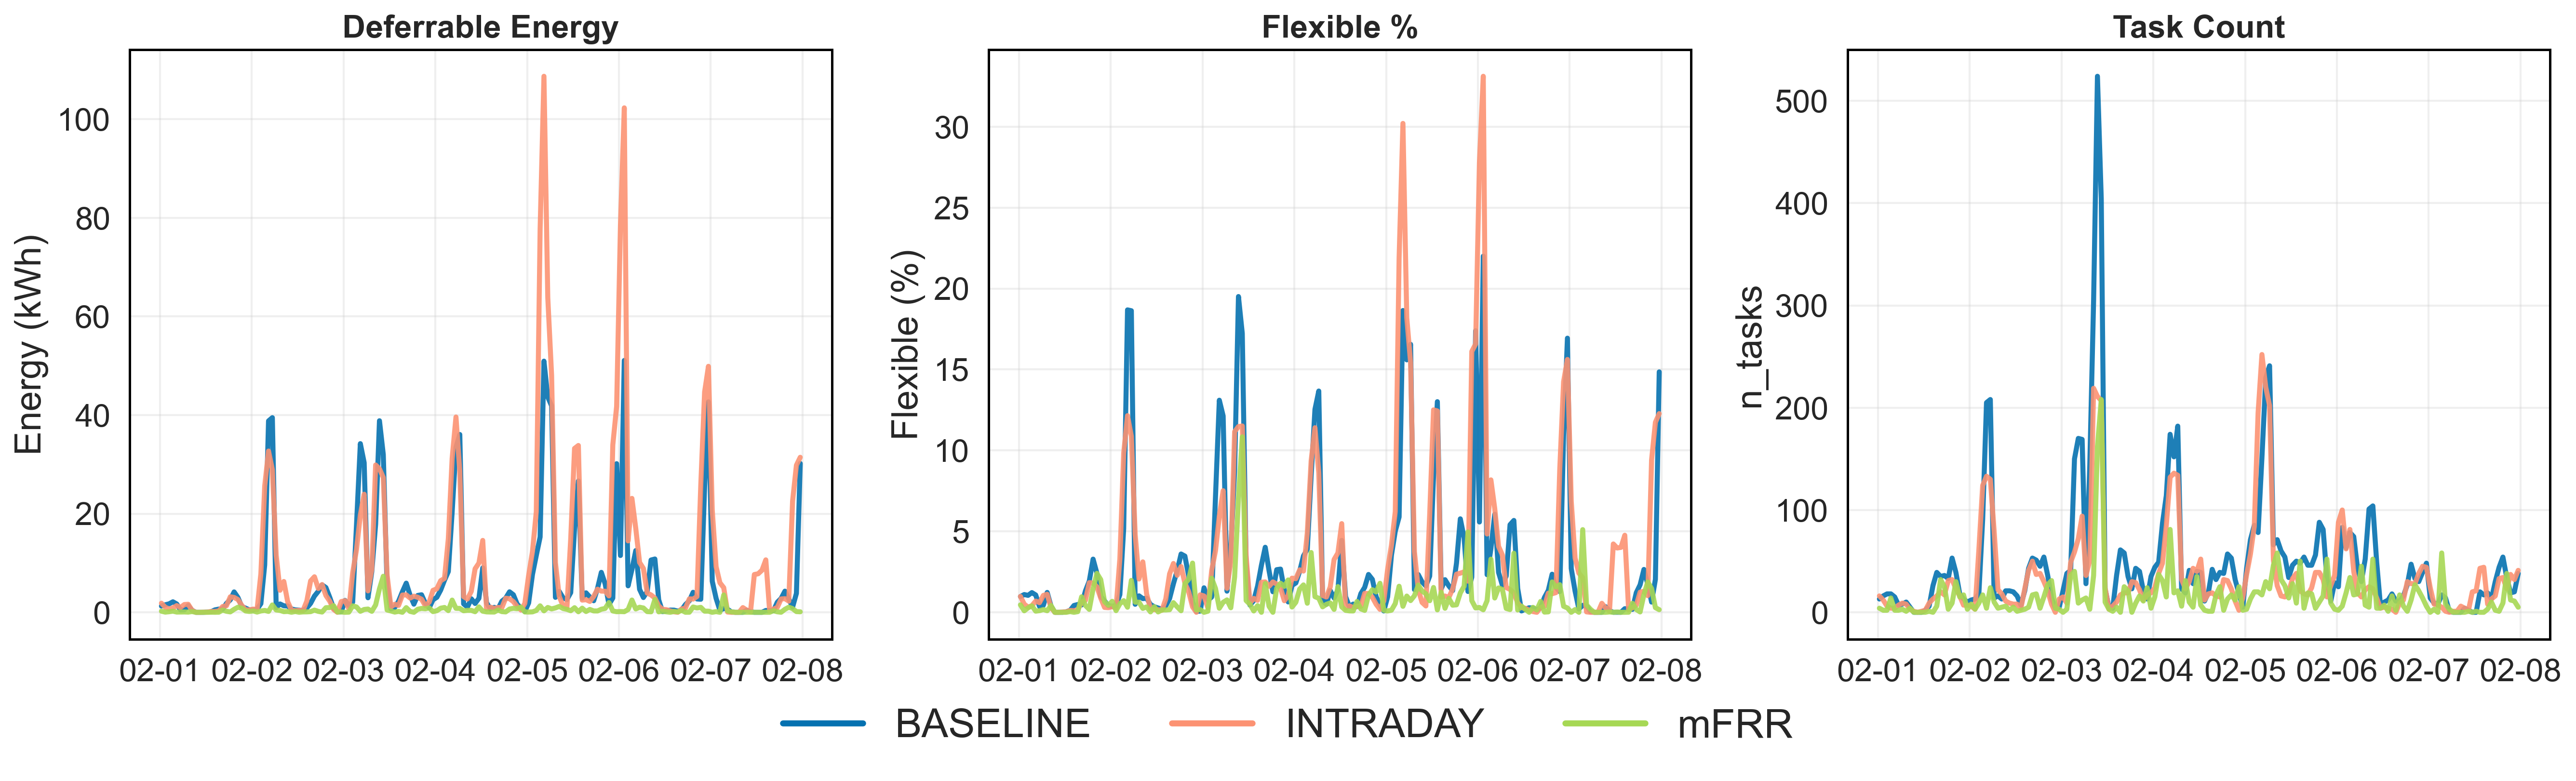
\includegraphics[width=\textwidth]{time_series_overlay_sample_week.png}
    \caption{Time series comparison of deferrable energy, flexibility percentage, and task count across the three market scenarios over the sample week.}
    \label{fig:time_series_comparison}
\end{figure}

Further analysing the statistical distribution of flexibility metrics, Fig.~\ref{fig:boxplot_comparison} presents box plots comparing the distribution of deferrable energy, flexibility percentage, and task count across the three scenarios. In terms of deferrable energy, the Intraday scenario exhibits the highest median and the widest interquartile range, reflecting both greater average flexibility and higher variability. The Baseline scenario shows a more compact distribution with a lower median, while the mFRR scenario is characterized by a narrow distribution concentrated near zero, with limited variability.

The flexibility percentage distributions reveal an interesting pattern: while the Intraday scenario achieves the highest absolute energy values, the Baseline scenario shows competitive flexibility percentages during peak events. This suggests that the baseline configuration, with its moderate parameters, can efficiently capture available flexibility relative to total DC consumption during favorable periods.

The task count distributions indicate that the Baseline scenario typically involves more tasks per activation than the Intraday scenario, despite achieving lower total deferrable energy. This is explained by the different latency thresholds: the baseline's lower threshold ($\hat{\lambda} = 10$~min) captures a larger number of shorter tasks, while the intraday's higher threshold ($\hat{\lambda} = 30$~min) filters for fewer but longer-duration tasks that contribute more energy per task.

\begin{figure}[!h]
    \centering
    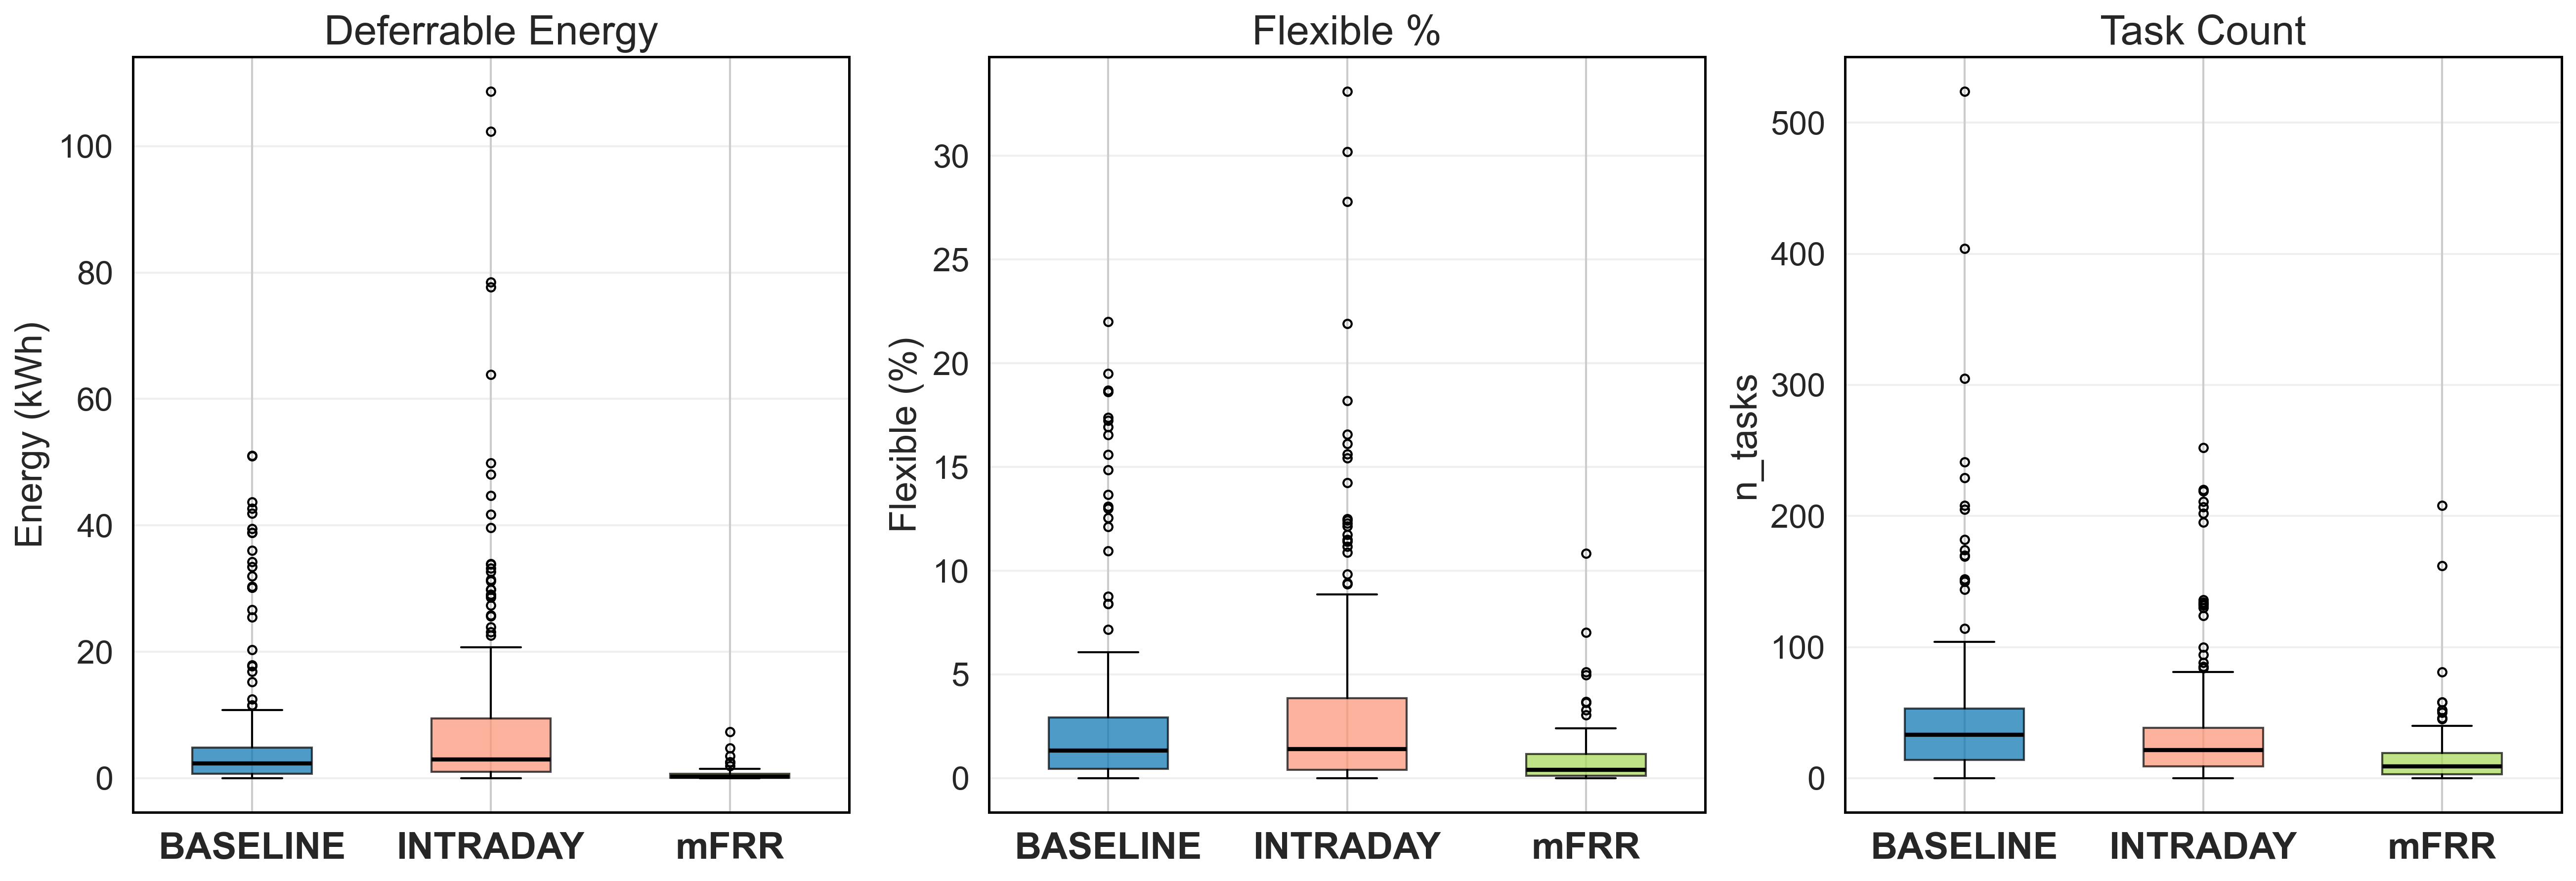
\includegraphics[width=\textwidth]{combined_comparison_publication_ready.png}
    \caption{Box plot comparison of deferrable energy, flexibility percentage, and task count distributions across the three market scenarios.}
    \label{fig:boxplot_comparison}
\end{figure}

Fig.~\ref{fig:notable_points_comparison} compares the deferrable energy at the nine representative points (P1-P3, Q1-Q3, R1-R3) across all three scenarios. This visualization synthesizes the findings from the individual scenario analyses and highlights the magnitude of differences between market configurations.

At peak flexibility points (P1-P3), the Intraday scenario delivers approximately twice the deferrable energy of the Baseline scenario, with values exceeding 100~kWh compared to approximately 50~kWh. The mFRR scenario, constrained by its 1-hour flexibility window, achieves only 3.5-7.3~kWh at these same point. This difference underscores the fundamental trade-off between response time and flexibility volume.

At mid-range points (Q1-Q3), representing the 75th percentile of flexibility potential, the gap between scenarios narrows in relative terms but remains substantial in absolute values. At median points (R1-R3), all scenarios converge toward lower values, with the baseline and intraday achieving similar performance (2.3-3.0~kWh) and mFRR remaining at approximately 0.2~kWh.

\begin{figure}[!h]
    \centering
    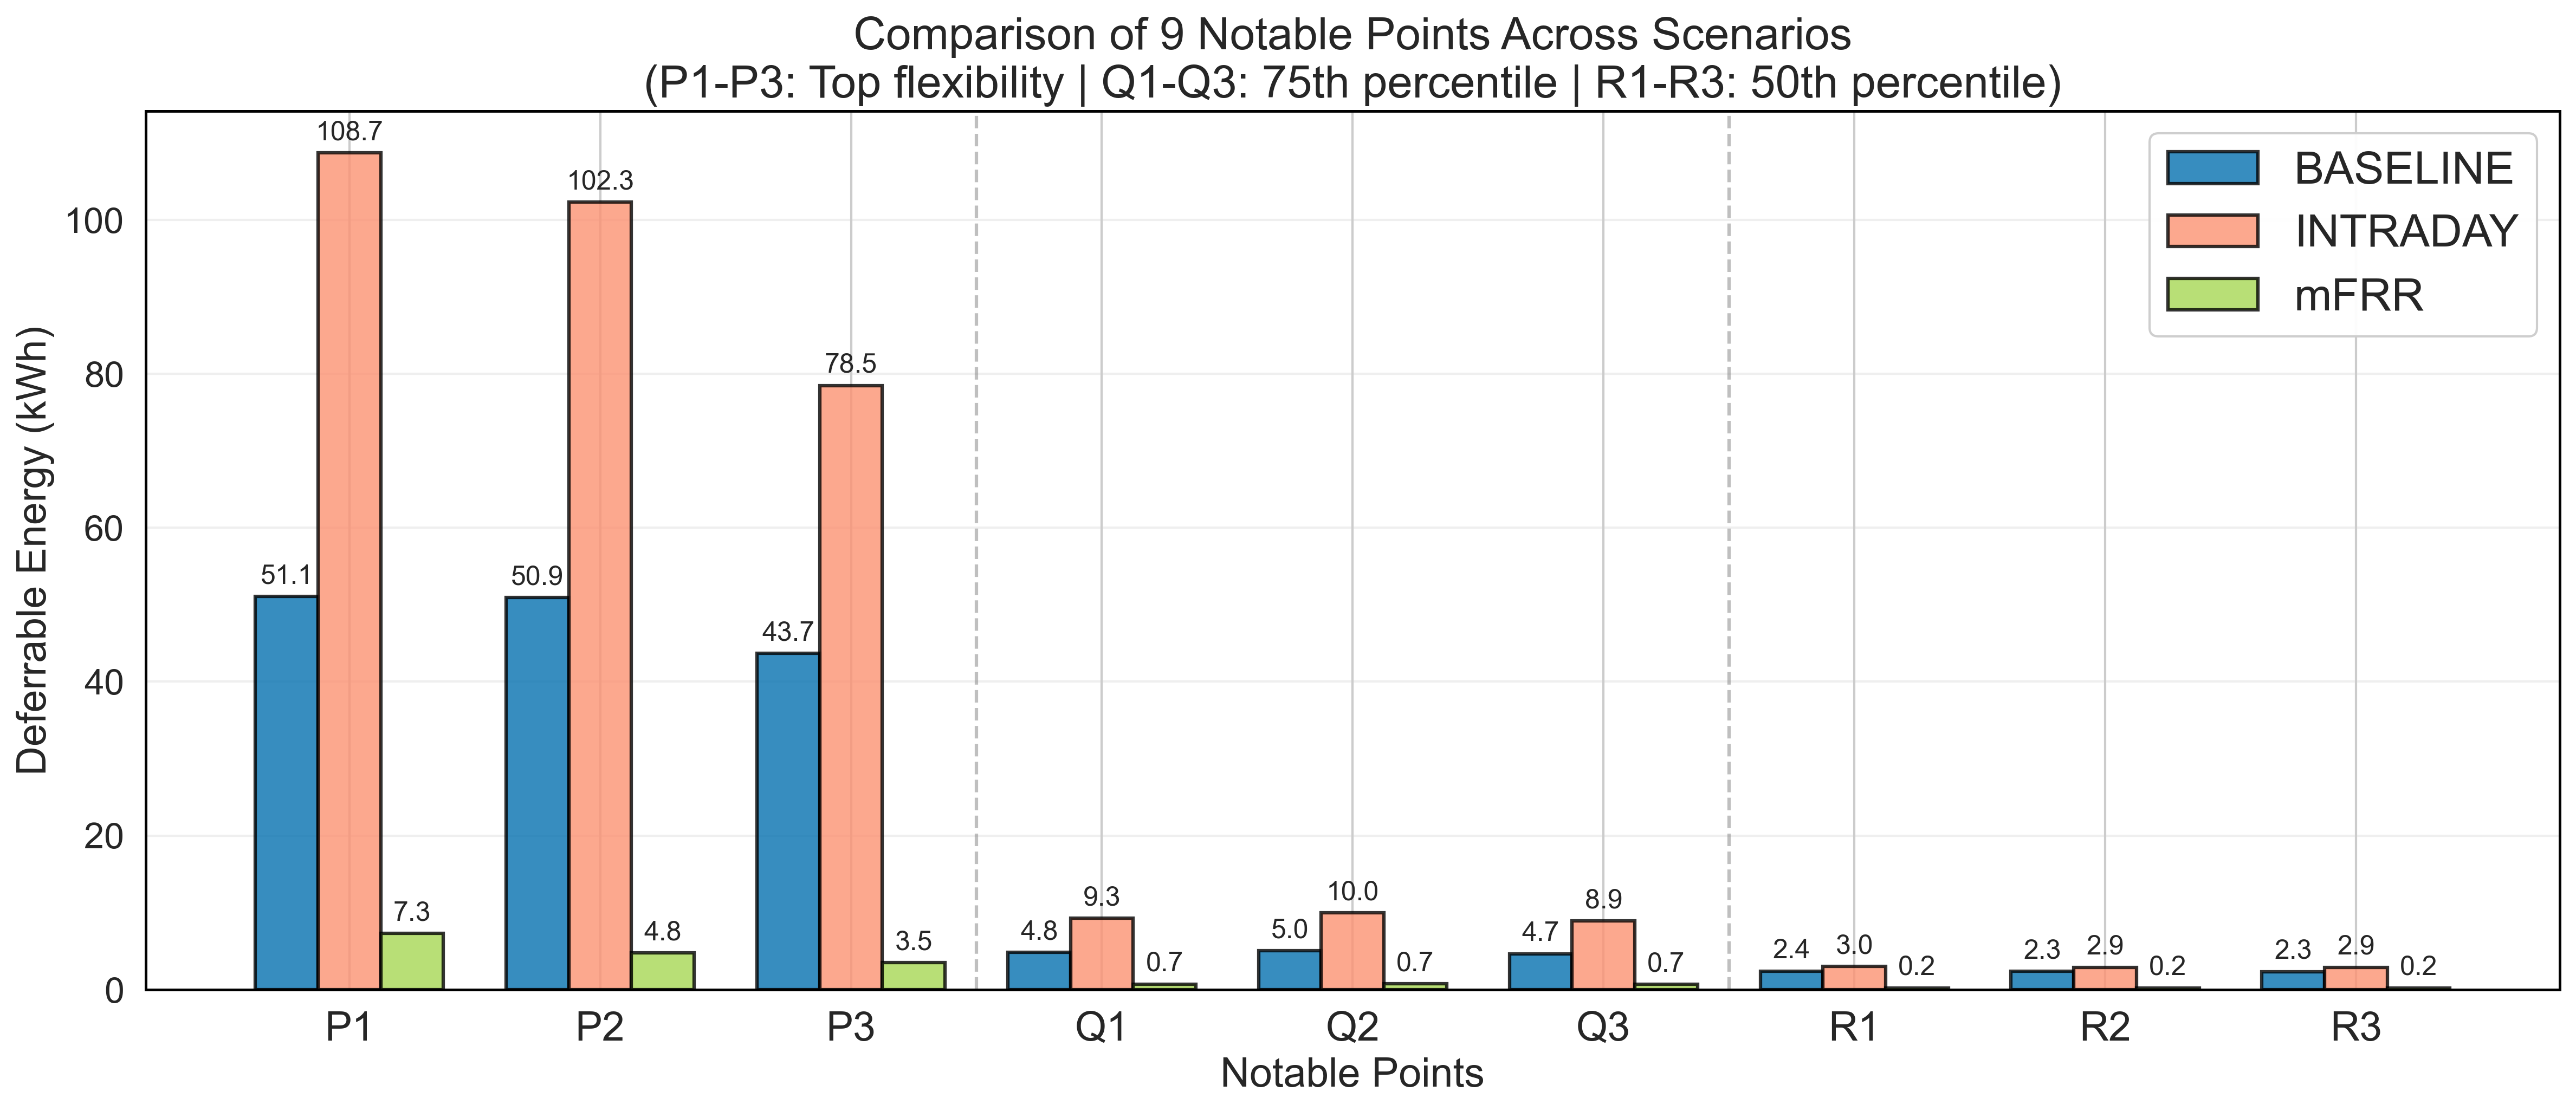
\includegraphics[width=\textwidth]{notable_points_comparison.png}
    \caption{Comparison of deferrable energy at the nine representative points across the three market scenarios.}
    \label{fig:notable_points_comparison}
\end{figure}

Finally, to enable a fair comparison across scenarios with different flexibility window durations, a new metric is introduced. The hourly flexibility yield $\theta$ is defined as the average deferrable energy per hour of flexibility window, computed across all hourly activations in the sample week:

\begin{equation}
    \theta = \frac{1}{168} \sum_{h=1}^{168} \frac{E_h^{\text{def}}}{\eta \Delta T}
    \label{eq:hourly_yield}
\end{equation}

\noindent where 168 is the number of hours in the sample week and $E_h^{\text{def}}$ is the deferrable energy when a flexibility window begins at hour $h$.

Fig.~\ref{fig:hourly_yield} presents the hourly flexibility yield for each scenario. The Intraday scenario achieves the highest yield at 2.51~kWh/h, followed closely by the baseline at 2.17~kWh/h. The mFRR scenario exhibits a lower yield of 0.50~kWh/h.

This metric reveals that the Intraday scenario not only delivers more total energy but also extracts flexibility more efficiently per unit time of the flexibility window. The Baseline scenario, despite its shorter 3-hour window compared to the intraday's 4-hour window, achieves comparable yield, suggesting that the additional hour in the Intraday scenario provides diminishing returns in terms of energy capture rate.

The low yield of the mFRR scenario reflects the fundamental challenge of providing balancing reserves through workload deferral: the short notification period (15~min) limits the strategy's ability to accumulate deferrable tasks before the flexibility window begins. However, this lower yield must be weighed against the higher market value typically associated with fast-response flexibility products.

\begin{figure}[!h]
    \centering
    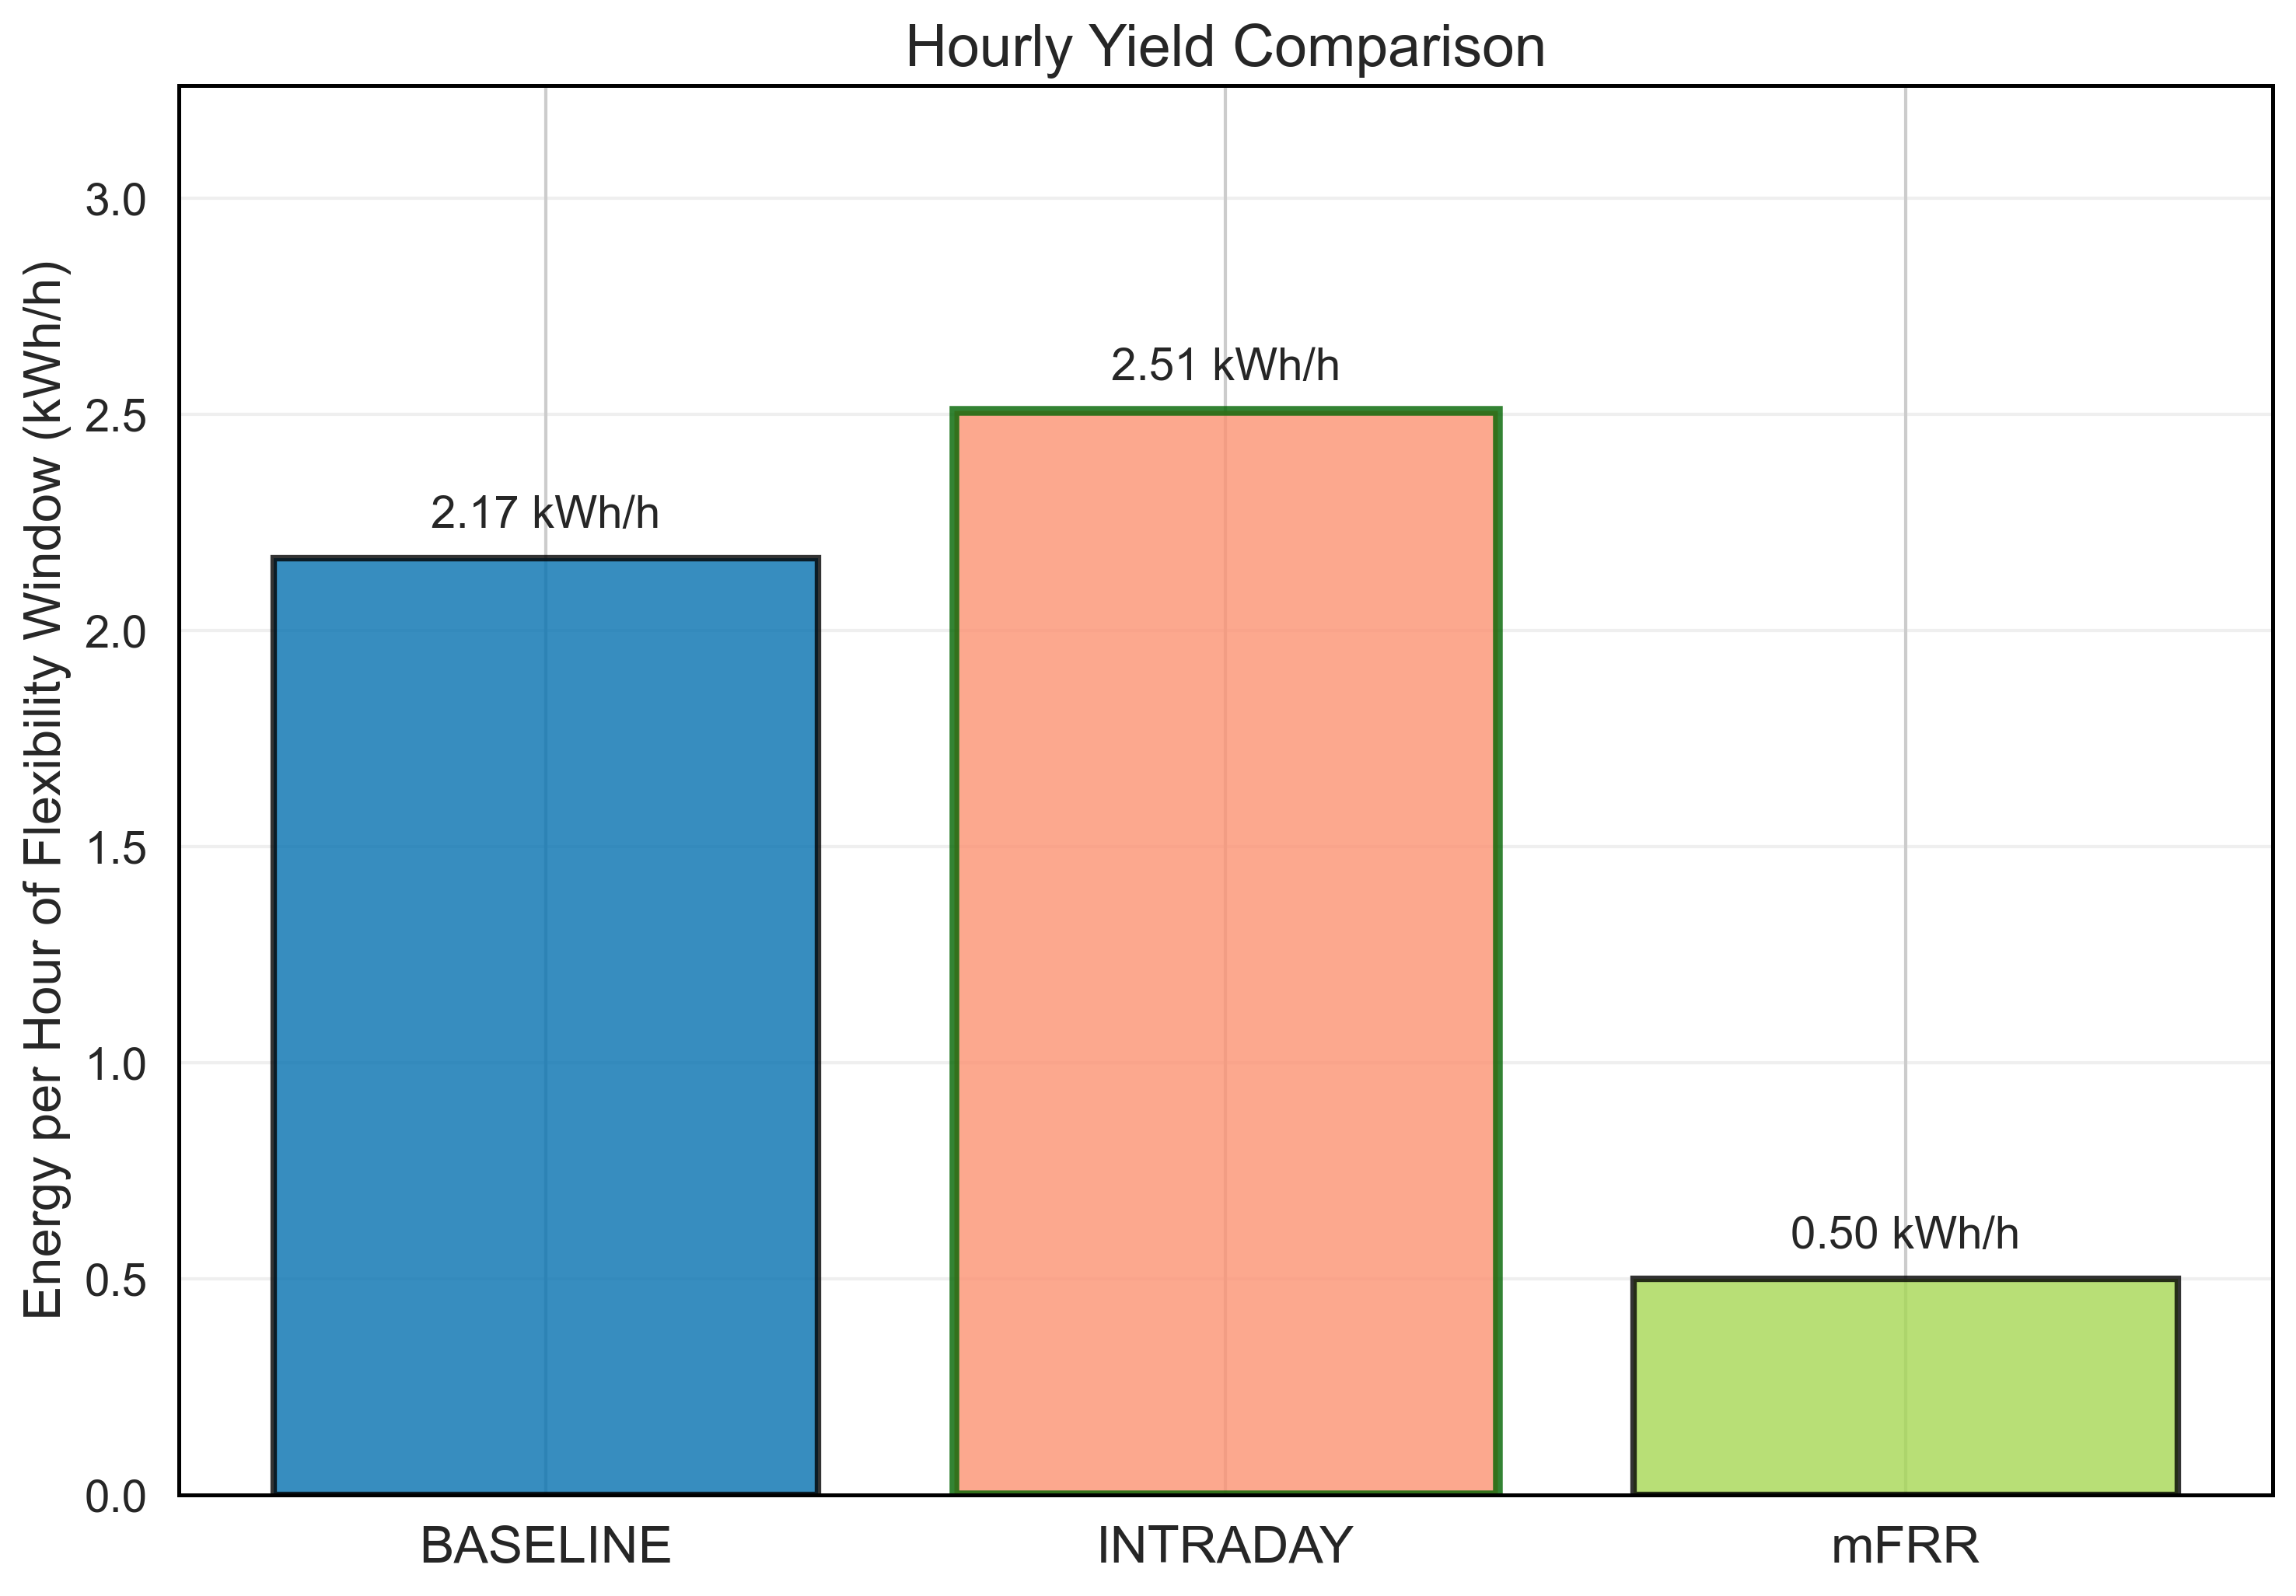
\includegraphics[width=0.8\textwidth]{hourly_yield_comparison.png}
    \caption{Hourly flexibility yield comparison across the three market scenarios, measuring average deferrable energy per hour of flexibility window.}
    \label{fig:hourly_yield}
\end{figure}

While the hourly flexibility yield quantifies the rate of energy capture per unit time of the flexibility window, it does not characterize the extent to which the energy impact of deferral is contained within the contracted flexibility period. In any LAD-Flex activation, two distinct forms of rebound may arise, and it is important to distinguish between them.

The first is activation-window spillover: energy from tasks classified as deferrable that is consumed outside the flexibility window $[t_1, t_2]$ but is still part of the same activation event. This spillover has two sources. During the notification period preceding $t_1$, tasks begin transitioning into deferral, and some task energy is consumed before the window opens. Similarly, during the buffer period following $t_2$, tasks permitted by the overhang parameter $\beta$ may finish executing beyond the window boundary. The rebound energy $E_{\text{rebound}}$ reported in this study captures precisely this spillover component.

The second form is rescheduling rebound: the deferred tasks must eventually execute, consuming the same energy at a later time. Unlike classical demand-response rebound in thermal systems, where deferred cooling or heating creates a compensatory surge driven by physical dynamics, workload deferral involves no such physical penalty. The deferred tasks consume identical energy regardless of when they are executed, and the DC operator retains full discretion over when to reschedule them, subject only to the constraint of avoiding overlap with future flexibility activations. The rescheduling of deferred workloads is therefore a DC-internal scheduling optimization problem, separate from the flexibility assessment framework presented here, and is not quantified in this analysis.

To quantify activation-window spillover, the Rebound Ratio ($RR$) is defined as the fraction of total activation-related energy that falls outside the flexibility window:

\begin{equation}
    RR = \frac{E_{\text{rebound}}}{E_{\text{def}} + E_{\text{rebound}}}
    \label{eq:rebound_ratio}
\end{equation}

\noindent where $E_{\text{def}}$ is the deferrable energy within $[t_1, t_2]$ and $E_{\text{rebound}}$ is the energy consumed in the notification and buffer periods $[t_0, t_1) \cup (t_2, t_{\text{end}}]$. Low values of $RR$ indicate that the flexibility delivery is well contained within the contracted window, with minimal energy spillover.

Fig.~\ref{fig:rebound_ratio} presents the Rebound Ratio across the three scenarios over the sample week. The Baseline scenario exhibits the highest mean $RR$ of 0.044, reflecting its longer notification period (60~min) and wider overhang tolerance ($\beta = 0.7$), which allow more task energy to spill outside the flexibility window boundaries. The Intraday scenario achieves an intermediate value of 0.029, while the mFRR scenario yields the lowest mean $RR$ of 0.014, consistent with its stringent timing constraints (15~min notification, $\beta = 0.9$) that restrict eligibility to tasks whose execution fits tightly within the activation window. Across all three scenarios, the Rebound Ratio remains between 1.4\% and 4.4\%, confirming that activation-window spillover is limited and that the vast majority of the energy impact of LAD-Flex is contained within the contracted flexibility period.

\begin{figure}[!h]
    \centering
    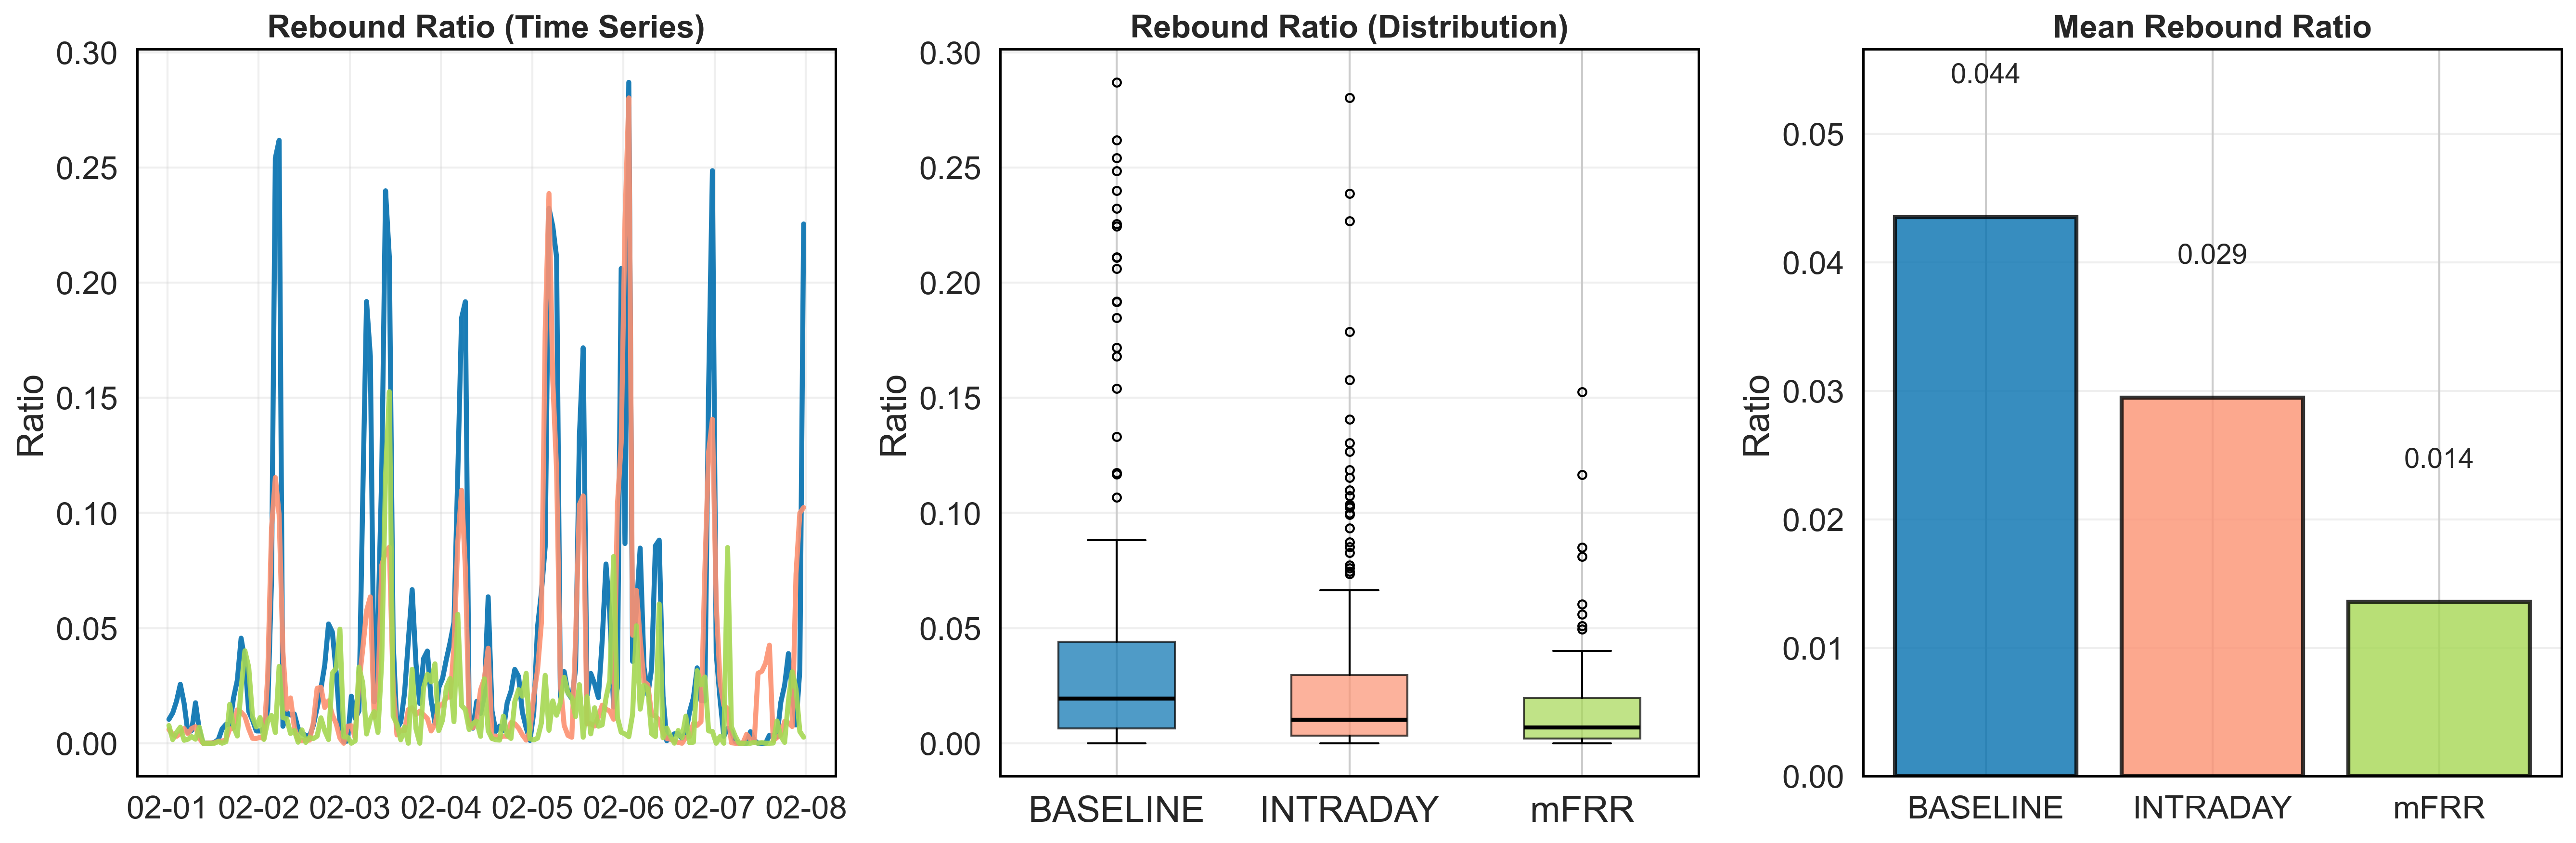
\includegraphics[width=\textwidth]{rebound_energy_summary.png}
    \caption{Rebound Ratio across the three market scenarios: time series over the sample week (left), distribution (center), and mean values (right). The Rebound Ratio measures the fraction of activation-related energy that falls outside the flexibility window.}
    \label{fig:rebound_ratio}
\end{figure}

Concluding the comparison of the scenarios, Table~\ref{tab:scenario_summary} summarizes the key performance indicators across the three scenarios. The results demonstrate that DCs can participate in multiple electricity market products through latency-aware workload deferral, with the choice of market depending on operational priorities and revenue optimization strategies.

\begin{table}[h!]
\centering
\renewcommand{\arraystretch}{1.2}
\begin{tabular}{@{}lccc@{}}
\toprule
\textbf{Metric} & \textbf{Baseline} & \textbf{Intraday} & \textbf{mFRR} \\
\midrule
Flexibility window duration & 3 h & 4 h & 1 h \\
Notification period & 60 min & 3 h & 15 min \\
Peak deferrable energy (kWh) & 51.1 & 108.7 & 7.3 \\
Hourly yield (kWh/h) & 2.17 & 2.51 & 0.50 \\
Max.\ flexibility percentage (\%) & 22.1 & 33.1 & 10.8 \\
Mean Rebound Ratio & 0.044 & 0.029 & 0.014 \\
\bottomrule
\end{tabular}
\caption{Summary of key performance indicators across the three market scenarios.}
\label{tab:scenario_summary}
\end{table}

The Intraday scenario offers the highest flexibility volume and yield, making it suitable for DCs seeking to maximize energy-based revenue streams. The Baseline scenario provides a balanced approach with moderate advance notice requirements and competitive yield. The mFRR scenario, while delivering lower volumes, enables participation in high-value balancing markets where premium compensation for rapid response may offset the reduced flexibility quantity. 


































%%%%%%%%%%%%%%%%%%%%%%%%%%%%%%%%%%%%%%%%%%%%%%%%%%%%%%%%%%%%%%%%%%%%%%%%%%%%%%%
\subsubsection{Sensitivity Analysis} \label{sec:sensitivity}
%%%%%%%%%%%%%%%%%%%%%%%%%%%%%%%%%%%%%%%%%%%%%%%%%%%%%%%%%%%%%%%%%%%%%%%%%%%%%%%
Having presented and compared the results for the three scenarios, this section examines the sensitivity of the LAD-Flex strategy to parameter variations. The analysis focuses on the Baseline scenario, which represents moderate market requirements and serves as the reference configuration for evaluating the strategy's behavior under varying conditions.

The critical latency threshold $\hat{\lambda}$ is a key parameter governing which tasks are eligible for deferral. This section analyzes how variations in $\hat{\lambda}$ affect the flexibility potential identified by LAD-Flex, while keeping other parameters fixed at their baseline values.

Fig.~\ref{fig:LAD_flex_sens_all} illustrates the sensitivity of deferred power profiles to the critical latency threshold across all selected points (P1–P3, Q1–Q3, R1–R3). For each subplot, the notification period and flexibility window remain fixed, while the latency threshold is varied from 60~s to 1800~s. The plots reveal how the flexibility potential differs both across time instants and latency configurations.

\begin{figure}[!h]
    \centering
    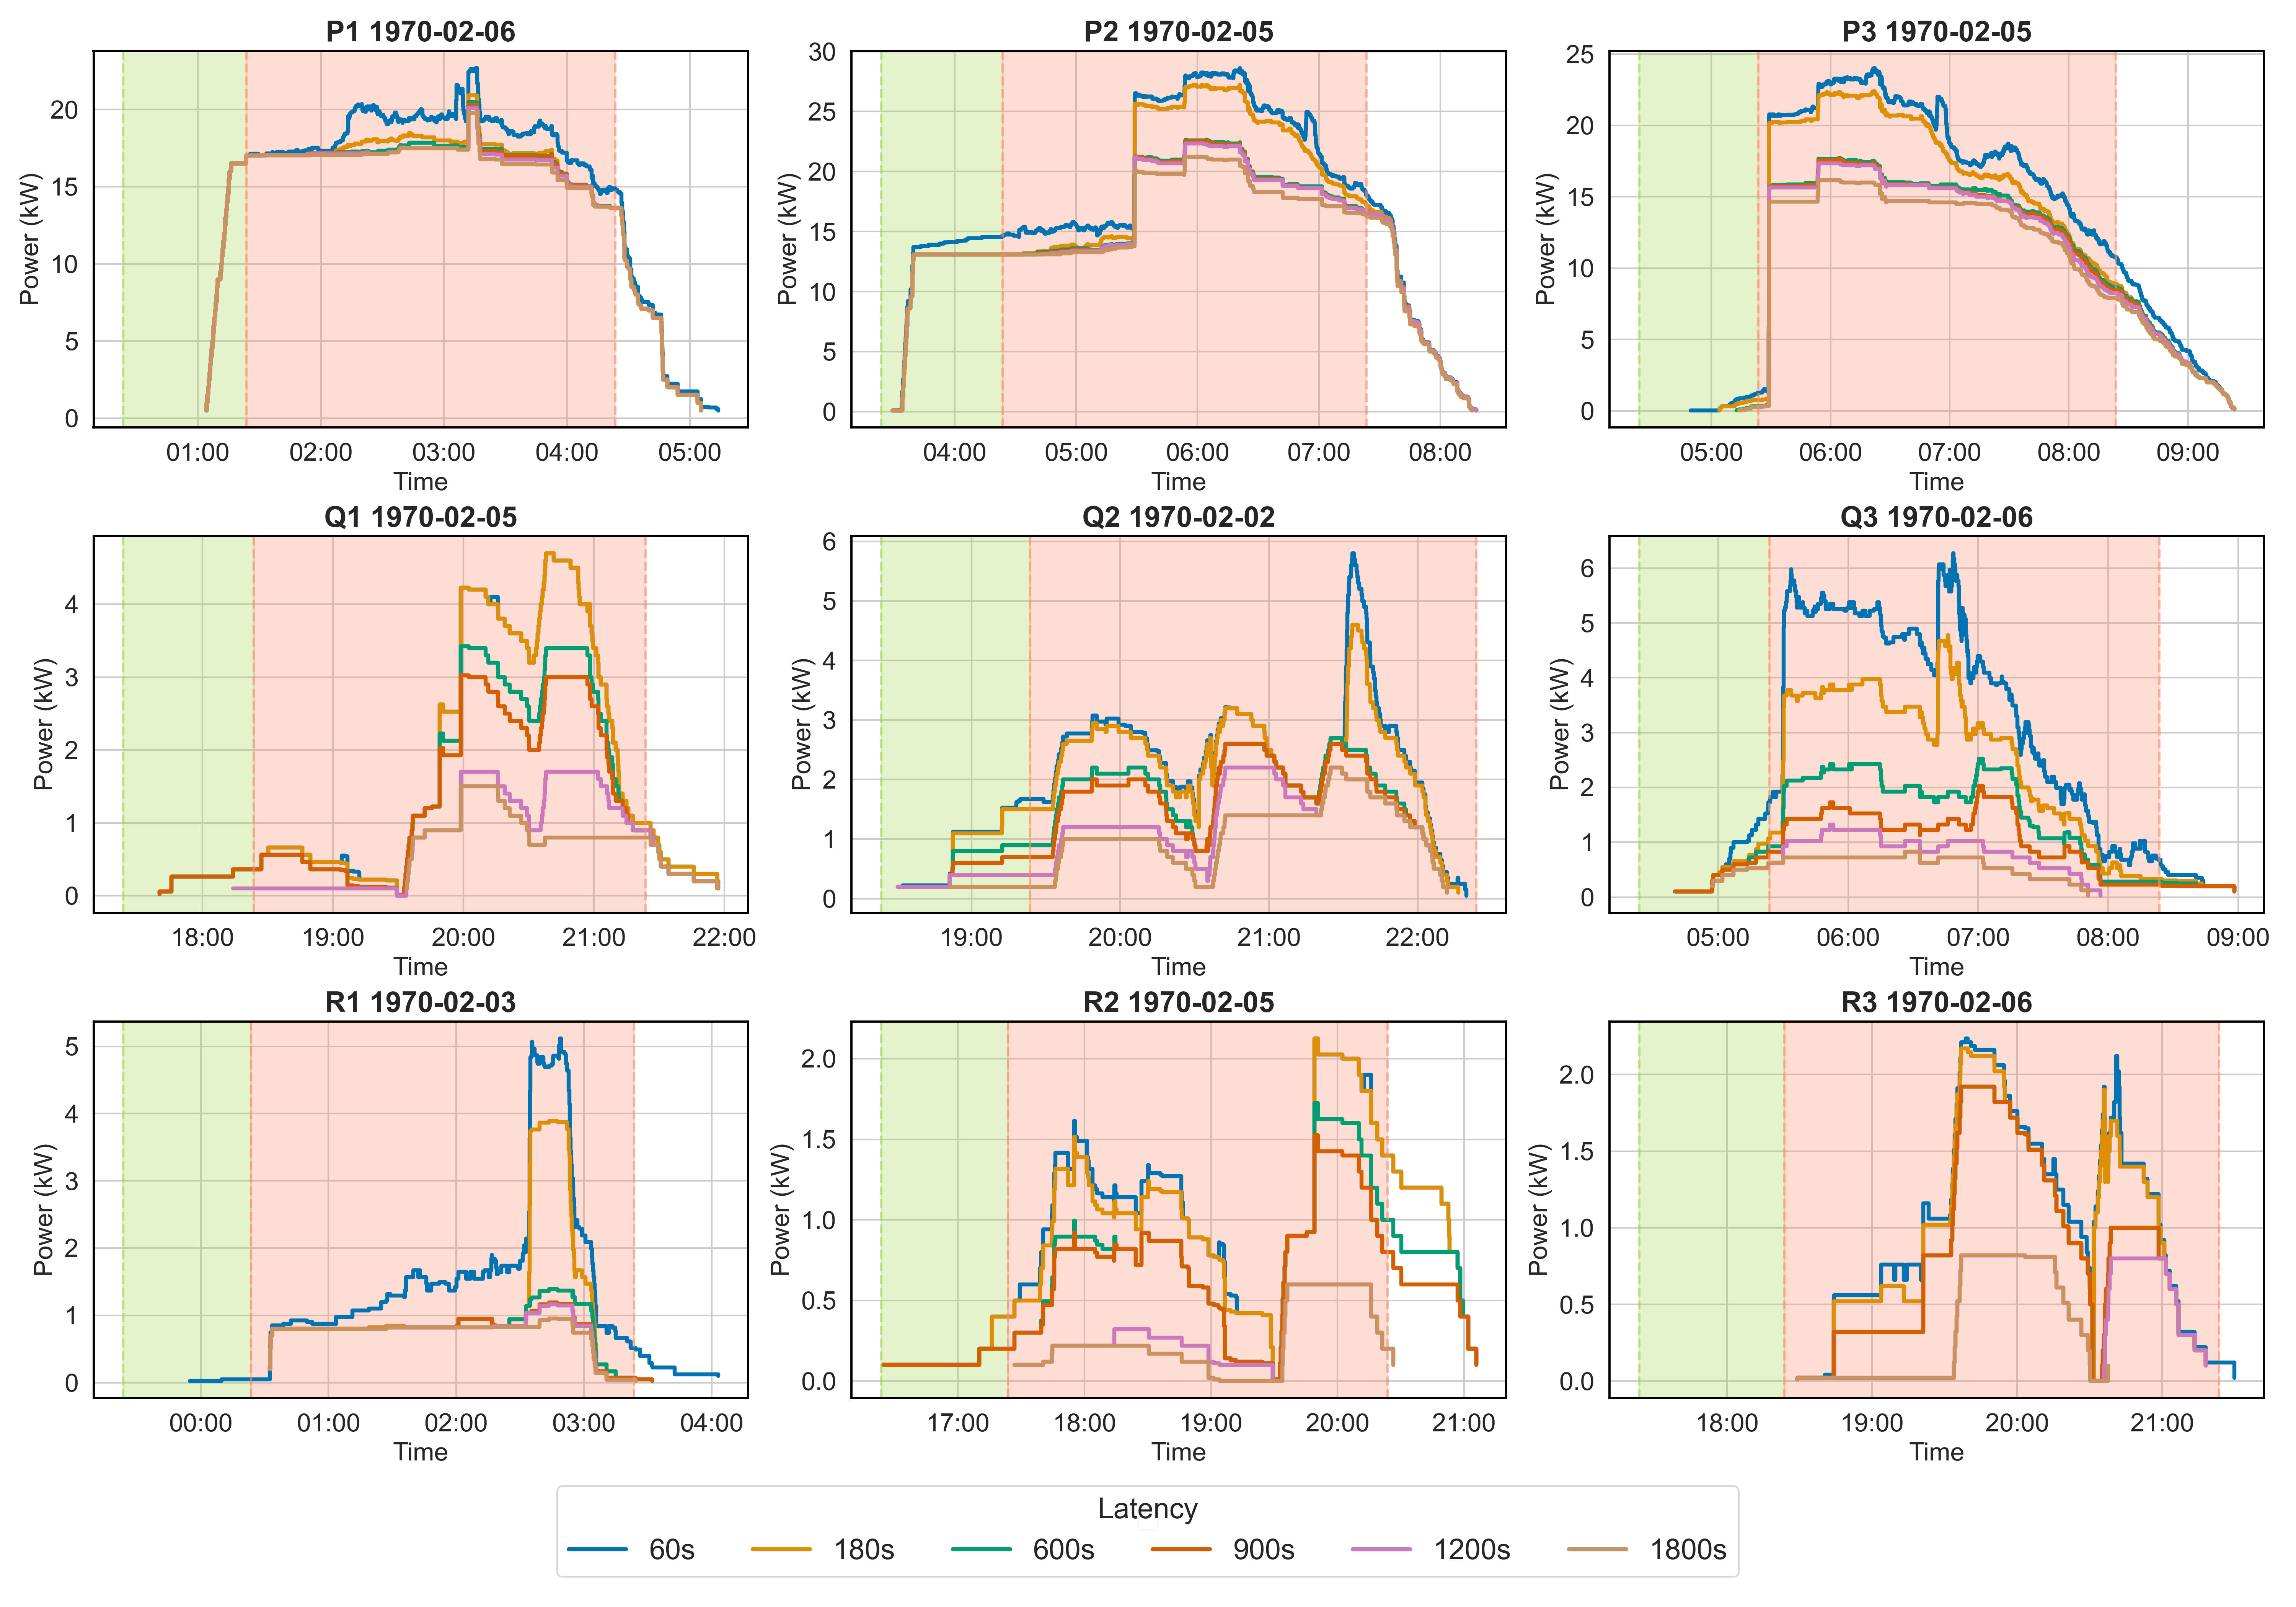
\includegraphics[width=14cm]{sensitivity_grid_fixed_shading_distinct_latencies.png}
    \caption{Sensitivity analysis of deferred power profiles applying LAD-Flex across all points for varying critical latency thresholds.}
    \label{fig:LAD_flex_sens_all}
\end{figure}

The numerical results summarized in Table~\ref{tab:deferrable_energy_latency} confirm the observed trends. Lower latency thresholds correspond to higher deferrable energy, as a larger share of tasks are classified as non-critical and thus eligible for deferral. For instance, at P2, the deferrable energy decreases from 63.88~kWh at $\hat{\lambda} = 60$~s to 44.51~kWh at $\hat{\lambda} = 1800$~s. A similar reduction is observed at P3, with energy dropping from 55.32~kWh to 40.15~kWh. The same trend is present at lower-flexibility points: at Q3, the deferrable energy declines from 10.69~kWh to 1.43~kWh, and at R1, it drops from 4.84~kWh to 2.10~kWh over the same range.

\begin{table}[h!]
\centering
\renewcommand{\arraystretch}{1.2}
\begin{tabular}{@{}c|ccc|ccc|ccc@{}}
\toprule
\textbf{Latency (s)} & \multicolumn{9}{c}{\textbf{Deferrable Energy (kWh)}} \\
                     & P1 & P2 & P3 & Q1 & Q2 & Q3 & R1 & R2 & R3 \\
\midrule
60   & 54.84 & 63.88 & 55.32 & 6.06 & 7.03 & 10.69 & 4.84 & 3.33 & 3.02 \\
180  & 51.76 & 58.29 & 51.32 & 6.04 & 6.56 & 7.62  & 3.29 & 3.19 & 2.85 \\
600  & 51.08 & 50.93 & 43.66 & 4.83 & 5.02 & 4.66  & 2.41 & 2.34 & 2.32 \\
900  & 50.81 & 49.13 & 43.17 & 4.35 & 4.77 & 3.26  & 2.26 & 2.18 & 2.32 \\
1200 & 50.61 & 48.33 & 42.69 & 2.40 & 3.76 & 2.14  & 2.20 & 0.86 & 1.12 \\
1800 & 50.29 & 44.51 & 40.15 & 1.77 & 3.12 & 1.43  & 2.10 & 0.73 & 0.77 \\
\bottomrule
\end{tabular}
\caption{Deferrable energy across different latency threshold settings for each representative point.}
\label{tab:deferrable_energy_latency}
\end{table}

These results demonstrate the strong dependence of LAD-Flex performance on the critical latency threshold. A lower threshold $\hat{\lambda}$ imposes a stricter criterion for classifying tasks as critical, meaning only tasks with very short observed latency are deemed time-sensitive. Consequently, a larger pool of tasks—those with latency exceeding the threshold—become candidates for deferral, increasing the flexibility potential. Conversely, raising the threshold restricts deferrability to tasks with increasingly long latencies, reducing the available flexibility.

Fig.~\ref{fig:LAD_flex_KDE} presents a complementary view through Kernel Density Estimates (KDE) of the deferrable energy distribution across all hourly activations in the sample week, for varying latency thresholds. As expected, lower thresholds shift the distribution toward higher energy values. The distributions are highly skewed with long tails, indicating that under favorable workload conditions, the DC can deliver substantial flexibility. However, the bulk of instances are concentrated at lower energy values.

Importantly, the distributions remain strictly above zero across all considered latency thresholds, confirming that LAD-Flex consistently identifies non-zero flexibility potential even under more restrictive parameter settings. This reinforces the reliability of the strategy across a range of operational configurations.

\begin{figure}[!h]
    \centering
    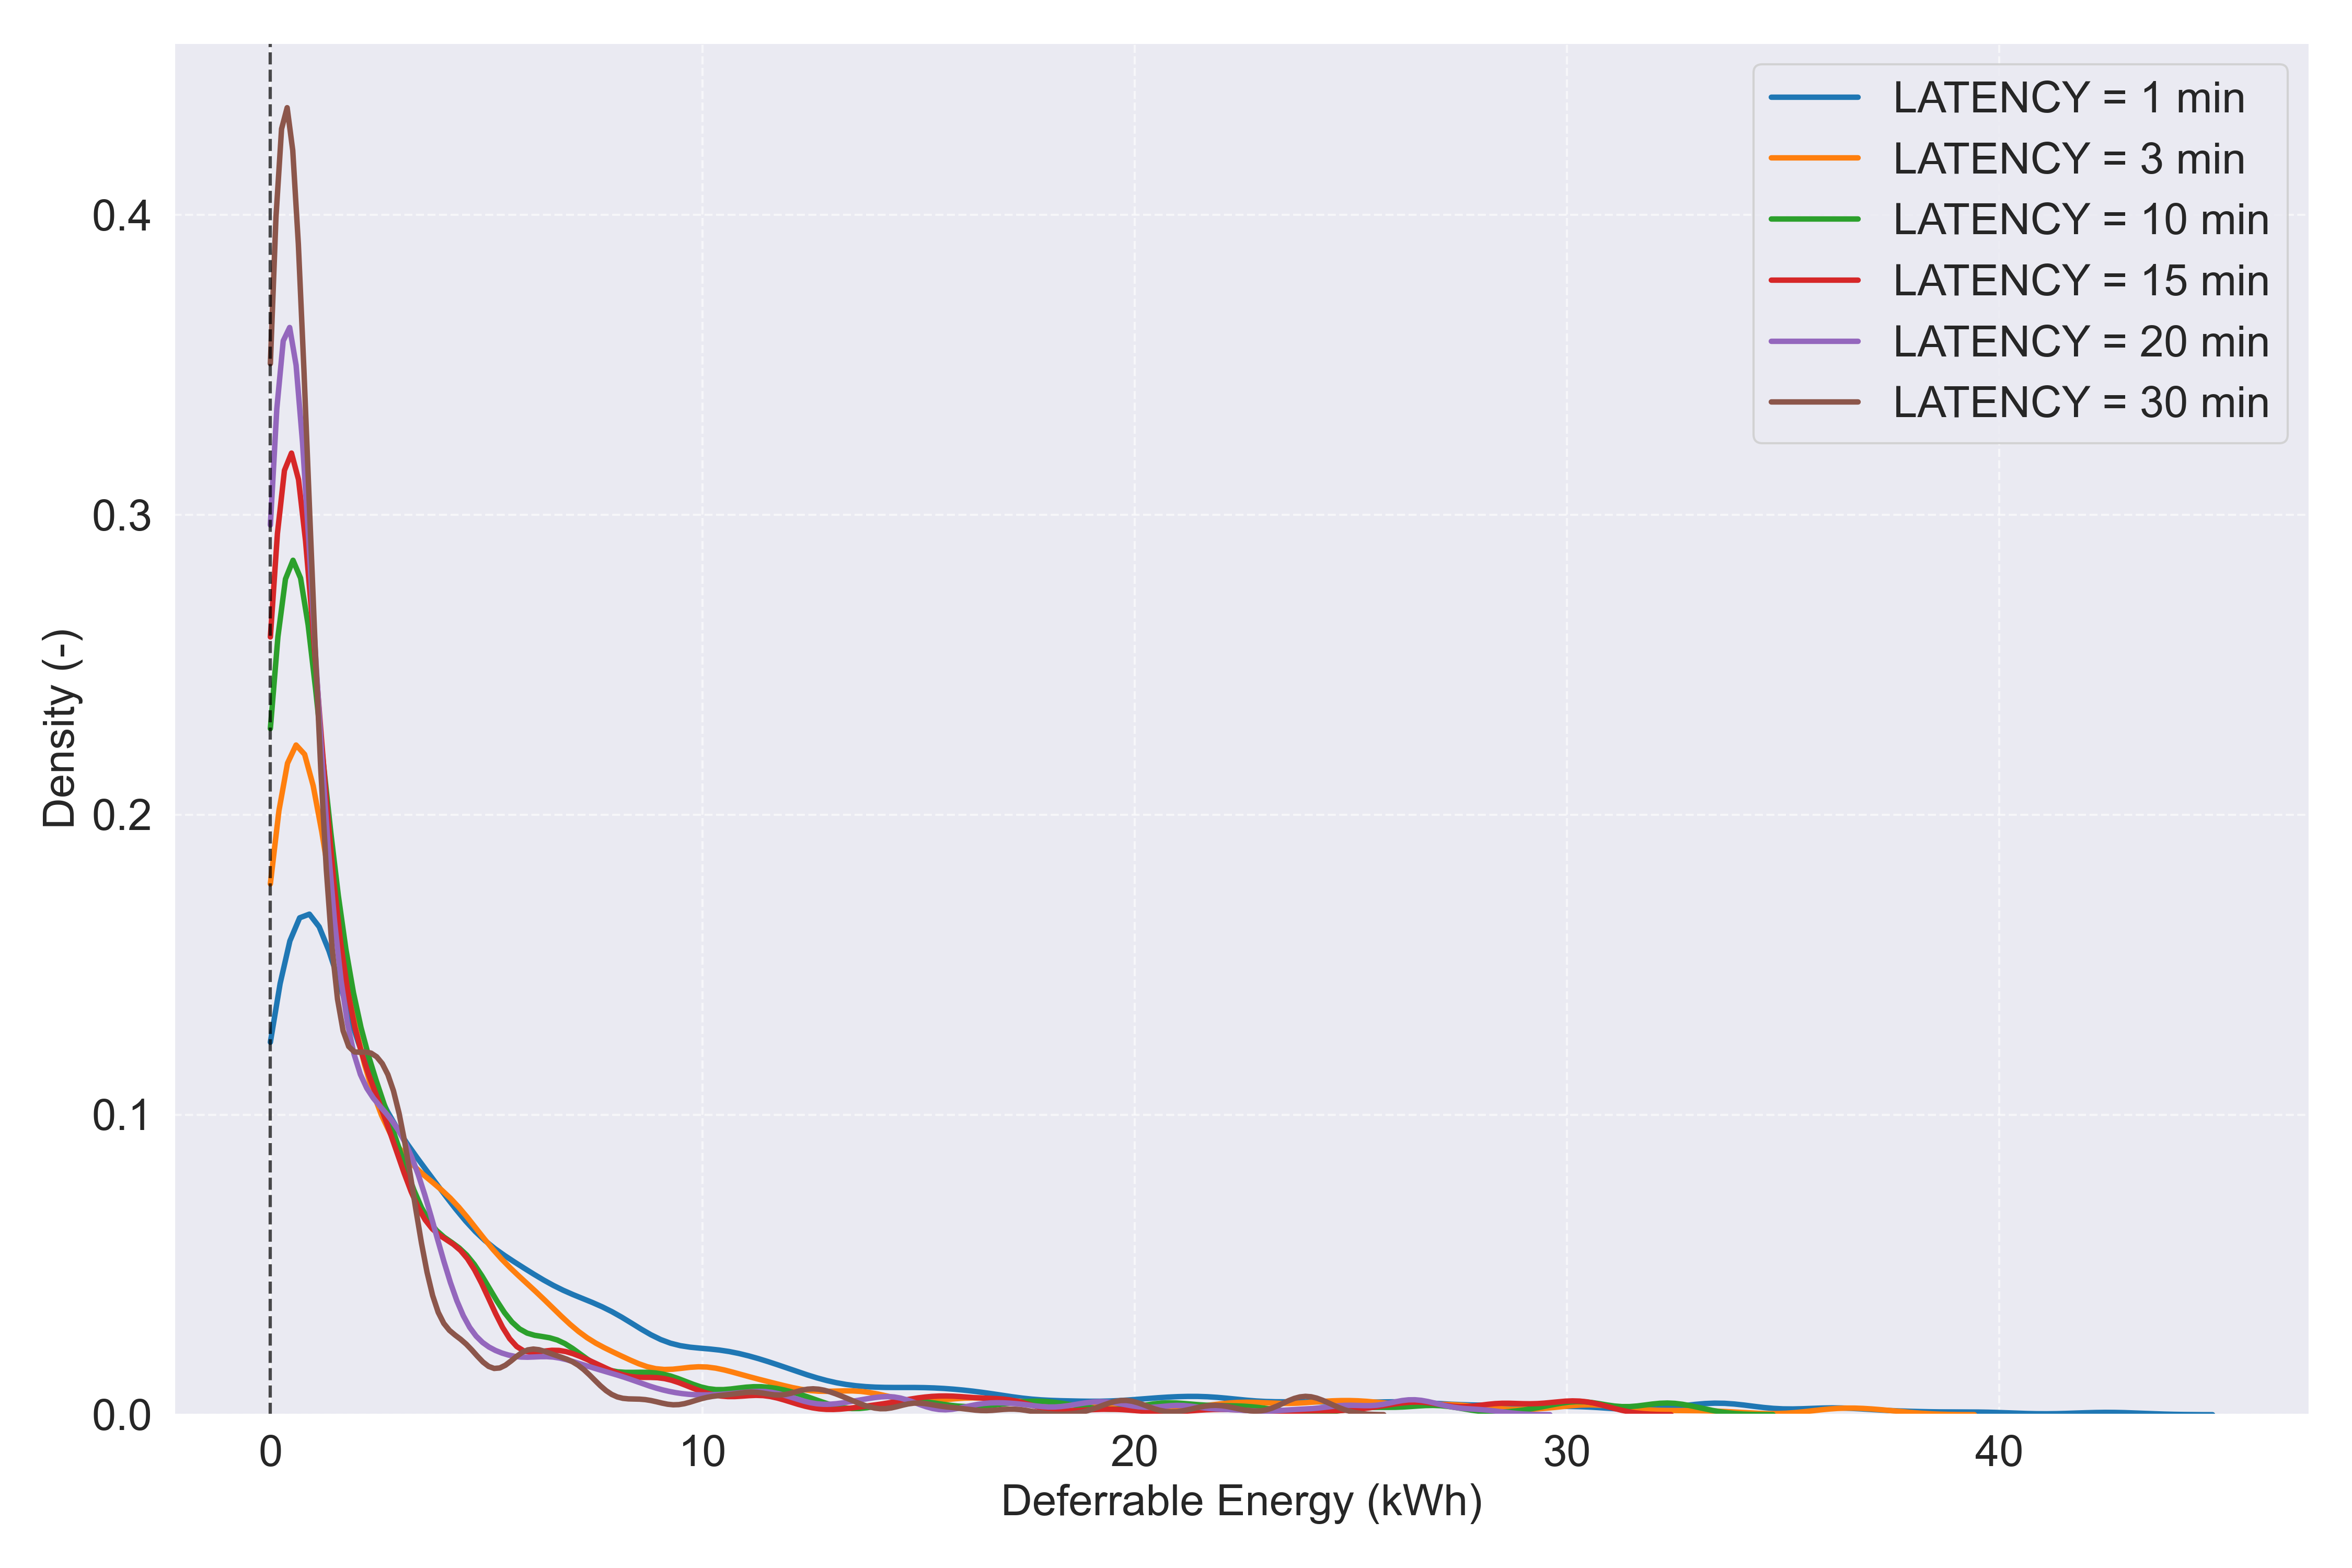
\includegraphics[width=14cm]{sensitivity_KDE_latency_filtered_improved.png}
    \caption{KDE plot of deferrable energy distribution over the sample week for different values of critical latency threshold.}
    \label{fig:LAD_flex_KDE}
\end{figure}


%%%%%%%%%%%%%%%%%%%%%%%%%%%%%%%%%%%%%%%%%%%%%%%%%%%%%%%%%%%%%%%%%%%%%%%%%%%%%%%
\subsubsection{Robustness Analysis Under Duration Prediction Uncertainty} \label{sec:robustness}
%%%%%%%%%%%%%%%%%%%%%%%%%%%%%%%%%%%%%%%%%%%%%%%%%%%%%%%%%%%%%%%%%%%%%%%%%%%%%%%

The results presented in Section~\ref{LAD_flex_results} assume perfect knowledge of task durations, representing an idealized upper bound on LAD-Flex performance. In practice, however, task duration prediction is subject to uncertainty, as discussed in Section~\ref{prediction_uncertainty_methods}. This section evaluates the robustness of the strategy under realistic operational conditions by analyzing performance when task durations are predicted with varying levels of error.

Following the stochastic model outlined in Section~\ref{prediction_uncertainty_methods}, predicted task durations $\hat{d}_k$ are modeled as:
\begin{equation}
\hat{d}_k = d_k + \varepsilon_k, \quad \text{where} \quad \varepsilon_k \sim \mathcal{N}(0, (\zeta \cdot d_k)^2)
\end{equation}

\noindent Three prediction error levels are considered, as summarized in Table~\ref{tab:prediction_error_scenarios}.

\begin{table}[htbp]
\centering
\caption{Prediction error scenarios for robustness analysis.}
\label{tab:prediction_error_scenarios}
\begin{tabular}{@{}lc@{}}
\toprule
\textbf{Uncertainty Level} & $\zeta$ \\
\midrule
Perfect Information & 0.0 \\
Low Uncertainty & 0.1 \\
Moderate Uncertainty & 0.3 \\
High Uncertainty & 0.5 \\
\bottomrule
\end{tabular}
\end{table}

The $\zeta = 0.3$ scenario approximates realistic prediction performance, as the publishers of the trace report MAE below 25\% for 78\% of recurring tasks~\cite{Weng2022}. The $\zeta = 0.1$ and $\zeta = 0.5$ scenarios bound this realistic case under optimistic and pessimistic prediction capabilities, respectively.

Fig.~\ref{fig:prediction_error_distribution} characterizes the prediction errors across the three uncertainty scenarios. Panel (a) shows the probability density of prediction errors expressed as percentage deviations from true duration; higher values of $\zeta$ result in wider error distributions. Panel (b) presents a scatter plot of actual versus predicted task duration for the worst-case scenario ($\zeta = 0.5$). While the relative prediction error is substantial, the vast majority of tasks considered for flexibility provision have relatively short durations. This concentration means that even large percentage errors translate to relatively small absolute deviations. Furthermore, the LAD-Flex strategy automatically excludes tasks significantly longer than the flexibility window, limiting exposure to prediction errors on long-duration tasks.

\begin{figure}[htbp]
\centering
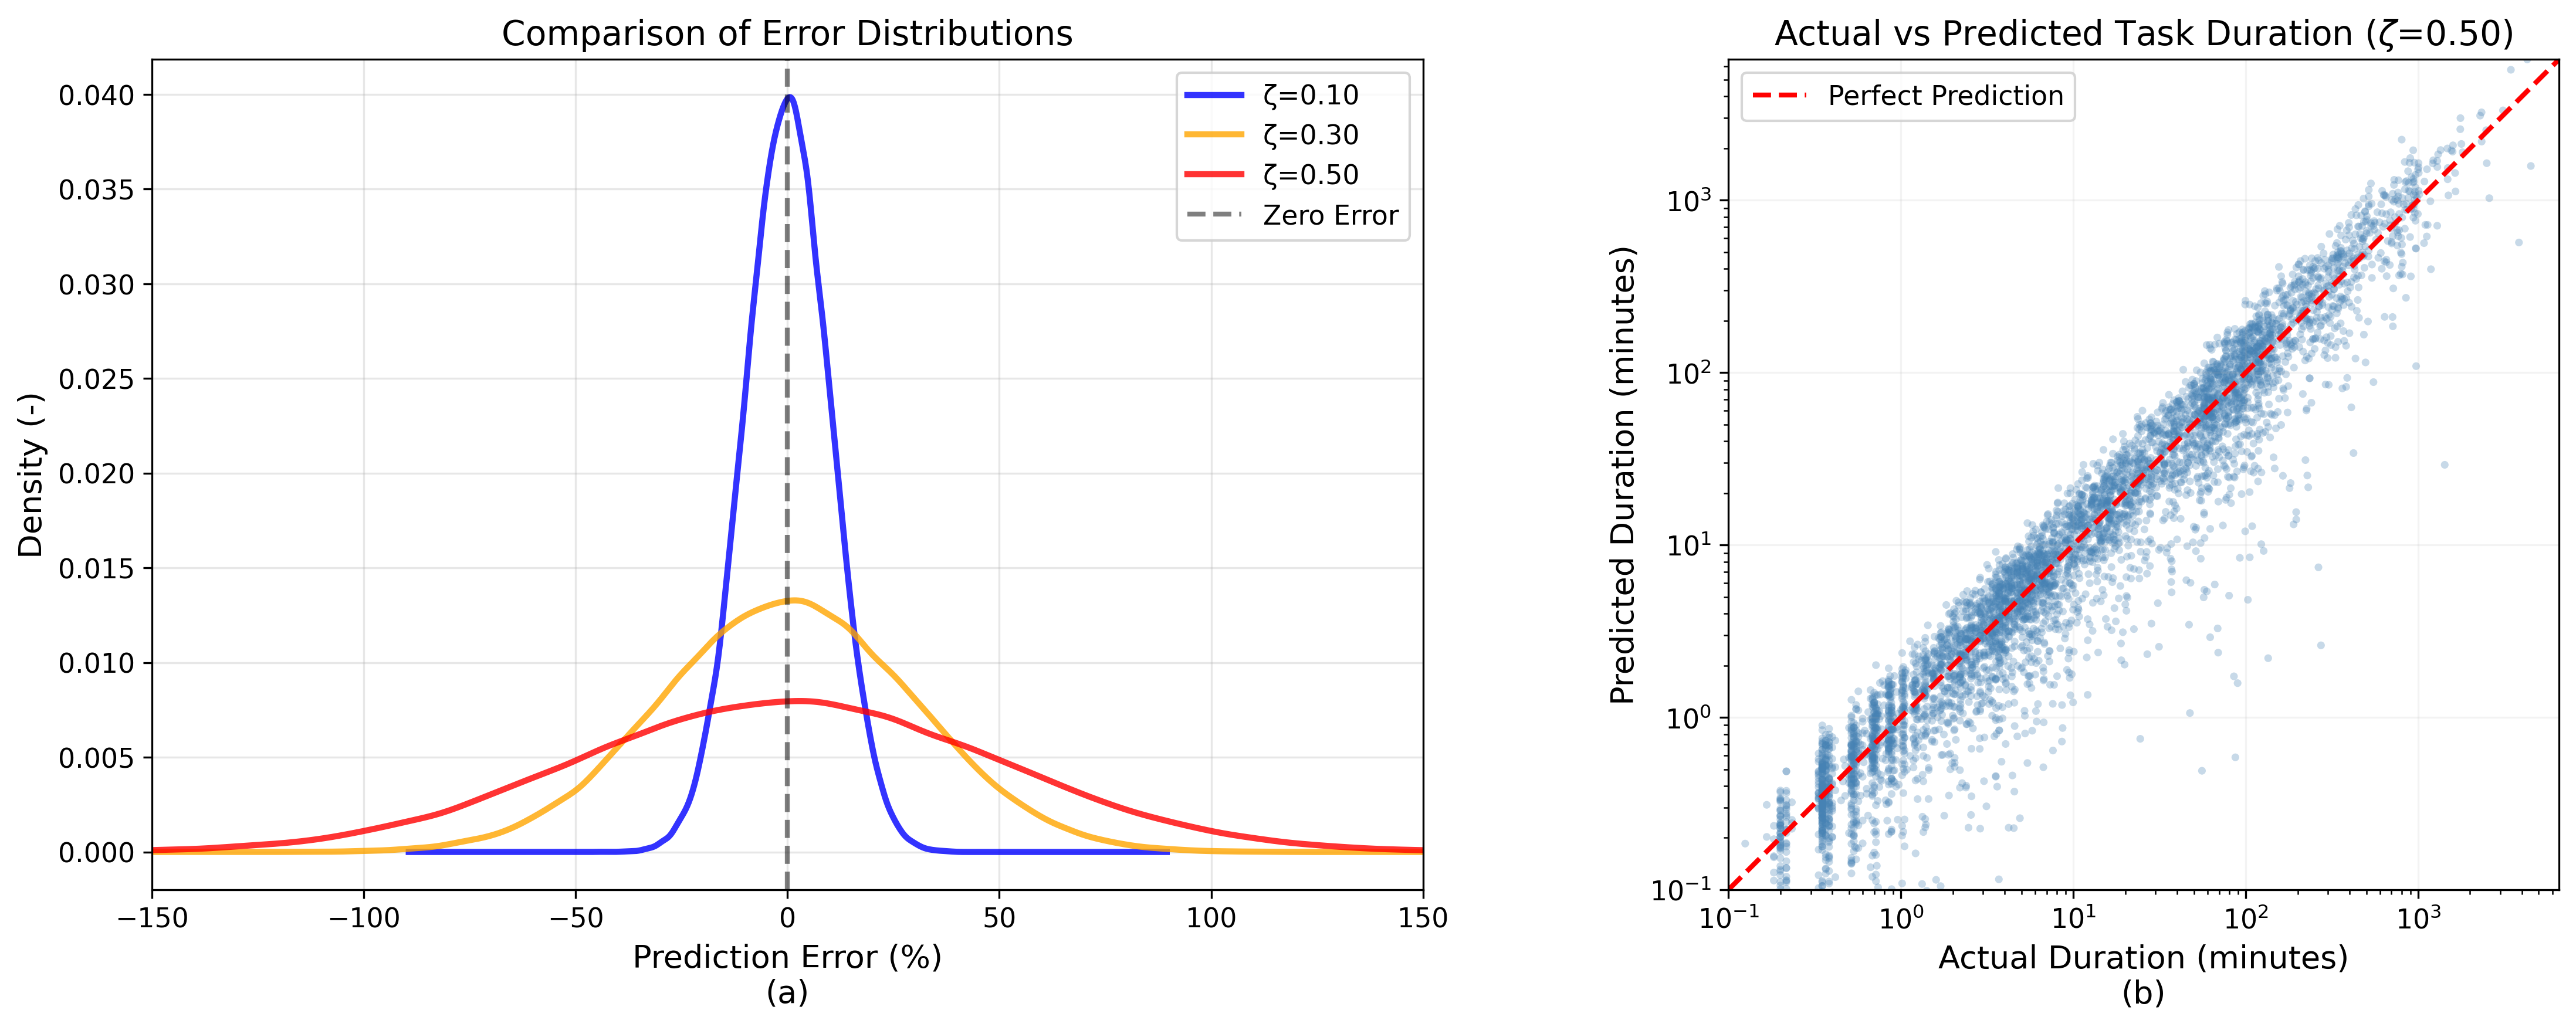
\includegraphics[width=\textwidth]{error_and_scatter_combined_zeta_010_030_050_loglog.png}
\caption{Characterization of duration prediction errors: (a) Probability density of prediction errors for different values of $\zeta$. (b) Scatter plot of actual vs.\ predicted task duration for the $\zeta = 0.5$ scenario.}
\label{fig:prediction_error_distribution}
\end{figure}

Fig.~\ref{fig:3x3_gamma_effect} illustrates how prediction uncertainty affects deferred power profiles across the nine representative points. At high-flexibility points (P1–P3), the deferred power profiles exhibit remarkable stability across all uncertainty levels. Even at $\zeta = 0.5$, the profiles deviate only slightly from the perfect-information baseline, with minor reductions in peak deferred power. Similar robustness is observed for mid-range (Q1–Q3) and median (R1–R3) points. In all cases, the overall shape and timing of deferred power profiles remain consistent, confirming that LAD-Flex decision logic is resilient to imperfect duration predictions.

\begin{figure}[htbp]
\centering
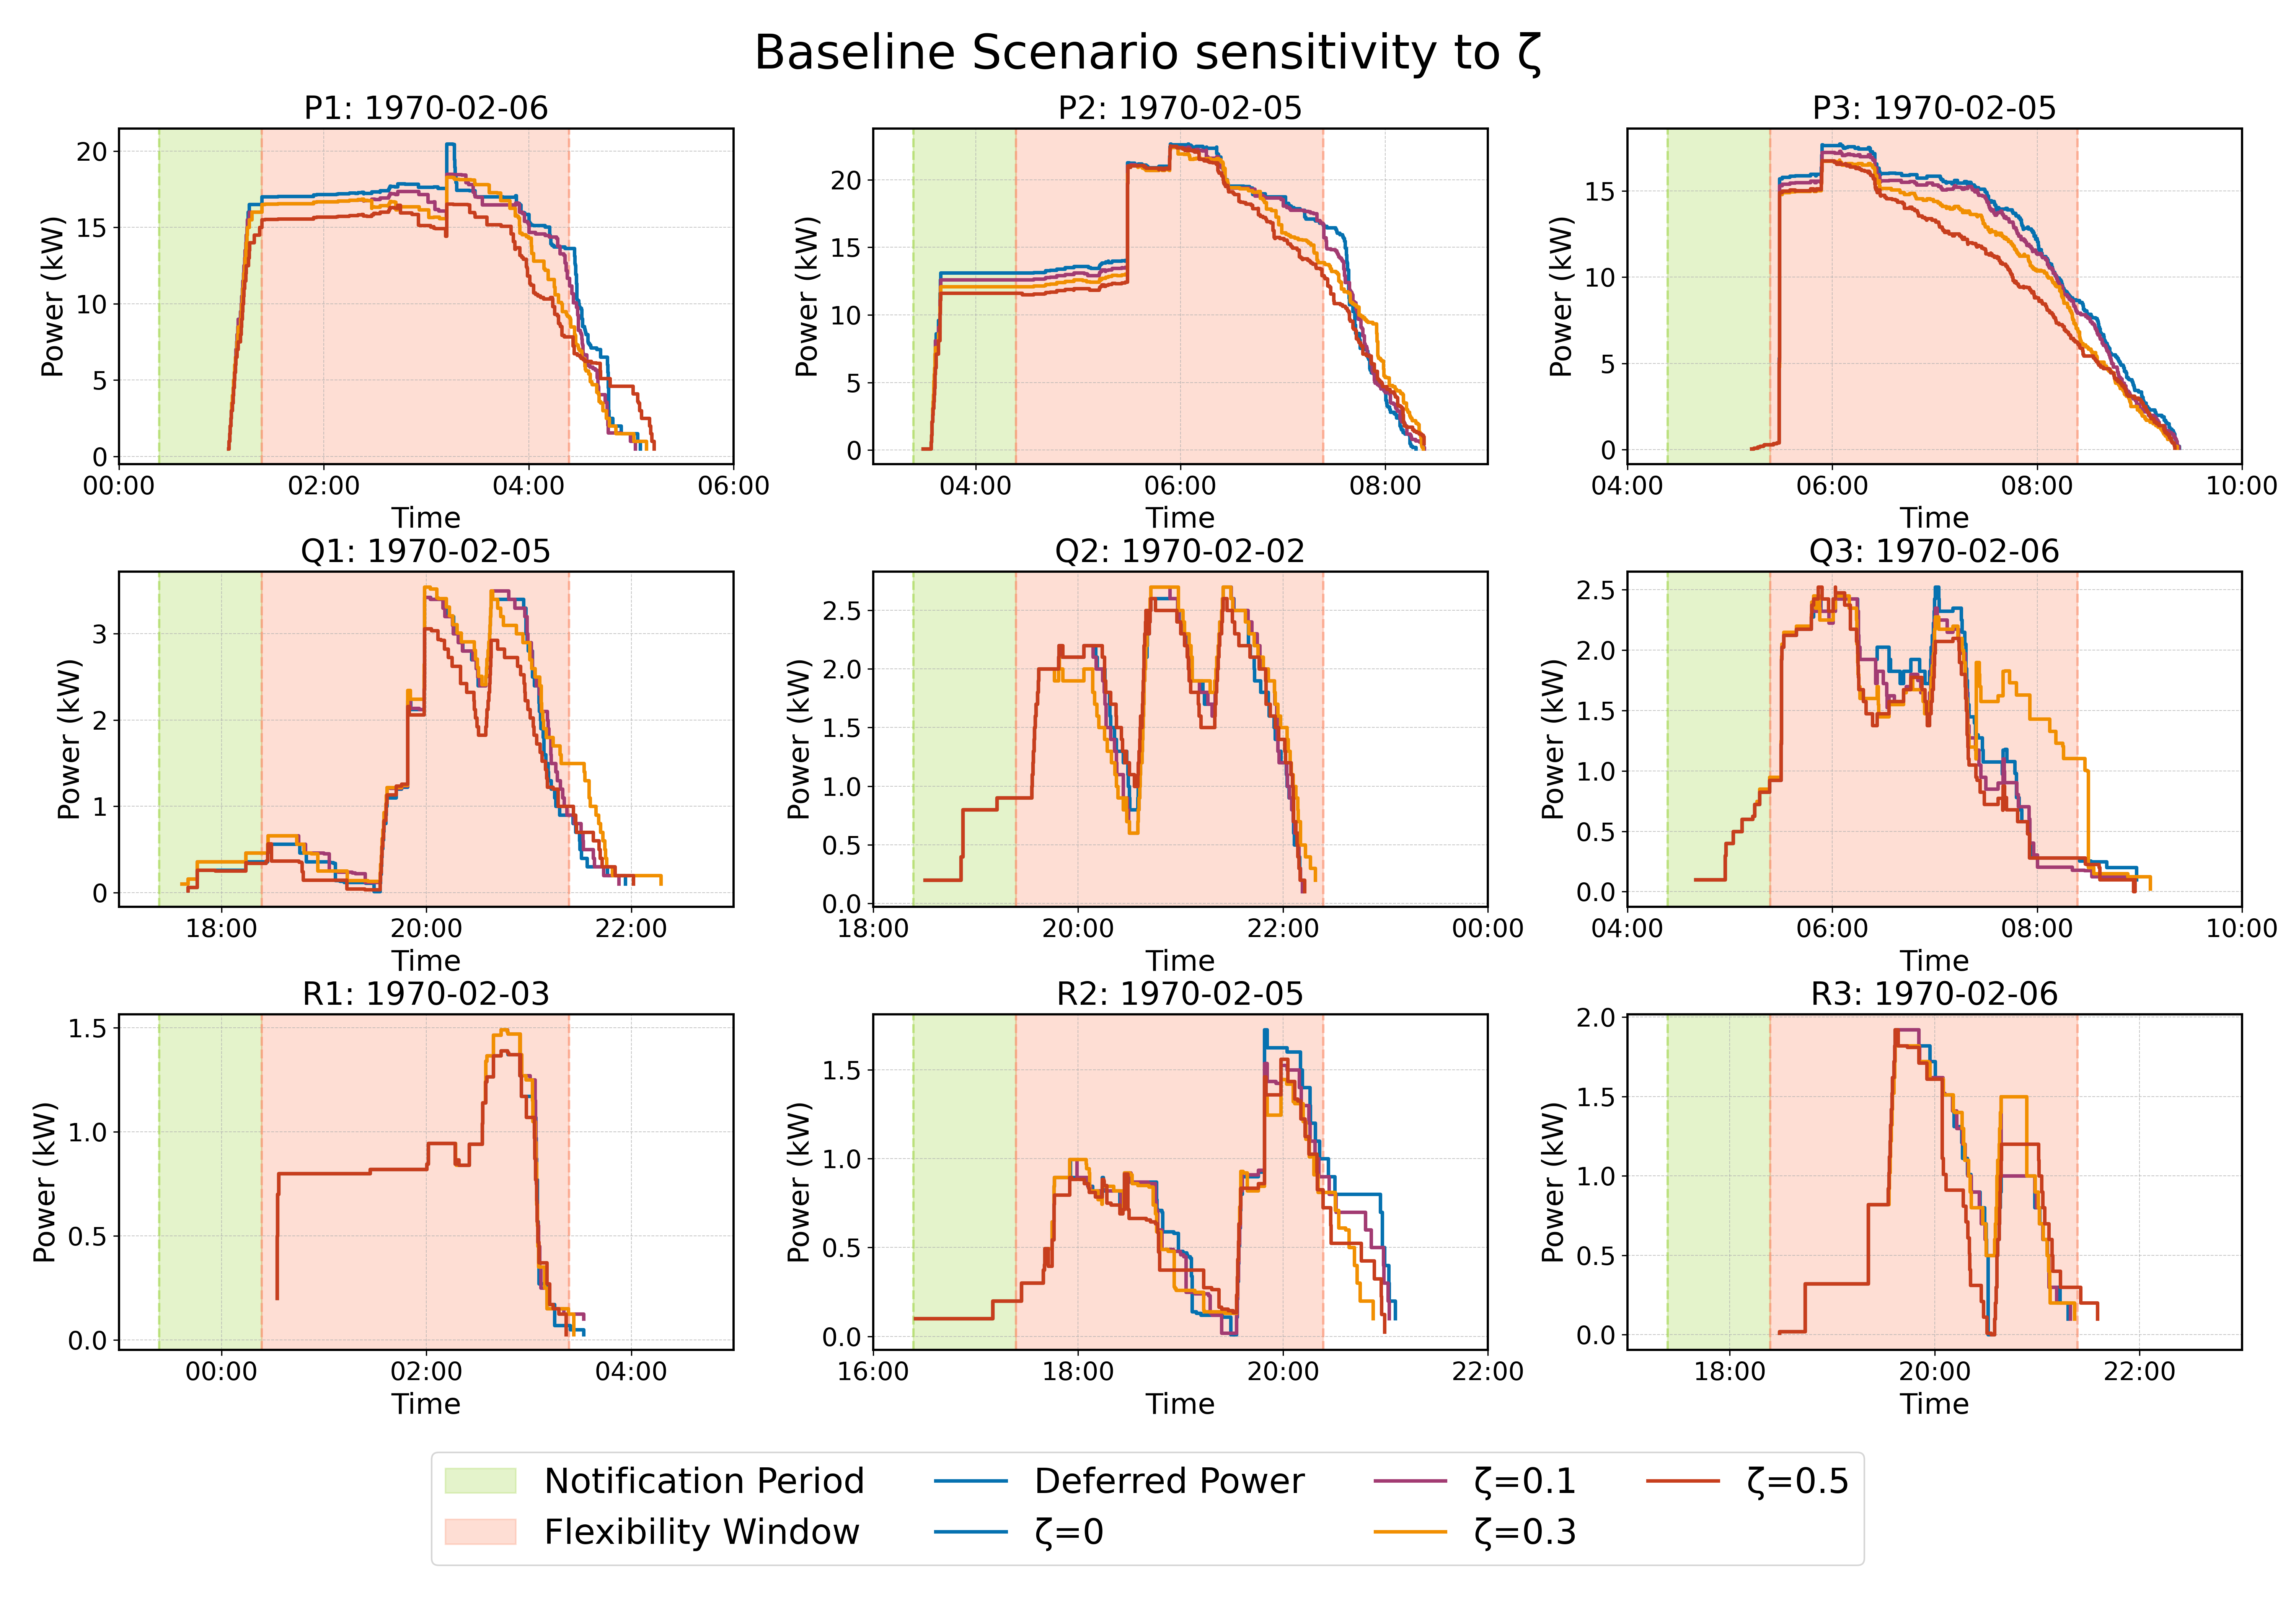
\includegraphics[width=\textwidth]{deferred_power_timeseries_3x3_zeta_DEFAULT_BASELINE.png}
\caption{Effect of duration prediction uncertainty on deferred power profiles for the nine representative points.}
\label{fig:3x3_gamma_effect}
\end{figure}

To quantify how prediction errors affect task deferral decisions, Fig.~\ref{fig:confusion_matrices} presents confusion matrices comparing task classifications under uncertain predictions against the perfect-information baseline. Each matrix compares deferral decisions at a given $\zeta$ level with those at $\zeta = 0$: true positives (top-left) are tasks correctly identified as deferrable under both conditions; false negatives (top-right) are tasks rejected under uncertainty that would have been deferred with perfect information; false positives (bottom-left) are tasks deferred under uncertainty that would have been rejected; and true negatives (bottom-right) are tasks correctly identified as non-deferrable in both cases.

\begin{figure}[htbp]
\centering
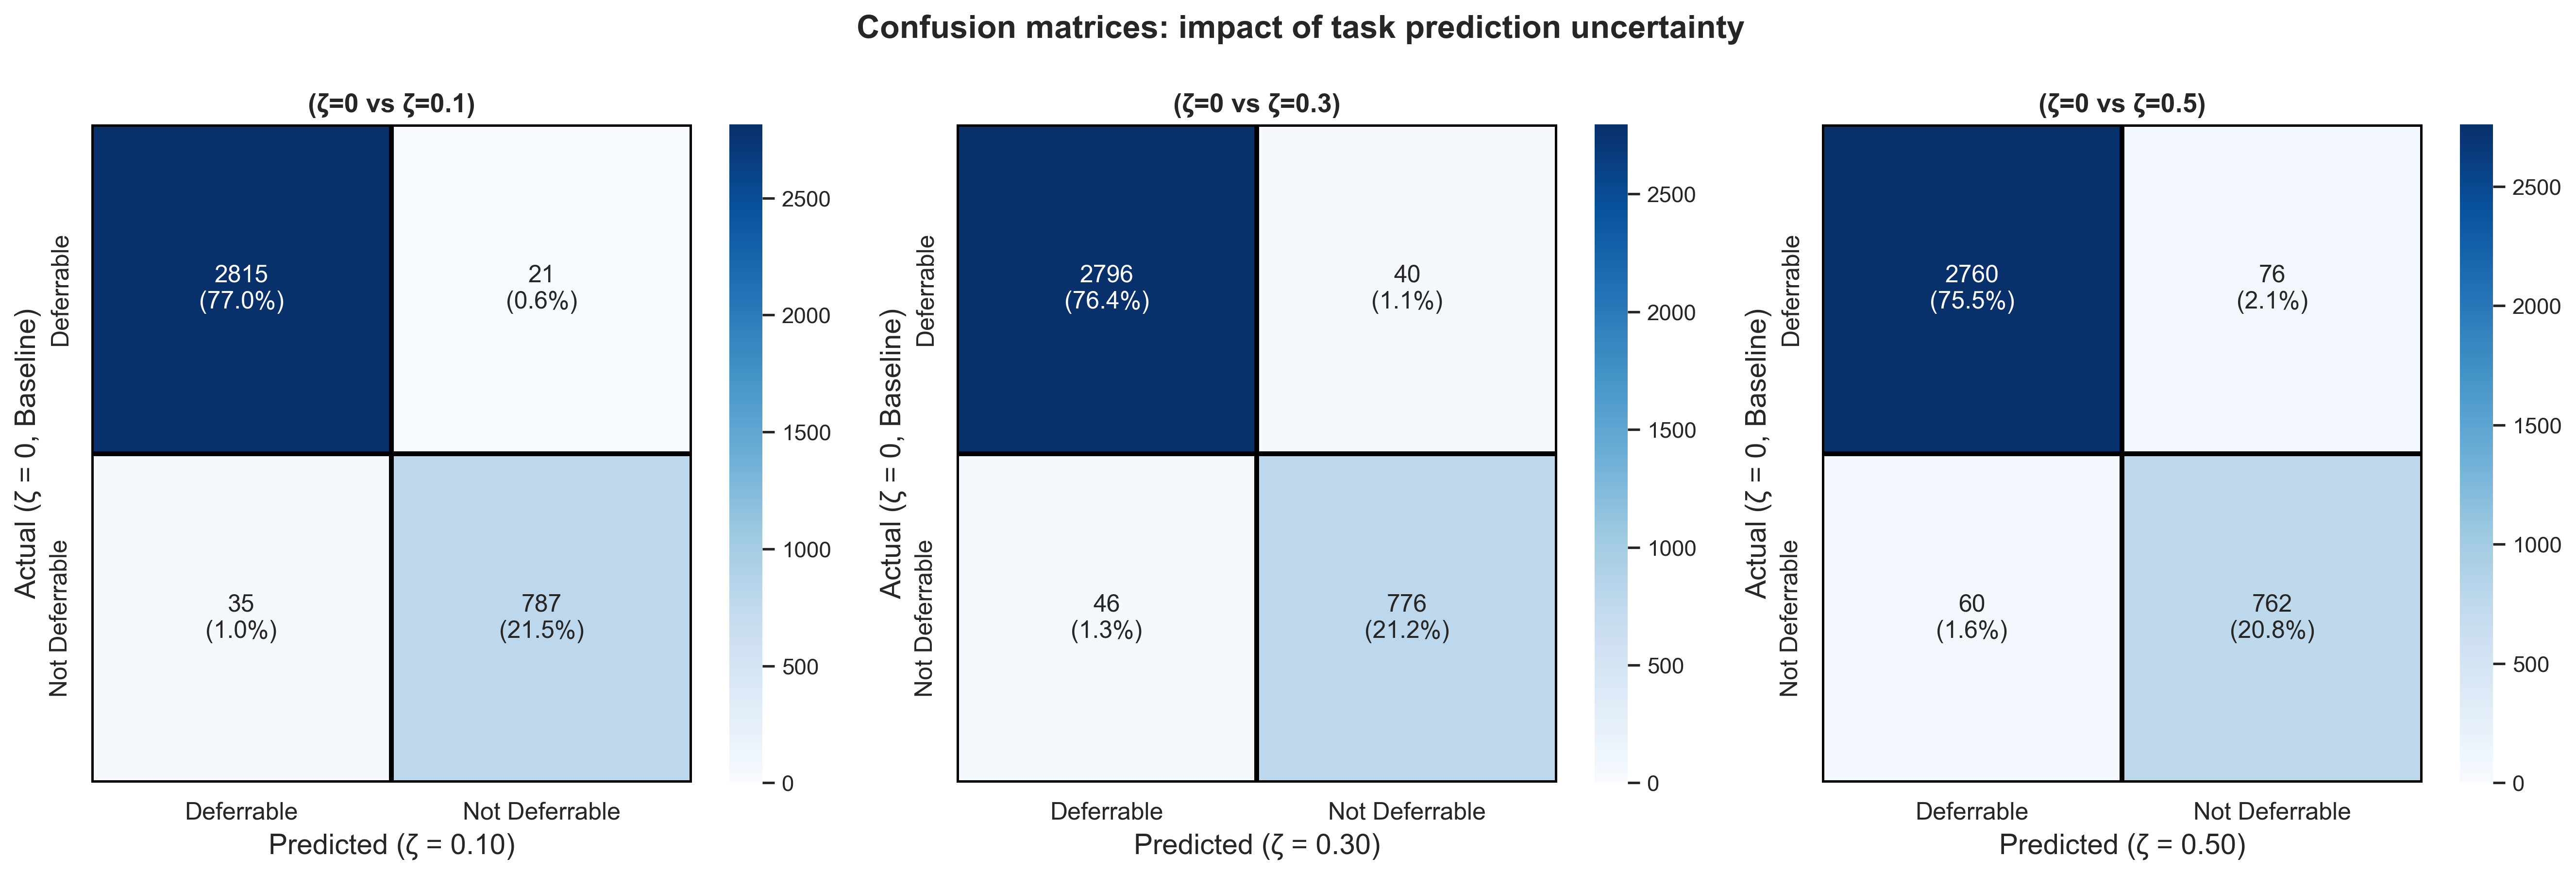
\includegraphics[width=\textwidth]{confusion_matrix_zeta_comparison_DEFAULT_BASELINE.png}
\caption{Confusion matrices comparing task deferrability classifications under prediction uncertainty against the perfect-information baseline.}
\label{fig:confusion_matrices}
\end{figure}

The results demonstrate strong classification stability. At low uncertainty ($\zeta = 0.1$), accuracy reaches 98.5\% with negligible misclassification. Under moderate uncertainty ($\zeta = 0.3$), accuracy remains high at 97.6\%, with only a modest increase in false negatives. Even at high uncertainty ($\zeta = 0.5$), accuracy degrades only slightly to 96.3\%, while precision and recall remain above 97\%.

This robustness arises from two factors. First, most tasks eligible for flexibility provision have short durations, so even large relative errors translate into modest absolute deviations. Second, the overhang tolerance ($\beta_{\text{overhang}} = 0.7$) and buffer period ($\gamma_{\text{buffer}} = 60$~min) act as built-in safety margins: underestimation of task duration is mitigated by the buffer beyond the flexibility window, while overestimation is absorbed by the allowable overhang. This mechanism keeps both false positives and false negatives low across all uncertainty levels.

In summary, the robustness analysis confirms that LAD-Flex maintains reliable performance under realistic prediction uncertainty. The strategy's conservative parameter design—incorporating overhang tolerance and buffer periods—provides inherent resilience against duration estimation errors, ensuring operational viability without requiring highly accurate prediction models. Combined with the sensitivity analysis, these results establish that LAD-Flex can be deployed across a range of parameter configurations and prediction capabilities while consistently delivering actionable flexibility for grid services. 





























































\subsection{Notification period optimization} \label{notification_results}

This section presents the results of the notification period optimization, as introduced in Section~\ref{notification_period_opt_section_methodology}. The combinations of $(\tau, \alpha)$ considered in this section represent sensitivity scenarios, with the purpose of evaluating whether the optimal notification strategy remains robust across a range of plausible value-decay profiles. The analysis is carried out assuming a threshold latency of $\hat{\lambda} = 10$ minutes and an effective flexibility window of $\eta \Delta T = 3$ hours. The value of flexibility, $V(\delta)$, is taken from the parametrization shown in Fig.~\ref{fig:flex_value_vs_time}.

For a discrete range of notification times $\delta$, both the flexible energy $F(\delta)$ and the resulting revenue $R(\delta) = F(\delta) \cdot V(\delta)$ are computed across all combinations of the parameters ($\alpha$) and ($\tau$). This computation is repeated for all the notable time points identified previously. The results are shown graphically in Fig.~\ref{fig:opt_results_sensitive}.

Interestingly, in several cases (P1, Q3, R1, R3), the flexible energy $F(\delta)$ remains constant regardless of the notification period. This indicates that increasing $\delta$ does not enable the DC to reschedule additional flexible tasks. For such cases, it is therefore more advantageous to provide real-time flexibility to the aggregator, rather than delaying commitment.

\begin{figure}[!h]
    \centering
    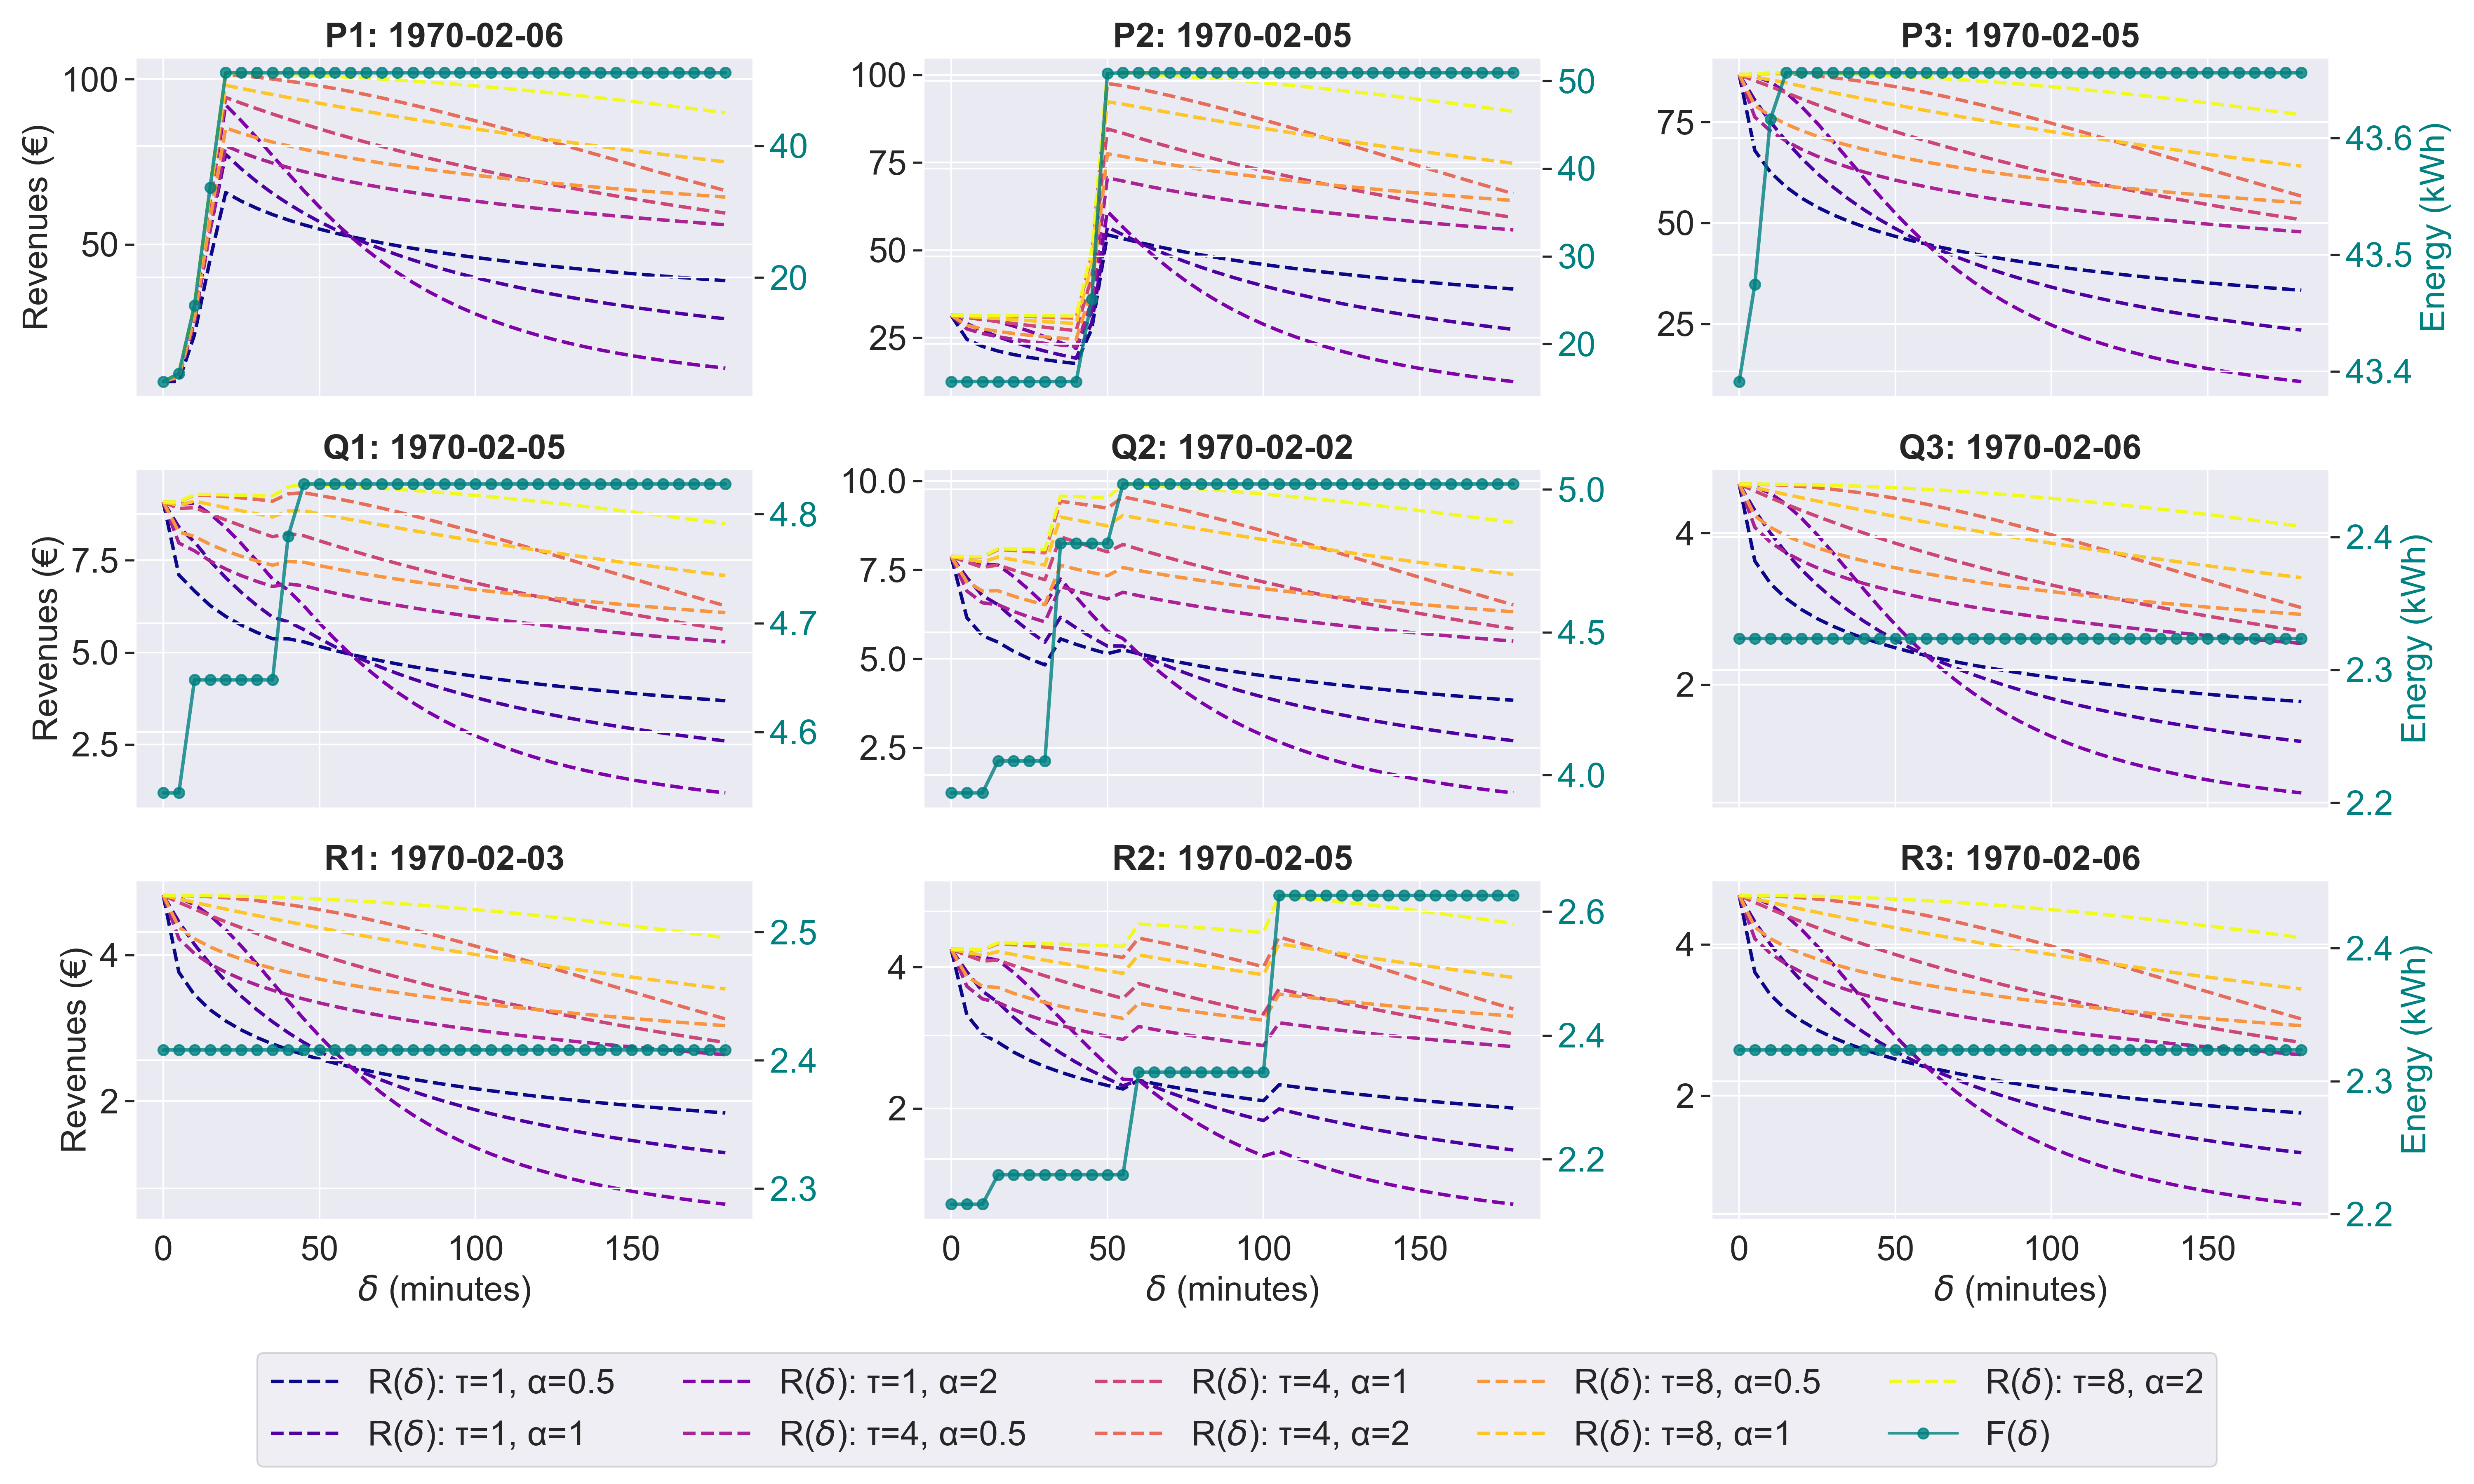
\includegraphics[width=17cm]{flexibility_sensitivity_all_points_impr_clean.png}
    \caption{Revenues $R(\delta)$ and flexibility amount $F(\delta)$ for different notification periods \( \delta \) across selected evaluation points}
\label{fig:opt_results_sensitive}
\end{figure}

To summarize how different points can assume different values of $\delta^*$, Table~\ref{tab:opt_delta_and_revenue_transposed} shows the results for the different combinations of parameters across the chosen points. In general, both the optimal notification period $\delta^*$ and the resulting revenue $R$ tend to increase with higher values of the scale parameter $\tau$, which broadens the value function over time. A similar, though less pronounced, effect is observed with increasing shape parameter $\alpha$, especially at lower values of $\tau$.

For certain points (e.g., Q1 and Q2), the increase in $\tau$ leads to a clear shift of $\delta^*$ toward higher values (up to 55 minutes), reflecting a trade-off between scheduling flexibility and the decreasing value of delayed activation. Conversely, for other points (e.g., Q3, R1, and R3), the optimal $\delta^*$ remains constant at zero across all parameter settings, confirming that the available flexibility does not increase with more advanced notice. These points correspond to operating conditions where flexibility is either fully available immediately or not affected by the notification time.

Despite the variability, all combinations yield strictly positive revenue, reaffirming that the LAD-Flex strategy is consistently able to activate flexibility, even when constrained by higher notification periods or less favorable valuation functions.

\begin{table}[h!]
\centering
\scriptsize
\renewcommand{\arraystretch}{1.15}
\setlength{\tabcolsep}{4pt}
\resizebox{\dimexpr\textwidth+32pt}{!}{
\begin{tabular*}{\textwidth}{@{\extracolsep{\fill}}l*{9}{p{0.4cm} p{0.48cm}}@{}}
\toprule
\diagbox[width=4.8em]{\((\tau,\alpha)\)}{Point}
& \multicolumn{2}{c}{P1} & \multicolumn{2}{c}{P2} & \multicolumn{2}{c}{P3}
& \multicolumn{2}{c}{Q1} & \multicolumn{2}{c}{Q2} & \multicolumn{2}{c}{Q3}
& \multicolumn{2}{c}{R1} & \multicolumn{2}{c}{R2} & \multicolumn{2}{c}{R3} \\
\midrule
& $\delta^*$ & R & $\delta^*$ & R & $\delta^*$ & R 
& $\delta^*$ & R & $\delta^*$ & R & $\delta^*$ & R 
& $\delta^*$ & R & $\delta^*$ & R & $\delta^*$ & R \\
& (min) & (€) & (min) & (€) & (min) & (€) 
& (min) & (€) & (min) & (€) & (min) & (€) 
& (min) & (€) & (min) & (€) & (min) & (€) \\
\midrule
(1,0.5) & 20 & 65.7 & 50 & 54.3 & 0 & 86.7 & 0 & 9.1 & 0 & 7.8 & 0 & 4.6 & 0 & 4.8 & 0 & 4.2 & 0 & 4.6 \\
(1,1)   & 20 & 77.2 & 50 & 56.6 & 0 & 86.7 & 0 & 9.1 & 0 & 7.8 & 0 & 4.6 & 0 & 4.8 & 0 & 4.2 & 0 & 4.6 \\
(1,2)   & 20 & 92.1 & 50 & 61.0 & 0 & 86.7 & 0 & 9.0 & 0 & 7.8 & 0 & 4.6 & 0 & 4.8 & 0 & 4.2 & 0 & 4.6 \\
(4,0.5) & 20 & 79.8 & 50 & 70.6 & 0 & 86.7 & 0 & 9.1 & 0 & 7.8 & 0 & 4.6 & 0 & 4.8 & 0 & 4.2 & 0 & 4.6 \\
(4,1)   & 20 & 94.4 & 50 & 84.5 & 0 & 86.7 & 0 & 9.0 & 35 & 8.4 & 0 & 4.6 & 0 & 4.8 & 0 & 4.2 & 0 & 4.6 \\
(4,2)   & 20 & 101.4 & 50 & 97.5 & 10 & 87.0 & 45 & 9.3 & 55 & 9.5 & 0 & 4.6 & 0 & 4.8 & 105 & 4.4 & 0 & 4.6 \\
(8,0.5) & 20 & 85.2 & 50 & 77.4 & 0 & 86.7 & 0 & 9.1 & 0 & 7.8 & 0 & 4.6 & 0 & 4.8 & 0 & 4.5 & 0 & 4.6 \\
(8,1)   & 20 & 98.1 & 50 & 92.3 & 0 & 86.7 & 10 & 9.1 & 55 & 9.0 & 0 & 4.6 & 0 & 4.8 & 105 & 4.3 & 0 & 4.6 \\
(8,2)   & 20 & 101.9 & 50 & 100.6 & 15 & 87.2 & 45 & 9.5 & 55 & 9.9 & 0 & 4.6 & 0 & 4.8 & 105 & 5.0 & 0 & 4.6 \\
\bottomrule
\end{tabular*}
}
\caption{Optimal notification period $\delta^*$ (in minutes) and corresponding revenue (in €) for different flexibility value parameters \((\tau, \alpha)\)}
\label{tab:opt_delta_and_revenue_transposed}
\end{table}

Finally, a comparison is made between the base case analyzed in Section~\ref{LAD_flex_results}, where a fixed value of $\delta = 60$ min was used, and the optimized approach in which $\delta$ is tailored to each instance. As shown in Table~\ref{tab:comparison_optimal_fixed}, the average deferrable energy $E$ remains relatively stable across both approaches, with variations typically within $\pm 4\%$. This indicates that optimizing the notification period does not drastically alter the amount of flexible energy identified.

The revenue $R$, on the other hand, shows more significant variation. In most cases, optimizing $\delta$ leads to a substantial increase in revenue, with gains up to +65\% observed for lower values of $\tau$ and $\alpha$. This is due to better alignment between the timing of energy activation and the flexibility value function $V(\delta)$, which decays over time. In particular, for parameter settings like $(\tau, \alpha) = (1, 1)$ and $(1, 0.5)$, where value drops off rapidly with increasing $\delta$, a fixed delay of 60 minutes leads to a strong undervaluation of the available flexibility. In contrast, for higher values of $\tau$, where $V(\delta)$ decays more slowly, the benefits of optimizing $\delta$ are more modest.

These results reinforce the value of tailoring the notification period dynamically, rather than relying on a static threshold. Even modest adjustments in $\delta$ can yield significant improvements in revenue, particularly in cases where the valuation function is sensitive to early activation.


\begin{table}[h!]
\centering
\scriptsize
\renewcommand{\arraystretch}{1.2}
\setlength{\tabcolsep}{4pt}  % Slightly increase horizontal padding
\begin{tabular*}{\textwidth}{@{\extracolsep{\fill}}c | c c | c c | c | c c@{}}
\toprule
($\tau$, $\alpha$) 
& $E(\delta=60)$ (kWh) & $R(\delta=60)$ (€) 
& $E(\delta^*)$ (kWh) & $R(\delta^*)$ (€) 
& Avg. $\delta^*$ (min)
& $\Delta E$ (\%) & $\Delta R$ (\%) \\
\midrule
(1, 0.5) & 6.50 & 6.66 & 6.41 & 10.66 & 21.58 & -1.38\% & +60.06\% \\
(1, 1)   & 6.50 & 6.66 & 6.42 & 11.02 & 20.06 & -1.23\% & +65.45\% \\
(1, 2)   & 6.50 & 8.78 & 6.43 & 11.53 & 19.82 & -1.08\% & +31.35\% \\
(4, 0.5) & 6.50 & 10.47 & 6.52 & 11.48 & 25.00 & +0.31\% & +9.65\% \\
(4, 1)   & 6.50 & 12.26 & 6.64 & 12.36 & 29.46 & +2.15\% & +0.82\% \\
(4, 2)   & 6.50 & 9.69 & 6.74 & 13.14 & 40.48 & +3.69\% & +35.55\% \\
(8, 0.5) & 6.50 & 11.60 & 6.60 & 11.86 & 27.53 & +1.54\% & +2.24\% \\
(8, 1)   & 6.50 & 12.81 & 6.70 & 12.80 & 36.85 & +3.08\% & -0.08\% \\
(8, 2)   & 6.50 & 12.81 & 6.77 & 13.42 & 50.68 & +4.15\% & +4.76\% \\
\bottomrule
\end{tabular*}
\caption{Comparison of average deferrable energy $E$ (in kWh) and revenue $R$ (in €) for fixed $\delta=60$ minutes and optimal notification periods $\delta^*$ across flexibility valuation parameters $(\tau,\alpha)$. Percentage changes are relative to the fixed delta baseline.}
\label{tab:comparison_optimal_fixed}
\end{table}





%%%%
%
%
%
%%
%
%
%
%
%
%
%
%
%
%
%
%
%


\section{Limitations and future work}\label{Limitations_and_future_work}

While the proposed LAD-Flex strategy demonstrates clear potential for unlocking flexibility in DCs through latency-aware workload deferral, several limitations should be acknowledged, offering directions for future investigation.

The analysis relies on a single workload trace from Alibaba's MLaaS platform, which primarily serves AI and ML workloads. While this dataset provides valuable granularity and realism, the observed latency distributions and task characteristics may not fully generalize to other DC types, such as enterprise facilities, colocation centers, or hyperscale DCs running diverse application portfolios. Furthermore, the trace was collected during 2019-2020, and workload patterns may have evolved with the rapid growth of generative AI and large language model training. Future work should validate the methodology across multiple traces from heterogeneous DC environments to establish broader applicability.

Secondly, the power estimation model should be interpreted as a first-order approximation of GPU-side IT power. Because the Alibaba trace does not provide measured per-device power telemetry, the analysis uses GPU model information and allocated utilization fractions to estimate power. Real GPU power curves are generally nonlinear, so the linear approximation may misestimate absolute magnitudes, particularly for fractional-GPU allocations. Future work should calibrate nonlinear GPU-level power models using measured telemetry and reassess the resulting flexibility estimates.

Thirdly, the current framework is an IT-side flexibility assessment rather than a whole-facility model. The Alibaba trace does not include facility telemetry, cooling-system measurements, or dynamic PUE data, so the effect of LAD-Flex on site-level power cannot be quantified directly. If non-IT loads such as cooling, UPS, and auxiliary systems do not decrease proportionally over short activations, instantaneous PUE may temporarily worsen even when IT demand is reduced. Future work should combine workload-level flexibility assessment with facility telemetry or thermal/infrastructure models to characterize whole-site response.

The robustness analysis demonstrates that LAD-Flex maintains high accuracy under simulated prediction uncertainty. The stochastic error is based on reported prediction performance from the dataset publishers, however, does not incorporate a trained duration predictor. Developing and integrating an actual prediction model, potentially leveraging historical task features and recurrence patterns, would strengthen the operational validity of the approach. The interaction between prediction accuracy and strategy performance across different market scenarios also warrants further investigation.

As quantified in Section~\ref{sec:scenario_comparison}, activation-window spillover remains below 4.4\% of total activation-related energy across all scenarios. The second component --- rescheduling rebound --- is not modeled in the present framework, as it depends on DC-internal scheduling decisions. Future work should investigate rescheduling strategies that spread deferred workloads across time to avoid concentrated demand surges, particularly under repeated flexibility activations.

The scenarios analyzed assume that the DC operates through an aggregator without explicit minimum bid size constraints. In practice, participation in mFRR or intraday markets involves prequalification requirements, minimum capacity thresholds, and regulatory heterogeneity across European member states. Furthermore, the valuation function parameters $\tau$ and $\alpha$ are not calibrated from historical market-clearing or aggregator contract data, but are instead used as stylized parameters in a sensitivity framework. Future work should examine how LAD-Flex integrates with specific market rules, and estimate the decay parameters empirically by fitting observed flexibility product prices indexed by activation lead time.

Additionally, the current framework treats tasks independently and does not model inter-task dependencies within multi-task jobs. Although multi-task jobs account for only 2.5\% of the cleaned dataset, cascading delays could in principle propagate to downstream tasks when an upstream task is deferred. Since the Alibaba Cluster Trace does not include explicit dependency metadata such as directed acyclic graph structures, this effect cannot be formally quantified. Future work should validate the deferral strategy on dependency-annotated traces to assess the extent of cascading QoS degradation, particularly for workloads with tighter inter-task coupling than those observed in the studied MLaaS environment.

Finally, it is assumed that deferring tasks within a predefined timeframe incurs no additional costs based on historical observations of similar task waiting times. In practice, delaying a task may incur performance or economic penalties. A cost model that incorporates a ratio between task latency and deferral time could provide a better understanding of the trade-offs involved. For example, tasks with strict latency requirements may experience a disproportionate degradation in service quality when deferred, which should be reflected in scheduling decisions. Future work will intend to include such cost functions directly into the decision-making layer, enabling a more precise balance between flexibility provisioning and service quality.

Despite these limitations, the proposed framework offers a promising direction for coordinating DC flexibility with grid needs. By integrating refined cost models, addressing rebound dynamics, and validating across diverse DC environments, future iterations are expected to further enhance the robustness and applicability of the approach.

%

%
%
%%

%
%
%
%
%
%

%%

%
%
%


\section{Conclusions}\label{conclusion}

This paper presents a novel framework for assessing and activating the flexibility potential of DCs using non-critical IT workloads, with a focus on high-latency tasks that can be deferred without compromising QoS. By leveraging real-world workload traces from the Alibaba Cluster Trace dataset, the study examines the relationship between task latency and energy flexibility using estimated GPU power, offering both retrospective evaluations and proactive scheduling strategies in response to aggregator-issued flexibility requests.

The latency-based classification of tasks revealed that although most workloads are time-sensitive and unsuitable for rescheduling, a non-negligible share of estimated GPU power, exceeding 20\%, is attributable to tasks with latency greater than 10 minutes. These high-latency workloads, while representing a small portion of the total number of jobs, are energy-intensive and often loosely coupled to strict scheduling requirements, making them well-suited for temporary deferral.

To exploit this flexibility potential, the LAD-Flex strategy was introduced. LAD-Flex enables DCs to identify and postpone non-critical tasks in real time, reducing power demand during predefined flexibility windows requested by aggregators. The method accounts for estimated task duration, latency thresholds, notification periods, and buffer margins, ensuring operational feasibility and alignment with external service requirements.

The strategy was evaluated across three market scenarios reflecting different grid service requirements. The Baseline scenario, representing general aggregator-coordinated programs, achieved peak deferrable energy of 51.1~kWh with up to 22\% load deferral during favorable periods. The intraday market scenario, characterized by longer notification periods and flexibility windows, demonstrated the highest flexibility volumes, reaching 108.7~kWh per activation and up to 33\% deferral at peak points. The mFRR balancing reserve scenario, despite its stringent 15-minute notification requirement and 1-hour activation window, still identified meaningful flexibility potential with peak values of 7.3~kWh and 11\% deferral, demonstrating that latency-aware deferral can support even fast-response grid services. A comparative analysis revealed that while absolute flexibility volumes vary substantially across scenarios, the underlying temporal patterns of flexibility availability are driven primarily by workload composition rather than market-specific parameters.

The robustness analysis confirmed that LAD-Flex maintains reliable performance under realistic task duration prediction uncertainty. Even under pessimistic prediction conditions with 50\% relative error, the strategy achieved 96.3\% classification accuracy, with the overhang tolerance and buffer period parameters providing inherent resilience against estimation errors. This finding is significant for practical deployment, as it demonstrates that highly accurate duration predictors are not a prerequisite for effective flexibility provision.

An optimization framework was also introduced to determine the notification period that maximizes the value of delivered flexibility. By modeling the trade-off between early notification—which increases available flexible energy—and real-time responsiveness—which commands higher market value—the framework allows both DCs and aggregators to align incentives. Results indicate that revenue improvements of up to 65\% can be achieved through adaptive notification timing compared to static approaches.

While the framework demonstrates clear potential, its validation relies on a single dataset and several modeling assumptions. The generalizability to other DC types, the integration challenges with real market mechanisms, and the practical implementation overhead in production environments remain areas requiring further investigation. Nevertheless, the methodology provides a transferable foundation that can be adapted as more diverse workload traces become available and as DC participation in flexibility markets matures.

In conclusion, this work demonstrates that DCs can evolve from passive electricity consumers into responsive participants in power system operations. By combining latency-aware workload management with aggregator-coordinated flexibility requests, DCs can contribute to grid stability across multiple market products—from day-ahead scheduling to near-real-time balancing—without compromising service quality. As electricity systems face increasing variability from renewable generation, the flexibility embedded in DC workloads represents a valuable and largely untapped resource for supporting the energy transition.


\section*{Declaration of competing interest}
The authors declare that they have no known competing financial interests or personal relationships that could have appeared to influence the work reported in this paper.

\section*{Availability of data and materials}
The data supporting the findings of this study are available upon request from the authors.

\section*{Acknowledgements}
This work has been supported by the FLEX4FACT project, funded by the European Union under the Horizon Europe research and innovation programme, under the grant agreement number 101058657. Views and opinions expressed are however those of the author(s) only and do not necessarily reflect those of the European Union. Neither the European Union nor the granting authority can be held responsible for them. Eduard Bullich-Massagué and M\`{o}nica Arag\"{u}\'{e}s-Pe\~{n}alba belong to the Serra Húnter programme.
%\end{linenumbers}

\bibliographystyle{elsarticle-num}

\section*{Declaration of generative AI and AI-assisted technologies in the writing process}
During the preparation of this work, the authors used ChatGPT in order to refine the text and improve the readability of the manuscript. After using this tool, the authors reviewed and edited the content as needed and takes full responsibility for the content of the publication.

\bibliography{bibliography}

\end{document}